\documentclass[10pt]{article}
\usepackage[utf8]{inputenc}
\usepackage[T1]{fontenc}
\usepackage{amsmath}
\usepackage{amsfonts}
\usepackage{amssymb}
\usepackage[version=4]{mhchem}
\usepackage{stmaryrd}
\usepackage[export]{adjustbox}
\graphicspath{ {./images/} }
\usepackage{bbold}
\usepackage{times}  %Makes text TimesNewRoman
\usepackage{setspace} %Allows you to set single or double space 
\usepackage{biblatex} %Imports biblatex package
\usepackage{graphicx} % Required for inserting images
\usepackage{authblk}
\usepackage[colorlinks=true, urlcolor=blue, linkcolor=blue]{hyperref}
\usepackage{subfig}
\usepackage{float}
\usepackage{tabularx}
\usepackage{multirow}
\usepackage[paperheight=11in,
   paperwidth=8.5in,
   top=20mm,
   bottom=20mm,
   left=40mm,
   right=40mm]{geometry}
\usepackage{moresize}
\usepackage{tikz}
\usepackage{xcolor}
\usepackage{physics}
\usepackage{amssymb}
\usepackage{mathrsfs}
\usepackage{amsmath}
\usepackage{ragged2e}
\usepackage{comment}
\usepackage{xcolor}

\title{CHAPTER 1 }

\author{}
\date{}


%New command to display footnote whose markers will always be hidden
\let\svthefootnote\thefootnote
\newcommand\blfootnotetext[1]{%
  \let\thefootnote\relax\footnote{#1}%
  \addtocounter{footnote}{-1}%
  \let\thefootnote\svthefootnote%
}

%Overriding the \footnotetext command to hide the marker if its value is `0`
\let\svfootnotetext\footnotetext
\renewcommand\footnotetext[2][?]{%
  \if\relax#1\relax%
    \ifnum\value{footnote}=0\blfootnotetext{#2}\else\svfootnotetext{#2}\fi%
  \else%
    \if?#1\ifnum\value{footnote}=0\blfootnotetext{#2}\else\svfootnotetext{#2}\fi%
    \else\svfootnotetext[#1]{#2}\fi%
  \fi
}

\begin{document}
\maketitle
\subsection*{1.1 INFINITE SERIES}
If we have an infinite sequence of terms $u_{1}, u_{2}, u_{3}$, $u_{4}, u_{5}, \ldots$, we define the $i$ th partial sum as


\begin{equation*} \label{eq: fin_sum}
s_{i}=\sum_{n=1}^{i} u_{n} \tag{1.1}
\end{equation*}


If the partial sums $s_{i}$ converge to a finite limit as $i \rightarrow \infty$,


\begin{equation*} \label{eq: inf_lim}
\lim _{i \rightarrow \infty} s_{i}=S \tag{1.2}
\end{equation*}


the infinite series $\sum_{n=1}^{\infty} u_{n}$ is said to be convergent and to have the value $S$. 

Some series diverge, meaning that the sequence of partial sums approaches $\pm \infty$; others may have partial sums that oscillate between two values, as for example,

$$
\sum_{n=1}^{\infty} u_{n}=1-1+1-1+1-\cdots-(-1)^{n}+\cdots
$$

\section*{Example 1.1.1 The Geometric Series}
The geometric series, starting with $u_{0}=1$ and with a ratio of successive terms $r=$ $u_{n+1} / u_{n}$, has the form

$$
1+r+r^{2}+r^{3}+\cdots+r^{n-1}+\cdots
$$

Its $n$th partial sum $s_{n}$ (that of the first $n$ terms) is ${ }^{1}$


\begin{equation*}
s_{n}=\frac{1-r^{n}}{1-r} \tag{1.3}
\end{equation*}


Restricting attention to $|r|<1$, so that for large $n, r^{n}$ approaches zero, and $s_{n}$ possesses the limit


\begin{equation*}
\lim _{n \rightarrow \infty} s_{n}=\frac{1}{1-r} \tag{1.4}
\end{equation*}


\footnotetext{${ }^{1}$ Multiply and divide $s_{n}=\sum_{m=0}^{n-1} r^{m}$ by $1-r$.
}
showing that for $|r|<1$, the geometric series converges. It clearly diverges (or is oscillatory) for $|r| \geq 1$, as the individual terms do not then approach zero at large $n$.

\section*{Example 1.1.2 The Harmonic Series}
As a second and more involved example, we consider the harmonic series


\begin{equation*}
\sum_{n=1}^{\infty} \frac{1}{n}=1+\frac{1}{2}+\frac{1}{3}+\frac{1}{4}+\cdots+\frac{1}{n}+\cdots \tag{1.5}
\end{equation*}


The terms approach zero for large $n$, i.e., $\lim _{n \rightarrow \infty} 1 / n=0$, but this is not sufficient to guarantee convergence. If we group the terms (without changing their order) as

$$
1+\frac{1}{2}+\left(\frac{1}{3}+\frac{1}{4}\right)+\left(\frac{1}{5}+\frac{1}{6}+\frac{1}{7}+\frac{1}{8}\right)+\left(\frac{1}{9}+\cdots+\frac{1}{16}\right)+\cdots
$$

each pair of parentheses encloses $p$ terms of the form

$$
\frac{1}{p+1}+\frac{1}{p+2}+\cdots+\frac{1}{p+p}>\frac{p}{2 p}=\frac{1}{2}
$$

Forming partial sums by adding the parenthetical groups one by one, we obtain

$$
s_{1}=1, s_{2}=\frac{3}{2}, s_{3}>\frac{4}{2}, s_{4}>\frac{5}{2}, \ldots, s_{n}>\frac{n+1}{2}
$$

and we are forced to the conclusion that the harmonic series diverges.\\
Although the harmonic series diverges, its partial sums have relevance among other places in number theory, where $H_{n}=\sum_{m=1}^{n} m^{-1}$ are sometimes referred to as harmonic numbers.

We now turn to a more detailed study of the convergence and divergence of series, considering here series of positive terms. Series with terms of both signs are treated later.

\section*{Comparison Test}
If term by term a series of terms $u_{n}$ satisfies $0 \leq u_{n} \leq a_{n}$, where the $a_{n}$ form a convergent series, then the series $\sum_{n} u_{n}$ is also convergent. Letting $s_{i}$ and $s_{j}$ be partial sums of the $u$ series, with $j>i$, the difference $s_{j}-s_{i}$ is $\sum_{n=i+1}^{j} u_{n}$, and this is smaller than the corresponding quantity for the $a$ series, thereby proving convergence. A similar argument shows that if term by term a series of terms $v_{n}$ satisfies $0 \leq b_{n} \leq v_{n}$, where the $b_{n}$ form a divergent series, then $\sum_{n} v_{n}$ is also divergent.

For the convergent series $a_{n}$ we already have the geometric series, whereas the harmonic series will serve as the divergent comparison series $b_{n}$. As other series are identified as either convergent or divergent, they may also be used as the known series for comparison tests.

\section*{Example 1.1.3 A DIVERGENT SERIES}
Test $\sum_{n=1}^{\infty} n^{-p}, p=0.999$, for convergence. Since $n^{-0.999}>n^{-1}$ and $b_{n}=n^{-1}$ forms the divergent harmonic series, the comparison test shows that $\sum_{n} n^{-0.999}$ is divergent. Generalizing, $\sum_{n} n^{-p}$ is seen to be divergent for all $p \leq 1$.

\section*{Cauchy Root Test}
If $\left(a_{n}\right)^{1 / n} \leq r<1$ for all sufficiently large $n$, with $r$ independent of $n$, then $\sum_{n} a_{n}$ is convergent. If $\left(a_{n}\right)^{1 / n} \geq 1$ for all sufficiently large $n$, then $\sum_{n} a_{n}$ is divergent.

The language of this test emphasizes an important point: The convergence or divergence of a series depends entirely on what happens for large $n$. Relative to convergence, it is the behavior in the large- $n$ limit that matters.

The first part of this test is verified easily by raising $\left(a_{n}\right)^{1 / n}$ to the $n$th power. We get

$$
a_{n} \leq r^{n}<1
$$

Since $r^{n}$ is just the $n$th term in a convergent geometric series, $\sum_{n} a_{n}$ is convergent by the comparison test. Conversely, if $\left(a_{n}\right)^{1 / n} \geq 1$, then $a_{n} \geq 1$ and the series must diverge. This root test is particularly useful in establishing the properties of power series (Section 1.2).

\section*{D'Alembert (or Cauchy) Ratio Test}
If $a_{n+1} / a_{n} \leq r<1$ for all sufficiently large $n$ and $r$ is independent of $n$, then $\sum_{n} a_{n}$ is convergent. If $a_{n+1} / a_{n} \geq 1$ for all sufficiently large $n$, then $\sum_{n} a_{n}$ is divergent.

This test is established by direct comparison with the geometric series $\left(1+r+r^{2}+\cdots\right)$. In the second part, $a_{n+1} \geq a_{n}$ and divergence should be reasonably obvious. Although not quite as sensitive as the Cauchy root test, this D'Alembert ratio test is one of the easiest to apply and is widely used. An alternate statement of the ratio test is in the form of a limit: If

\[
\lim _{n \rightarrow \infty} \frac{a_{n+1}}{a_{n}} \begin{cases}<1, & \text { convergence }  \tag{1.6}\\ >1, & \text { divergence } \\ =1, & \text { indeterminate }\end{cases}
\]

Because of this final indeterminate possibility, the ratio test is likely to fail at crucial points, and more delicate, sensitive tests then become necessary. The alert reader may wonder how this indeterminacy arose. Actually it was concealed in the first statement, $a_{n+1} / a_{n} \leq r<$ 1. We might encounter $a_{n+1} / a_{n}<1$ for all finite $n$ but be unable to choose an $r<1$ and independent of $\mathbf{n}$ such that $a_{n+1} / a_{n} \leq r$ for all sufficiently large $n$. An example is provided by the harmonic series, for which

$$
\frac{a_{n+1}}{a_{n}}=\frac{n}{n+1}<1
$$

Since

$$
\lim _{n \rightarrow \infty} \frac{a_{n+1}}{a_{n}}=1
$$

no fixed ratio $r<1$ exists and the test fails.

\section*{Example 1.1.4 D'Alembert Ratio TEST}
Test $\sum_{n} n / 2^{n}$ for convergence. Applying the ratio test,

$$
\frac{a_{n+1}}{a_{n}}=\frac{(n+1) / 2^{n+1}}{n / 2^{n}}=\frac{1}{2} \frac{n+1}{n} \text {. }
$$

Since

$$
\frac{a_{n+1}}{a_{n}} \leq \frac{3}{4} \quad \text { for } n \geq 2
$$

we have convergence.

\section*{Cauchy (or Maclaurin) Integral Test}
This is another sort of comparison test, in which we compare a series with an integral. Geometrically, we compare the area of a series of unit-width rectangles with the area under a curve.\\
Let $f(x)$ be a continuous, monotonic decreasing function in which $f(n)=a_{n}$. Then $\sum_{n} a_{n}$ converges if $\int_{1}^{\infty} f(x) d x$ is finite and diverges if the integral is infinite. The $i$ th partial sum is

$$
s_{i}=\sum_{n=1}^{i} a_{n}=\sum_{n=1}^{i} f(n)
$$

But, because $f(x)$ is monotonic decreasing, see Fig. 1.1(a),

$$
s_{i} \geq \int_{1}^{i+1} f(x) d x
$$

On the other hand, as shown in Fig. 1.1(b),

$$
s_{i}-a_{1} \leq \int_{1}^{i} f(x) d x
$$

Taking the limit as $i \rightarrow \infty$, we have


\begin{equation*}
\int_{1}^{\infty} f(x) d x \leq \sum_{n=1}^{\infty} a_{n} \leq \int_{1}^{\infty} f(x) d x+a_{1} \tag{1.7}
\end{equation*}


Hence the infinite series converges or diverges as the corresponding integral converges or diverges.\\
This integral test is particularly useful in setting upper and lower bounds on the remainder of a series after some number of initial terms have been summed. That is,


\begin{equation*}
\sum_{n=1}^{\infty} a_{n}=\sum_{n=1}^{N} a_{n}+\sum_{n=N+1}^{\infty} a_{n} \tag{1.8}
\end{equation*}


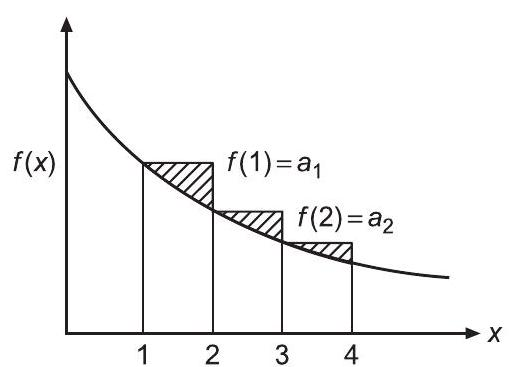
\includegraphics[max width=\textwidth, center]{2024_10_13_e0685a8ee0113ded3493g-06}\\
(a)\\
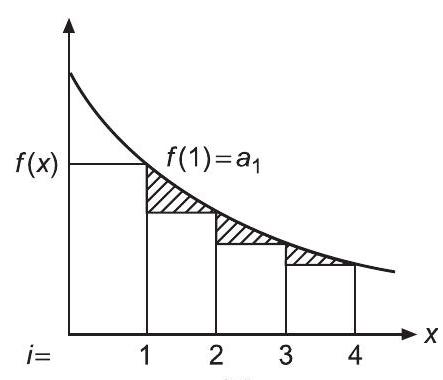
\includegraphics[max width=\textwidth, center]{2024_10_13_e0685a8ee0113ded3493g-06(1)}\\
(b)

FIGURE 1.1 (a) Comparison of integral and sum-blocks leading. (b) Comparison of integral and sum-blocks lagging.\\
and


\begin{equation*}
\int_{N+1}^{\infty} f(x) d x \leq \sum_{n=N+1}^{\infty} a_{n} \leq \int_{N+1}^{\infty} f(x) d x+a_{N+1} \tag{1.9}
\end{equation*}


To free the integral test from the quite restrictive requirement that the interpolating function $f(x)$ be positive and monotonic, we shall show that for any function $f(x)$ with a continuous derivative, the infinite series is exactly represented as a sum of two integrals:


\begin{equation*}
\sum_{n=N 1+1}^{N_{2}} f(n)=\int_{N_{1}}^{N_{2}} f(x) d x+\int_{N_{1}}^{N_{2}}(x-[x]) f^{\prime}(x) d x \tag{1.10}
\end{equation*}


Here $[x]$ is the integral part of $x$, i.e., the largest integer $\leq x$, so $x-[x]$ varies sawtoothlike between 0 and 1. Equation (1.10) is useful because if both integrals in Eq. (1.10) converge, the infinite series also converges, while if one integral converges and the other does not, the infinite series diverges. If both integrals diverge, the test fails unless it can be shown whether the divergences of the integrals cancel against each other.

We need now to establish Eq. (1.10). We manipulate the contributions to the second integral as follows:

\begin{enumerate}
  \item Using integration by parts, we observe that
\end{enumerate}

$$
\int_{N_{1}}^{N_{2}} x f^{\prime}(x) d x=N_{2} f\left(N_{2}\right)-N_{1} f\left(N_{1}\right)-\int_{N_{1}}^{N_{2}} f(x) d x
$$

\begin{enumerate}
  \setcounter{enumi}{1}
  \item We evaluate
\end{enumerate}

$$
\begin{aligned}
\int_{N_{1}}^{N_{2}}[x] f^{\prime}(x) d x & =\sum_{n=N_{1}}^{N_{2}-1} n \int_{n}^{n+1} f^{\prime}(x) d x=\sum_{n=N_{1}}^{N_{2}-1} n[f(n+1)-f(n)] \\
& =-\sum_{n=N_{1}+1}^{N_{2}} f(n)-N_{1} f\left(N_{1}\right)+N_{2} f\left(N_{2}\right)
\end{aligned}
$$

Subtracting the second of these equations from the first, we arrive at Eq. (1.10).

An alternative to Eq. (1.10) in which the second integral has its sawtooth shifted to be symmetrical about zero (and therefore perhaps smaller) can be derived by methods similar to those used above. The resulting formula is


\begin{align*}
\sum_{n=N 1+1}^{N_{2}} f(n)= & \int_{N_{1}}^{N_{2}} f(x) d x+\int_{N_{1}}^{N_{2}}\left(x-[x]-\frac{1}{2}\right) f^{\prime}(x) d x  \tag{1.11}\\
& +\frac{1}{2}\left[f\left(N_{2}\right)-f\left(N_{1}\right)\right]
\end{align*}


Because they do not use a monotonicity requirement, Eqs. (1.10) and (1.11) can be applied to alternating series, and even those with irregular sign sequences.

\section*{Example 1.1.5 Riemann Zeta Function}
The Riemann zeta function is defined by


\begin{equation*}
\zeta(p)=\sum_{n=1}^{\infty} n^{-p} \tag{1.12}
\end{equation*}


providing the series converges. We may take $f(x)=x^{-p}$, and then

$$
\begin{array}{rlr}
\int_{1}^{\infty} x^{-p} d x & =\left.\frac{x^{-p+1}}{-p+1}\right|_{x=1} ^{\infty}, & p \neq 1 \\
& =\left.\ln x\right|_{x=1} ^{\infty}, \quad p=1
\end{array}
$$

The integral and therefore the series are divergent for $p \leq 1$, and convergent for $p>1$. Hence Eq. (1.12) should carry the condition $p>1$. This, incidentally, is an independent proof that the harmonic series $(p=1)$ diverges logarithmically. The sum of the first million terms $\sum_{n=1}^{1,000,000} n^{-1}$ is only $14.392726 \cdots$.

While the harmonic series diverges, the combination


\begin{equation*}
\gamma=\lim _{n \rightarrow \infty}\left(\sum_{m=1}^{n} m^{-1}-\ln n\right) \tag{1.13}
\end{equation*}


converges, approaching a limit known as the Euler-Mascheroni constant.

\section*{Example 1.1.6 A Slowly DiverGing Series}
Consider now the series

$$
S=\sum_{n=2}^{\infty} \frac{1}{n \ln n}
$$

We form the integral

$$
\int_{2}^{\infty} \frac{1}{x \ln x} d x=\int_{x=2}^{\infty} \frac{d \ln x}{\ln x}=\left.\ln \ln x\right|_{x=2} ^{\infty}
$$

which diverges, indicating that $S$ is divergent. Note that the lower limit of the integral is in fact unimportant so long as it does not introduce any spurious singularities, as it is the large- $x$ behavior that determines the convergence. Because $n \ln n>n$, the divergence is slower than that of the harmonic series. But because $\ln n$ increases more slowly than $n^{\varepsilon}$, where $\varepsilon$ can have an arbitrarily small positive value, we have divergence even though the series $\sum_{n} n^{-(1+\varepsilon)}$ converges.

\section*{More Sensitive Tests}
Several tests more sensitive than those already examined are consequences of a theorem by Kummer. Kummer's theorem, which deals with two series of finite positive terms, $u_{n}$ and $a_{n}$, states:

\begin{enumerate}
  \item The series $\sum_{n} u_{n}$ converges if
\end{enumerate}


\begin{equation*}
\lim _{n \rightarrow \infty}\left(a_{n} \frac{u_{n}}{u_{n+1}}-a_{n+1}\right) \geq C>0 \tag{1.14}
\end{equation*}


where $C$ is a constant. This statement is equivalent to a simple comparison test if the series $\sum_{n} a_{n}^{-1}$ converges, and imparts new information only if that sum diverges. The more weakly $\sum_{n} a_{n}^{-1}$ diverges, the more powerful the Kummer test will be.\\
2. If $\sum_{n} a_{n}^{-1}$ diverges and


\begin{equation*}
\lim _{n \rightarrow \infty}\left(a_{n} \frac{u_{n}}{u_{n+1}}-a_{n+1}\right) \leq 0 \tag{1.15}
\end{equation*}


then $\sum_{n} u_{n}$ diverges.\\
The proof of this powerful test is remarkably simple. Part 2 follows immediately from the comparison test. To prove Part 1, write cases of Eq. (1.14) for $n=N+1$ through any larger $n$, in the following form:

$$
\begin{aligned}
u_{N+1} & \leq\left(a_{N} u_{N}-a_{N+1} u_{N+1}\right) / C \\
u_{N+2} & \leq\left(a_{N+1} u_{N+1}-a_{N+2} u_{N+2}\right) / C \\
\ldots & \leq \ldots \ldots \ldots \ldots \ldots \ldots \ldots \ldots \\
u_{n} & \leq\left(a_{n-1} u_{n-1}-a_{n} u_{n}\right) / C
\end{aligned}
$$

Adding, we get


\begin{align*}
\sum_{i=N+1}^{n} u_{i} & \leq \frac{a_{N} u_{N}}{C}-\frac{a_{n} u_{n}}{C}  \tag{1.16}\\
& <\frac{a_{N} u_{N}}{C} \tag{1.17}
\end{align*}


This shows that the tail of the series $\sum_{n} u_{n}$ is bounded, and that series is therefore proved convergent when Eq. (1.14) is satisfied for all sufficiently large $n$.

Gauss' test is an application of Kummer's theorem to series $u_{n}>0$ when the ratios of successive $u_{n}$ approach unity and the tests previously discussed yield indeterminate results. If for large $n$


\begin{equation*}
\frac{u_{n}}{u_{n+1}}=1+\frac{h}{n}+\frac{B(n)}{n^{2}} \tag{1.18}
\end{equation*}


where $B(n)$ is bounded for $n$ sufficiently large, then the Gauss test states that $\sum_{n} u_{n}$ converges for $h>1$ and diverges for $h \leq 1$ : There is no indeterminate case here.

The Gauss test is extremely sensitive, and will work for all troublesome series the physicist is likely to encounter. To confirm it using Kummer's theorem, we take $a_{n}=n \ln n$. The series $\sum_{n} a_{n}^{-1}$ is weakly divergent, as already established in Example 1.1.6.

Taking the limit on the left side of Eq. (1.14), we have


\begin{align*}
& \lim _{n \rightarrow \infty}\left[n \ln n\left(1+\frac{h}{n}+\frac{B(n)}{n^{2}}\right)-(n+1) \ln (n+1)\right] \\
& \quad=\lim _{n \rightarrow \infty}\left[(n+1) \ln n+(h-1) \ln n+\frac{B(n) \ln n}{n}-(n+1) \ln (n+1)\right] \\
& \quad=\lim _{n \rightarrow \infty}\left[-(n+1) \ln \left(\frac{n+1}{n}\right)+(h-1) \ln n\right] \tag{1.19}
\end{align*}


For $h<1$, both terms of Eq. (1.19) are negative, thereby signaling a divergent case of Kummer's theorem; for $h>1$, the second term of Eq. (1.19) dominates the first and is positive, indicating convergence. At $h=1$, the second term vanishes, and the first is inherently negative, thereby indicating divergence.

\section*{Example 1.1.7 LeGENDRE SERIES}
The series solution for the Legendre equation (encountered in Chapter 7) has successive terms whose ratio under certain conditions is

$$
\frac{a_{2 j+2}}{a_{2 j}}=\frac{2 j(2 j+1)-\lambda}{(2 j+1)(2 j+2)}
$$

To place this in the form now being used, we define $u_{j}=a_{2 j}$ and write

$$
\frac{u_{j}}{u_{j+1}}=\frac{(2 j+1)(2 j+2)}{2 j(2 j+1)-\lambda}
$$

In the limit of large $j$, the constant $\lambda$ becomes negligible (in the language of the Gauss test, it contributes to an extent $B(j) / j^{2}$, where $B(j)$ is bounded). We therefore have


\begin{equation*}
\frac{u_{j}}{u_{j+1}} \rightarrow \frac{2 j+2}{2 j}+\frac{B(j)}{j^{2}}=1+\frac{1}{j}+\frac{B(j)}{j^{2}} \tag{1.20}
\end{equation*}


The Gauss test tells us that this series is divergent.

\section*{Exercises}
1.1.1 (a) Prove that if $\lim _{n \rightarrow \infty} n^{p} u_{n}=A<\infty, p>1$, the series $\sum_{n=1}^{\infty} u_{n}$ converges.\\
(b) Prove that if $\lim _{n \rightarrow \infty} n u_{n}=A>0$, the series diverges. (The test fails for $A=0$.) These two tests, known as limit tests, are often convenient for establishing the convergence of a series. They may be treated as comparison tests, comparing with

$$
\sum_{n} n^{-q}, \quad 1 \leq q<p
$$

1.1.2 If $\lim _{n \rightarrow \infty} \frac{b_{n}}{a_{n}}=K$, a constant with $0<K<\infty$, show that $\Sigma_{n} b_{n}$ converges or diverges with $\Sigma a_{n}$.\\
Hint. If $\Sigma a_{n}$ converges, rescale $b_{n}$ to $b_{n}^{\prime}=\frac{b_{n}}{2 K}$. If $\Sigma_{n} a_{n}$ diverges, rescale to $b_{n}^{\prime \prime}=\frac{2 b_{n}}{K}$.\\
1.1.3 (a) Show that the series $\sum_{n=2}^{\infty} \frac{1}{n(\ln n)^{2}}$ converges.\\
(b) By direct addition $\sum_{n=2}^{100,000}\left[n(\ln n)^{2}\right]^{-1}=2.02288$. Use Eq. (1.9) to make a five-significant-figure estimate of the sum of this series.\\
1.1.4 Gauss' test is often given in the form of a test of the ratio

$$
\frac{u_{n}}{u_{n+1}}=\frac{n^{2}+a_{1} n+a_{0}}{n^{2}+b_{1} n+b_{0}}
$$

For what values of the parameters $a_{1}$ and $b_{1}$ is there convergence? divergence?

$$
\begin{aligned}
& \text { ANS. Convergent for } a_{1}-b_{1}>1 \text {, } \\
& \text { divergent for } a_{1}-b_{1} \leq 1 \text {. }
\end{aligned}
$$

\subsection*{1.1.5 Test for convergence}
(a) $\sum_{n=2}^{\infty}(\ln n)^{-1}$\\
(d) $\sum_{n=1}^{\infty}[n(n+1)]^{-1 / 2}$\\
(b) $\sum_{n=1}^{\infty} \frac{n!}{10^{n}}$\\
(e) $\sum_{n=0}^{\infty} \frac{1}{2 n+1}$\\
(c) $\sum_{n=1}^{\infty} \frac{1}{2 n(2 n+1)}$\\
1.1.6 Test for convergence\\
(a) $\sum_{n=1}^{\infty} \frac{1}{n(n+1)}$\\
(d) $\sum_{n=1}^{\infty} \ln \left(1+\frac{1}{n}\right)$\\
(b) $\sum_{n=2}^{\infty} \frac{1}{n \ln n}$\\
(e) $\sum_{n=1}^{\infty} \frac{1}{n \cdot n^{1 / n}}$\\
(c) $\sum_{n=1}^{\infty} \frac{1}{n 2^{n}}$\\
1.1.7 For what values of $p$ and $q$ will $\sum_{n=2}^{\infty} \frac{1}{n^{p}(\ln n)^{q}}$ converge?

$$
\text { ANS. } \quad \text { Convergent for }\left\{\begin{array} { l l } 
{ p > 1 , } & { \text { all } q , } \\
{ p = 1 , } & { q > 1 , }
\end{array} \quad \text { divergent for } \left\{\begin{array}{ll}
p<1, & \text { all } q \\
p=1, & q \leq 1
\end{array}\right.\right.
$$

1.1.8 Given $\sum_{n=1}^{1,000} n^{-1}=7.485470 \ldots$ set upper and lower bounds on the Euler-Mascheroni constant.

$$
\text { ANS. } \quad 0.5767<\gamma<0.5778
$$

1.1.9 (From Olbers' paradox.) Assume a static universe in which the stars are uniformly distributed. Divide all space into shells of constant thickness; the stars in any one shell by themselves subtend a solid angle of $\omega_{0}$. Allowing for the blocking out of distant stars by nearer stars, show that the total net solid angle subtended by all stars, shells extending to infinity, is exactly $4 \pi$. [Therefore the night sky should be ablaze with light. For more details, see E. Harrison, Darkness at Night: A Riddle of the Universe. Cambridge, MA: Harvard University Press (1987).]\\
1.1.10 Test for convergence

$$
\sum_{n=1}^{\infty}\left[\frac{1 \cdot 3 \cdot 5 \cdots(2 n-1)}{2 \cdot 4 \cdot 6 \cdots(2 n)}\right]^{2}=\frac{1}{4}+\frac{9}{64}+\frac{25}{256}+\cdots
$$

\section*{Alternating Series}
In previous subsections we limited ourselves to series of positive terms. Now, in contrast, we consider infinite series in which the signs alternate. The partial cancellation due to alternating signs makes convergence more rapid and much easier to identify. We shall prove the Leibniz criterion, a general condition for the convergence of an alternating series. For series with more irregular sign changes, the integral test of Eq. (1.10) is often helpful.

The Leibniz criterion applies to series of the form $\sum_{n=1}^{\infty}(-1)^{n+1} a_{n}$ with $a_{n}>0$, and states that if $a_{n}$ is monotonically decreasing (for sufficiently large $n$ ) and $\lim _{n \rightarrow \infty} a_{n}=0$, then the series converges. To prove this theorem, note that the remainder $R_{2 n}$ of the series beyond $s_{2 n}$, the partial sum after $2 n$ terms, can be written in two alternate ways:

$$
\begin{aligned}
R_{2 n} & =\left(a_{2 n+1}-a_{2 n+2}\right)+\left(a_{2 n+3}-a_{2 n+4}\right)+\cdots \\
& =a_{2 n+1}-\left(a_{2 n+2}-a_{2 n+3}\right)-\left(a_{2 n+4}-a_{2 n+5}\right)-\cdots
\end{aligned}
$$

Since the $a_{n}$ are decreasing, the first of these equations implies $R_{2 n}>0$, while the second implies $R_{2 n}<a_{2 n+1}$, so

$$
0<R_{2 n}<a_{2 n+1}
$$

Thus, $R_{2 n}$ is positive but bounded, and the bound can be made arbitrarily small by taking larger values of $n$. This demonstration also shows that the error from truncating an alternating series after $a_{2 n}$ results in an error that is negative (the omitted terms were shown to combine to a positive result) and bounded in magnitude by $a_{2 n+1}$. An argument similar to that made above for the remainder after an odd number of terms, $R_{2 n+1}$, would show that the error from truncation after $a_{2 n+1}$ is positive and bounded by $a_{2 n+2}$. Thus, it is generally true that the error in truncating an alternating series with monotonically decreasing terms is of the same sign as the last term kept and smaller than the first term dropped.

The Leibniz criterion depends for its applicability on the presence of strict sign alternation. Less regular sign changes present more challenging problems for convergence determination.

\section*{Example 1.1.8 Series with IrRegular Sign Changes}
For $0<x<2 \pi$, the series


\begin{equation*}
S=\sum_{n=1}^{\infty} \frac{\cos (n x)}{n}=-\ln \left(2 \sin \frac{x}{2}\right) \tag{1.21}
\end{equation*}


converges, having coefficients that change sign often, but not so that the Leibniz criterion applies easily. To verify the convergence, we apply the integral test of Eq. (1.10), inserting the explicit form for the derivative of $\cos (n x) / n$ (with respect to $n$ ) in the second integral:


\begin{equation*}
S=\int_{1}^{\infty} \frac{\cos (n x)}{n} d n+\int_{1}^{\infty}(n-[n])\left[-\frac{x}{n} \sin (n x)-\frac{\cos (n x)}{n^{2}}\right] d n \tag{1.22}
\end{equation*}


Using integration by parts, the first integral in Eq. (1.22) is rearranged to

$$
\int_{1}^{\infty} \frac{\cos (n x)}{n} d n=\left[\frac{\sin (n x)}{n x}\right]_{1}^{\infty}+\frac{1}{x} \int_{1}^{\infty} \frac{\sin (n x)}{n^{2}} d n
$$

and this integral converges because

$$
\left|\int_{1}^{\infty} \frac{\sin (n x)}{n^{2}} d n\right|<\int_{1}^{\infty} \frac{d n}{n^{2}}=1
$$

Looking now at the second integral in Eq. (1.22), we note that its term $\cos (n x) / n^{2}$ also leads to a convergent integral, so we need only to examine the convergence of

$$
\int_{1}^{\infty}(n-[n]) \frac{\sin (n x)}{n} d n
$$

Next, setting $(n-[n]) \sin (n x)=g^{\prime}(n)$, which is equivalent to defining $g(N)=\int_{1}^{N}(n-$ $[n]) \sin (n x) d n$, we write

$$
\int_{1}^{\infty}(n-[n]) \frac{\sin (n x)}{n} d n=\int_{1}^{\infty} \frac{g^{\prime}(n)}{n} d n=\left[\frac{g(n)}{n}\right]_{n=1}^{\infty}+\int_{1}^{\infty} \frac{g(n)}{n^{2}} d n
$$

where the last equality was obtained using once again an integration by parts. We do not have an explicit expression for $g(n)$, but we do know that it is bounded because $\sin x$ oscillates with a period incommensurate with that of the sawtooth periodicity of $(n-[n])$. This boundedness enables us to determine that the second integral in Eq. (1.22) converges, thus establishing the convergence of $S$.

\section*{Absolute and Conditional Convergence}
An infinite series is absolutely convergent if the absolute values of its terms form a convergent series. If it converges, but not absolutely, it is termed conditionally convergent. An example of a conditionally convergent series is the alternating harmonic series,


\begin{equation*}
\sum_{n=1}^{\infty}(-1)^{n-1} n^{-1}=1-\frac{1}{2}+\frac{1}{3}-\frac{1}{4}+\cdots+\frac{(-1)^{n-1}}{n}+\cdots \tag{1.23}
\end{equation*}


This series is convergent, based on the Leibniz criterion. It is clearly not absolutely convergent; if all terms are taken with + signs, we have the harmonic series, which we already know to be divergent. The tests described earlier in this section for series of positive terms are, then, tests for absolute convergence.

\section*{Exercises}
1.1.11 Determine whether each of these series is convergent, and if so, whether it is absolutely convergent:\\
(a) $\frac{\ln 2}{2}-\frac{\ln 3}{3}+\frac{\ln 4}{4}-\frac{\ln 5}{5}+\frac{\ln 6}{6}-\cdots$,\\
(b) $\frac{1}{1}+\frac{1}{2}-\frac{1}{3}-\frac{1}{4}+\frac{1}{5}+\frac{1}{6}-\frac{1}{7}-\frac{1}{8}+\cdots$,\\
(c) $1-\frac{1}{2}-\frac{1}{3}+\frac{1}{4}+\frac{1}{5}+\frac{1}{6}-\frac{1}{7}-\frac{1}{8}-\frac{1}{9}-\frac{1}{10}+\frac{1}{11} \cdots+\frac{1}{15}-\frac{1}{16} \cdots-\frac{1}{21}+\cdots$.\\
1.1.12 Catalan's constant $\beta(2)$ is defined by

$$
\beta(2)=\sum_{k=0}^{\infty}(-1)^{k}(2 k+1)^{-2}=\frac{1}{1^{2}}-\frac{1}{3^{2}}+\frac{1}{5^{2}} \cdots
$$

Calculate $\beta(2)$ to six-digit accuracy.

Hint. The rate of convergence is enhanced by pairing the terms,

$$
(4 k-1)^{-2}-(4 k+1)^{-2}=\frac{16 k}{\left(16 k^{2}-1\right)^{2}}
$$

If you have carried enough digits in your summation, $\sum_{1 \leq k \leq N} 16 k /\left(16 k^{2}-1\right)^{2}$, additional significant figures may be obtained by setting upper and lower bounds on the tail of the series, $\sum_{k=N+1}^{\infty}$. These bounds may be set by comparison with integrals, as in the Maclaurin integral test.

$$
\text { ANS. } \quad \beta(2)=0.915965594177 \cdots
$$

\section*{Operations on Series}
We now investigate the operations that may be performed on infinite series. In this connection the establishment of absolute convergence is important, because it can be proved that the terms of an absolutely convergent series may be reordered according to the familiar rules of algebra or arithmetic:

\begin{itemize}
  \item If an infinite series is absolutely convergent, the series sum is independent of the order in which the terms are added.
  \item An absolutely convergent series may be added termwise to, or subtracted termwise from, or multiplied termwise with another absolutely convergent series, and the resulting series will also be absolutely convergent.
  \item The series (as a whole) may be multiplied with another absolutely convergent series. The limit of the product will be the product of the individual series limits. The product series, a double series, will also converge absolutely.
\end{itemize}

No such guarantees can be given for conditionally convergent series, though some of the above properties remain true if only one of the series to be combined is conditionally convergent.

\section*{Example 1.1.9 Rearrangement of Alternating Harmonic Series}
Writing the alternating harmonic series as


\begin{equation*}
1-\frac{1}{2}+\frac{1}{3}-\frac{1}{4}+\cdots=1-\left(\frac{1}{2}-\frac{1}{3}\right)-\left(\frac{1}{4}-\frac{1}{5}\right)-\cdots \tag{1.24}
\end{equation*}


it is clear that $\sum_{n=1}^{\infty}(-1)^{n-1} n^{-1}<1$. However, if we rearrange the order of the terms, we can make this series converge to $\frac{3}{2}$. We regroup the terms of Eq. (1.24), as


\begin{align*}
& \left(1+\frac{1}{3}+\frac{1}{5}\right)-\left(\frac{1}{2}\right)+\left(\frac{1}{7}+\frac{1}{9}+\frac{1}{11}+\frac{1}{13}+\frac{1}{15}\right) \\
& -\left(\frac{1}{4}\right)+\left(\frac{1}{17}+\cdots+\frac{1}{25}\right)-\left(\frac{1}{6}\right)+\left(\frac{1}{27}+\cdots+\frac{1}{35}\right)-\left(\frac{1}{8}\right)+\cdots \tag{1.25}
\end{align*}


\begin{center}
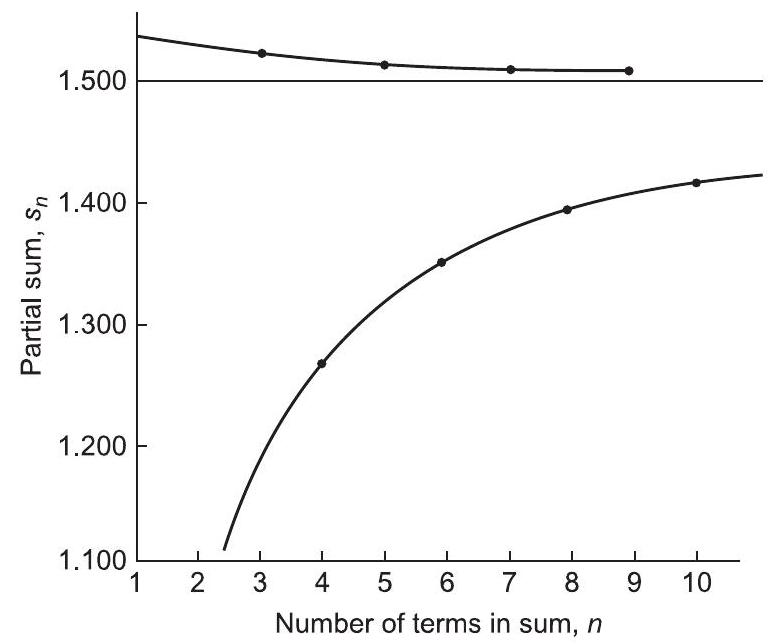
\includegraphics[max width=\textwidth]{2024_10_13_e0685a8ee0113ded3493g-15}
\end{center}

Figure 1.2 Alternating harmonic series. Terms are rearranged to give convergence to 1.5 .

Treating the terms grouped in parentheses as single terms for convenience, we obtain the partial sums

$$
\begin{array}{ll}
s_{1}=1.5333 & s_{2}=1.0333 \\
s_{3}=1.5218 & s_{4}=1.2718 \\
s_{5}=1.5143 & s_{6}=1.3476 \\
s_{7}=1.5103 & s_{8}=1.3853 \\
s_{9}=1.5078 & s_{10}=1.4078
\end{array}
$$

From this tabulation of $s_{n}$ and the plot of $s_{n}$ versus $n$ in Fig. 1.2, the convergence to $\frac{3}{2}$ is fairly clear. Our rearrangement was to take positive terms until the partial sum was equal to or greater than $\frac{3}{2}$ and then to add negative terms until the partial sum just fell below $\frac{3}{2}$ and so on. As the series extends to infinity, all original terms will eventually appear, but the partial sums of this rearranged alternating harmonic series converge to $\frac{3}{2}$.

As the example shows, by a suitable rearrangement of terms, a conditionally convergent series may be made to converge to any desired value or even to diverge. This statement is sometimes called Riemann's theorem.\\
Another example shows the danger of multiplying conditionally convergent series.

\section*{Example 1.1.10 Square of a Conditionally Convergent Series May Diverge}
The series $\sum_{n=1}^{\infty} \frac{(-1)^{n-1}}{\sqrt{n}}$ converges by the Leibniz criterion. Its square,

$$
\left[\sum_{n=1}^{\infty} \frac{(-1)^{n-1}}{\sqrt{n}}\right]^{2}=\sum_{n}(-1)^{n}\left[\frac{1}{\sqrt{1}} \frac{1}{\sqrt{n-1}}+\frac{1}{\sqrt{2}} \frac{1}{\sqrt{n-2}}+\cdots+\frac{1}{\sqrt{n-1}} \frac{1}{\sqrt{1}}\right]
$$

has a general term, in [ $\ldots$ ], consisting of $n-1$ additive terms, each of which is bigger than $\frac{1}{\sqrt{n-1} \sqrt{n-1}}$, so the entire [...] term is greater than $\frac{n-1}{n-1}$ and does not go to zero. Hence the general term of this product series does not approach zero in the limit of large $n$ and the series diverges.

These examples show that conditionally convergent series must be treated with caution.

\section*{Improvement of Convergence}
This section so far has been concerned with establishing convergence as an abstract mathematical property. In practice, the rate of convergence may be of considerable importance. A method for improving convergence, due to Kummer, is to form a linear combination of our slowly converging series and one or more series whose sum is known. For the known series the following collection is particularly useful:


\begin{align*}
\alpha_{1} & =\sum_{n=1}^{\infty} \frac{1}{n(n+1)}=1 \\
\alpha_{2} & =\sum_{n=1}^{\infty} \frac{1}{n(n+1)(n+2)}=\frac{1}{4} \\
\alpha_{3} & =\sum_{n=1}^{\infty} \frac{1}{n(n+1)(n+2)(n+3)}=\frac{1}{18} \\
& \ldots \ldots \ldots \ldots \ldots \ldots \ldots \ldots  \tag{1.26}\\
\alpha_{p} & =\sum_{n=1}^{\infty} \frac{1}{n(n+1) \cdots(n+p)}=\frac{1}{p p!}
\end{align*}


These sums can be evaluated via partial fraction expansions, and are the subject of Exercise 1.5.3.

The series we wish to sum and one or more known series (multiplied by coefficients) are combined term by term. The coefficients in the linear combination are chosen to cancel the most slowly converging terms.

\section*{Example 1.1.11 Riemann Zeta Function $\zeta(3)$}
From the definition in Eq. (1.12), we identify $\zeta$ (3) as $\sum_{n=1}^{\infty} n^{-3}$. Noting that $\alpha_{2}$ of Eq. (1.26) has a large- $n$ dependence $\sim n^{-3}$, we consider the linear combination


\begin{equation*}
\sum_{n=1}^{\infty} n^{-3}+a \alpha_{2}=\zeta(3)+\frac{a}{4} \tag{1.27}
\end{equation*}


We did not use $\alpha_{1}$ because it converges more slowly than $\zeta(3)$. Combining the two series on the left-hand side termwise, we obtain

$$
\sum_{n=1}^{\infty}\left[\frac{1}{n^{3}}+\frac{a}{n(n+1)(n+2)}\right]=\sum_{n=1}^{\infty} \frac{n^{2}(1+a)+3 n+2}{n^{3}(n+1)(n+2)}
$$

Table 1.1 Riemann Zeta Function

\begin{center}
\begin{tabular}{cc}
\hline
$s$ & $\zeta(s)$ \\
\hline
2 & 1.6449340668 \\
3 & 1.2020569032 \\
4 & 1.0823232337 \\
5 & 1.0369277551 \\
6 & 1.0173430620 \\
7 & 1.0083492774 \\
8 & 1.0040773562 \\
9 & 1.0020083928 \\
10 & 1.0009945751 \\
\hline
\end{tabular}
\end{center}

If we choose $a=-1$, we remove the leading term from the numerator; then, setting this equal to the right-hand side of Eq. (1.27) and solving for $\zeta(3)$,


\begin{equation*}
\zeta(3)=\frac{1}{4}+\sum_{n=1}^{\infty} \frac{3 n+2}{n^{3}(n+1)(n+2)} \tag{1.28}
\end{equation*}


The resulting series may not be beautiful but it does converge as $n^{-4}$, faster than $n^{-3}$. A more convenient form with even faster convergence is introduced in Exercise 1.1.16. There, the symmetry leads to convergence as $n^{-5}$.

Sometimes it is helpful to use the Riemann zeta function in a way similar to that illustrated for the $\alpha_{p}$ in the foregoing example. That approach is practical because the zeta function has been tabulated (see Table 1.1).

\section*{Example 1.1.12 CONVERGENCE IMPROVEMENT}
The problem is to evaluate the series $\sum_{n=1}^{\infty} 1 /\left(1+n^{2}\right)$. Expanding $\left(1+n^{2}\right)^{-1}=n^{-2}(1+$ $\left.n^{-2}\right)^{-1}$ by direct division, we have

$$
\begin{aligned}
\left(1+n^{2}\right)^{-1} & =n^{-2}\left(1-n^{-2}+n^{-4}-\frac{n^{-6}}{1+n^{-2}}\right) \\
& =\frac{1}{n^{2}}-\frac{1}{n^{4}}+\frac{1}{n^{6}}-\frac{1}{n^{8}+n^{6}}
\end{aligned}
$$

Therefore

$$
\sum_{n=1}^{\infty} \frac{1}{1+n^{2}}=\zeta(2)-\zeta(4)+\zeta(6)-\sum_{n=1}^{\infty} \frac{1}{n^{8}+n^{6}}
$$

The remainder series converges as $n^{-8}$. Clearly, the process can be continued as desired. You make a choice between how much algebra you will do and how much arithmetic the computer will do.

\section*{Rearrangement of Double Series}
An absolutely convergent double series (one whose terms are identified by two summation indices) presents interesting rearrangement opportunities. Consider


\begin{equation*}
S=\sum_{m=0}^{\infty} \sum_{n=0}^{\infty} a_{n, m} \tag{1.29}
\end{equation*}


In addition to the obvious possibility of reversing the order of summation (i.e., doing the $m$ sum first), we can make rearrangements that are more innovative. One reason for doing this is that we may be able to reduce the double sum to a single summation, or even evaluate the entire double sum in closed form.

As an example, suppose we make the following index substitutions in our double series: $m=q, n=p-q$. Then we will cover all $n \geq 0, m \geq 0$ by assigning $p$ the range $(0, \infty)$, and $q$ the range $(0, p)$, so our double series can be written


\begin{equation*}
S=\sum_{p=0}^{\infty} \sum_{q=0}^{p} a_{p-q, q} \tag{1.30}
\end{equation*}


In the $n m$ plane our region of summation is the entire quadrant $m \geq 0, n \geq 0$; in the $p q$ plane our summation is over the triangular region sketched in Fig. 1.3. This same $p q$ region can be covered when the summations are carried out in the reverse order, but with limits

$$
S=\sum_{q=0}^{\infty} \sum_{p=q}^{\infty} a_{p-q, q}
$$

The important thing to note here is that these schemes all have in common that, by allowing the indices to run over their designated ranges, every $a_{n, m}$ is eventually encountered, and is encountered exactly once.\\
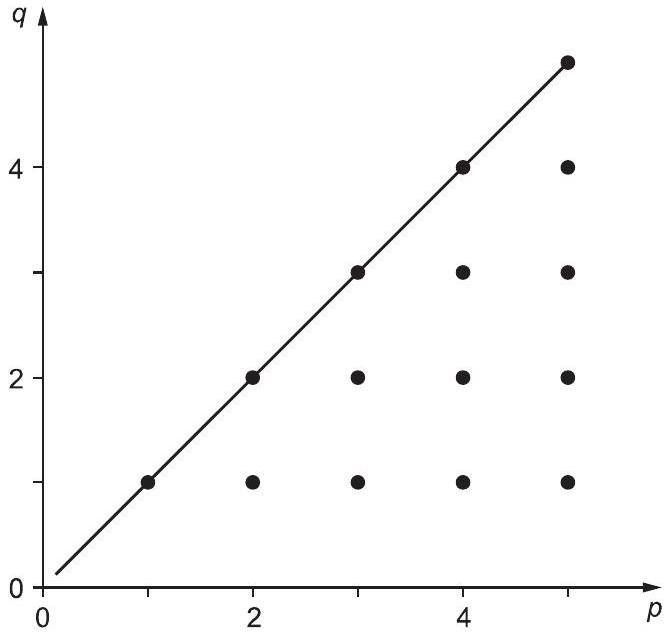
\includegraphics[max width=\textwidth, center]{2024_10_13_e0685a8ee0113ded3493g-18}

Figure 1.3 The $p q$ index space.

Another possible index substitution is to set $n=s, m=r-2 s$. If we sum over $s$ first, its range must be $(0,[r / 2])$, where $[r / 2]$ is the integer part of $r / 2$, i.e., $[r / 2]=r / 2$ for $r$ even and $(r-1) / 2$ for $r$ odd. The range of $r$ is $(0, \infty)$. This situation corresponds to


\begin{equation*}
S=\sum_{r=0}^{\infty} \sum_{s=0}^{[r / 2]} a_{s, r-2 s} \tag{1.31}
\end{equation*}


The sketches in Figs. 1.4 to 1.6 show the order in which the $a_{n, m}$ are summed when using the forms given in Eqs. (1.29), (1.30), and (1.31), respectively.\\
If the double series introduced originally as Eq. (1.29) is absolutely convergent, then all these rearrangements will give the same ultimate result.\\
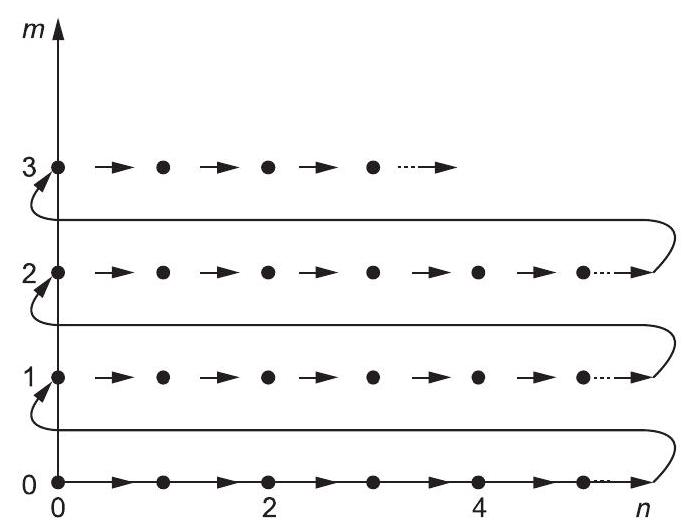
\includegraphics[max width=\textwidth, center]{2024_10_13_e0685a8ee0113ded3493g-19}

Figure 1.4 Order in which terms are summed with $m, n$ index set, Eq. (1.29).\\
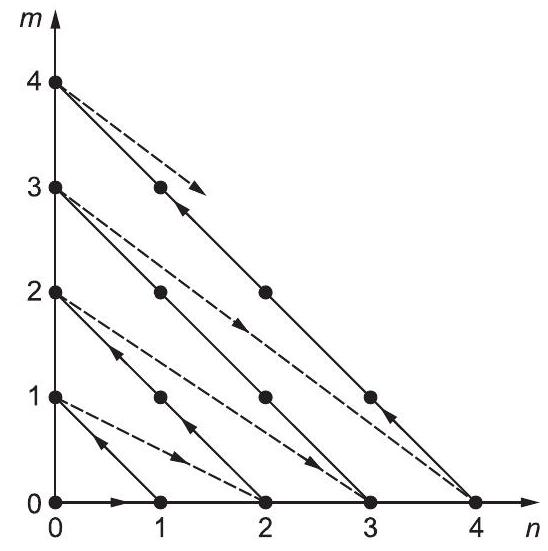
\includegraphics[max width=\textwidth, center]{2024_10_13_e0685a8ee0113ded3493g-19(1)}

Figure 1.5 Order in which terms are summed with $p, q$ index set, Eq. (1.30).\\
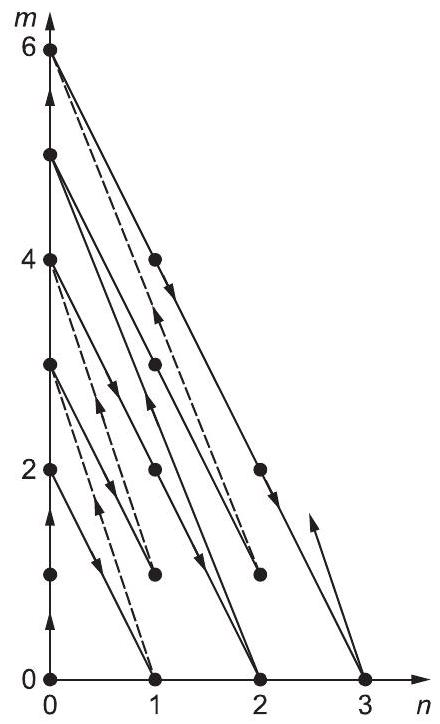
\includegraphics[max width=\textwidth, center]{2024_10_13_e0685a8ee0113ded3493g-20}

Figure 1.6 Order in which terms are summed with $r, s$ index set, Eq. (1.31).

\section*{Exercises}
1.1.13 Show how to combine $\zeta(2)=\sum_{n=1}^{\infty} n^{-2}$ with $\alpha_{1}$ and $\alpha_{2}$ to obtain a series converging as $n^{-4}$.\\
Note. $\zeta$ (2) has the known value $\pi^{2} / 6$. See Eq. (12.66).\\
1.1.14 Give a method of computing

$$
\lambda(3)=\sum_{n=0}^{\infty} \frac{1}{(2 n+1)^{3}}
$$

that converges at least as fast as $n^{-8}$ and obtain a result good to six decimal places.\\
ANS. $\quad \lambda(3)=1.051800$.\\
1.1.15 Show that (a) $\sum_{n=2}^{\infty}[\zeta(n)-1]=1, \quad$ (b) $\sum_{n=2}^{\infty}(-1)^{n}[\zeta(n)-1]=\frac{1}{2}$, where $\zeta(n)$ is the Riemann zeta function.\\
1.1.16 The convergence improvement of 1.1.11 may be carried out more expediently (in this special case) by putting $\alpha_{2}$, from Eq. (1.26), into a more symmetric form: Replacing $n$ by $n-1$, we have

$$
\alpha_{2}^{\prime}=\sum_{n=2}^{\infty} \frac{1}{(n-1) n(n+1)}=\frac{1}{4}
$$

(a) Combine $\zeta$ (3) and $\alpha_{2}^{\prime}$ to obtain convergence as $n^{-5}$.\\
(b) Let $\alpha_{4}^{\prime}$ be $\alpha_{4}$ with $n \rightarrow n-2$. Combine $\zeta(3), \alpha_{2}^{\prime}$, and $\alpha_{4}^{\prime}$ to obtain convergence as $n^{-7}$.\\
(c) If $\zeta(3)$ is to be calculated to six-decimal place accuracy (error $5 \times 10^{-7}$ ), how many terms are required for $\zeta(3)$ alone? combined as in part (a)? combined as in part (b)?

Note. The error may be estimated using the corresponding integral.\\
ANS.

$$
\text { (a) } \quad \zeta(3)=\frac{5}{4}-\sum_{n=2}^{\infty} \frac{1}{n^{3}\left(n^{2}-1\right)}
$$

\subsection*{1.2 SERIES OF FUNCTIONS}
We extend our concept of infinite series to include the possibility that each term $u_{n}$ may be a function of some variable, $u_{n}=u_{n}(x)$. The partial sums become functions of the variable $x$,


\begin{equation*}
s_{n}(x)=u_{1}(x)+u_{2}(x)+\cdots+u_{n}(x) \tag{1.32}
\end{equation*}


as does the series sum, defined as the limit of the partial sums:


\begin{equation*}
\sum_{n=1}^{\infty} u_{n}(x)=S(x)=\lim _{n \rightarrow \infty} s_{n}(x) \tag{1.33}
\end{equation*}


So far we have concerned ourselves with the behavior of the partial sums as a function of $n$. Now we consider how the foregoing quantities depend on $x$. The key concept here is that of uniform convergence.

\section*{Uniform Convergence}
If for any small $\varepsilon>0$ there exists a number $N$, independent of $\boldsymbol{x}$ in the interval $[a, b]$ (that is, $a \leq x \leq b$ ) such that


\begin{equation*}
\left|S(x)-s_{n}(x)\right|<\varepsilon, \quad \text { for all } n \geq N \tag{1.34}
\end{equation*}


then the series is said to be uniformly convergent in the interval $[a, b]$. This says that for our series to be uniformly convergent, it must be possible to find a finite $N$ so that the absolute value of the tail of the infinite series, $\left|\sum_{i=N+1}^{\infty} u_{i}(x)\right|$, will be less than an arbitrary small $\varepsilon$ for all $x$ in the given interval, including the endpoints.

\section*{Example 1.2.1 NONUNIFORM CONVERGENCE}
Consider on the interval $[0,1]$ the series

$$
S(x)=\sum_{n=0}^{\infty}(1-x) x^{n}
$$

For $0 \leq x<1$, the geometric series $\sum_{n} x^{n}$ is convergent, with value $1 /(1-x)$, so $S(x)=$ 1 for these $x$ values. But at $x=1$, every term of the series will be zero, and therefore $S(1)=0$. That is,


\begin{align*}
\sum_{n=0}^{\infty}(1-x) x^{n} & =1, \quad 0 \leq x<1 \\
& =0, \quad x=1 \tag{1.35}
\end{align*}


So $S(x)$ is convergent for the entire interval [0,1], and because each term is nonnegative, it is also absolutely convergent. If $x \neq 0$, this is a series for which the partial sum $s_{N}$ is $1-x^{N}$, as can be seen by comparison with Eq. (1.3). Since $S(x)=1$, the uniform convergence criterion is

$$
\left|1-\left(1-x^{N}\right)\right|=x^{N}<\varepsilon
$$

No matter what the values of $N$ and a sufficiently small $\varepsilon$ may be, there will be an $x$ value (close to 1 ) where this criterion is violated. The underlying problem is that $x=1$ is the convergence limit of the geometric series, and it is not possible to have a convergence rate that is bounded independently of $x$ in a range that includes $x=1$.

We note also from this example that absolute and uniform convergence are independent concepts. The series in this example has absolute, but not uniform convergence. We will shortly present examples of series that are uniformly, but only conditionally convergent. And there are series that have neither or both of these properties.

\section*{Weierstrass $M$ (Majorant) Test}
The most commonly encountered test for uniform convergence is the Weierstrass $M$ test. If we can construct a series of numbers $\sum_{i=1}^{\infty} M_{i}$, in which $M_{i} \geq\left|u_{i}(x)\right|$ for all $x$ in the interval $[a, b]$ and $\sum_{i=1}^{\infty} M_{i}$ is convergent, our series $u_{i}(x)$ will be uniformly convergent in $[a, b]$.

The proof of this Weierstrass $M$ test is direct and simple. Since $\sum_{i} M_{i}$ converges, some number $N$ exists such that for $n+1 \geq N$,

$$
\sum_{i=n+1}^{\infty} M_{i}<\varepsilon
$$

This follows from our definition of convergence. Then, with $\left|u_{i}(x)\right| \leq M_{i}$ for all $x$ in the interval $a \leq x \leq b$,

$$
\sum_{i=n+1}^{\infty} u_{i}(x)<\varepsilon
$$

Hence $S(x)=\sum_{n=1}^{\infty} u_{i}(x)$ satisfies


\begin{equation*}
\left|S(x)-s_{n}(x)\right|=\left|\sum_{i=n+1}^{\infty} u_{i}(x)\right|<\varepsilon \tag{1.36}
\end{equation*}


we see that $\sum_{n=1}^{\infty} u_{i}(x)$ is uniformly convergent in $[a, b]$. Since we have specified absolute values in the statement of the Weierstrass $M$ test, the series $\sum_{n=1}^{\infty} u_{i}(x)$ is also seen to be absolutely convergent. As we have already observed in Example 1.2.1, absolute and uniform convergence are different concepts, and one of the limitations of the Weierstrass $M$ test is that it can only establish uniform convergence for series that are also absolutely convergent.\\
To further underscore the difference between absolute and uniform convergence, we provide another example.

\section*{Example 1.2.2 Uniformly ConVergent Alternating SERIES}
Consider the series


\begin{equation*}
S(x)=\sum_{n=1}^{\infty} \frac{(-1)^{n}}{n+x^{2}}, \quad-\infty<x<\infty \tag{1.37}
\end{equation*}


Applying the Leibniz criterion, this series is easily proven convergent for the entire interval $-\infty<x<\infty$, but it is not absolutely convergent, as the absolute values of its terms approach for large $n$ those of the divergent harmonic series. The divergence of the absolute value series is obvious at $x=0$, where we then exactly have the harmonic series. Nevertheless, this series is uniformly convergent on $-\infty<x<\infty$, as its convergence is for all $x$ at least as fast as it is for $x=0$. More formally,

$$
\left|S(x)-s_{n}(x)\right|<\left|u_{n+1}(x)\right| \leq\left|u_{n+1}(0)\right|
$$

Since $u_{n+1}(0)$ is independent of $x$, uniform convergence is confirmed.

\section*{Abel's Test}
A somewhat more delicate test for uniform convergence has been given by Abel. If $u_{n}(x)$ can be written in the form $a_{n} f_{n}(x)$, and

\begin{enumerate}
  \item The $a_{n}$ form a convergent series, $\sum_{n} a_{n}=A$,
  \item For all $x$ in $[a, b]$ the functions $f_{n}(x)$ are monotonically decreasing in $n$, i.e., $f_{n+1}(x) \leq$ $f_{n}(x)$,
  \item For all $x$ in $[a, b]$ all the $f(n)$ are bounded in the range $0 \leq f_{n}(x) \leq M$, where $M$ is independent of $x$,\\
then $\sum_{n} u_{n}(x)$ converges uniformly in $[a, b]$.\\
This test is especially useful in analyzing the convergence of power series. Details of the proof of Abel's test and other tests for uniform convergence are given in the works by Knopp and by Whittaker and Watson (see Additional Readings listed at the end of this chapter).
\end{enumerate}

\section*{Properties of Uniformly Convergent Series}
Uniformly convergent series have three particularly useful properties. If a series $\sum_{n} u_{n}(x)$ is uniformly convergent in $[a, b]$ and the individual terms $u_{n}(x)$ are continuous,

\begin{enumerate}
  \item The series sum $S(x)=\sum_{n=1}^{\infty} u_{n}(x)$ is also continuous.
  \item The series may be integrated term by term. The sum of the integrals is equal to the integral of the sum:
\end{enumerate}


\begin{equation*}
\int_{a}^{b} S(x) d x=\sum_{n=1}^{\infty} \int_{a}^{b} u_{n}(x) d x \tag{1.38}
\end{equation*}


\begin{enumerate}
  \setcounter{enumi}{2}
  \item The derivative of the series sum $S(x)$ equals the sum of the individual-term derivatives:
\end{enumerate}


\begin{equation*}
\frac{d}{d x} S(x)=\sum_{n=1}^{\infty} \frac{d}{d x} u_{n}(x) \tag{1.39}
\end{equation*}


provided the following additional conditions are satisfied:

$$
\begin{aligned}
& \frac{d u_{n}(x)}{d x} \text { is continuous in }[a, b] \\
& \sum_{n=1}^{\infty} \frac{d u_{n}(x)}{d x} \text { is uniformly convergent in }[a, b]
\end{aligned}
$$

Term-by-term integration of a uniformly convergent series requires only continuity of the individual terms. This condition is almost always satisfied in physical applications. Term-by-term differentiation of a series is often not valid because more restrictive conditions must be satisfied.

\section*{Exercises}
1.2.1 Find the range of uniform convergence of the series\\
(a) $\eta(x)=\sum_{n=1}^{\infty} \frac{(-1)^{n-1}}{n^{x}}$,\\
(b) $\zeta(x)=\sum_{n=1}^{\infty} \frac{1}{n^{x}}$.

ANS. (a) $0<s \leq x<\infty$.\\
(b) $1<s \leq x<\infty$.\\
1.2.2 For what range of $x$ is the geometric series $\sum_{n=0}^{\infty} x^{n}$ uniformly convergent?

$$
\text { ANS. } \quad-1<-s \leq x \leq s<1
$$

1.2.3 For what range of positive values of $x$ is $\sum_{n=0}^{\infty} 1 /\left(1+x^{n}\right)$\\
(a) convergent?\\
(b) uniformly convergent?\\
1.2.4 If the series of the coefficients $\sum a_{n}$ and $\sum b_{n}$ are absolutely convergent, show that the Fourier series

$$
\sum\left(a_{n} \cos n x+b_{n} \sin n x\right)
$$

is uniformly convergent for $-\infty<x<\infty$.\\
1.2.5 The Legendre series $\sum_{j \text { even }} u_{j}(x)$ satisfies the recurrence relations

$$
u_{j+2}(x)=\frac{(j+1)(j+2)-l(l+1)}{(j+2)(j+3)} x^{2} u_{j}(x)
$$

in which the index $j$ is even and $l$ is some constant (but, in this problem, not a nonnegative odd integer). Find the range of values of $x$ for which this Legendre series is convergent. Test the endpoints.

$$
\text { ANS. } \quad-1<x<1
$$

1.2.6 A series solution of the Chebyshev equation leads to successive terms having the ratio

$$
\frac{u_{j+2}(x)}{u_{j}(x)}=\frac{(k+j)^{2}-n^{2}}{(k+j+1)(k+j+2)} x^{2}
$$

with $k=0$ and $k=1$. Test for convergence at $x= \pm 1$.\\
ANS. Convergent.\\
1.2.7 A series solution for the ultraspherical (Gegenbauer) function $C_{n}^{\alpha}(x)$ leads to the recurrence

$$
a_{j+2}=a_{j} \frac{(k+j)(k+j+2 \alpha)-n(n+2 \alpha)}{(k+j+1)(k+j+2)}
$$

Investigate the convergence of each of these series at $x= \pm 1$ as a function of the parameter $\alpha$.

ANS. Convergent for $\alpha<1$, divergent for $\alpha \geq 1$.

\section*{Taylor's Expansion}
Taylor's expansion is a powerful tool for the generation of power series representations of functions. The derivation presented here provides not only the possibility of an expansion into a finite number of terms plus a remainder that may or may not be easy to evaluate, but also the possibility of the expression of a function as an infinite series of powers.

We assume that our function $f(x)$ has a continuous $n$th derivative ${ }^{2}$ in the interval $a \leq$ $x \leq b$. We integrate this $n$th derivative $n$ times; the first three integrations yield

$$
\begin{aligned}
& \int_{a}^{x} f^{(n)}\left(x_{1}\right) d x_{1}=\left.f^{(n-1)}\left(x_{1}\right)\right|_{a} ^{x}=f^{(n-1)}(x)-f^{(n-1)}(a), \\
& \int_{a}^{x} d x_{2} \int_{a}^{x_{2}} f^{(n)}\left(x_{1}\right) d x_{1}=\int_{a}^{x} d x_{2}\left[f^{(n-1)}\left(x_{2}\right)-f^{(n-1)}(a)\right] \\
& =f^{(n-2)}(x)-f^{(n-2)}(a)-(x-a) f^{(n-1)}(a), \\
& \int_{a}^{x} d x_{3} \int_{a}^{x_{3}} d x_{2} \int_{a}^{x_{2}} f^{(n)}\left(x_{1}\right) d x_{1}=f^{(n-3)}(x)-f^{(n-3)}(a) \\
& -(x-a) f^{(n-2)}(a)-\frac{(x-a)^{2}}{2!} f^{(n-1)}(a) .
\end{aligned}
$$

Finally, after integrating for the $n$th time,

$$
\begin{aligned}
\int_{a}^{x} d x_{n} \cdots \int_{a}^{x_{2}} f^{(n)}\left(x_{1}\right) d x_{1}= & f(x)-f(a)-(x-a) f^{\prime}(a)-\frac{(x-a)^{2}}{2!} f^{\prime \prime}(a) \\
& -\cdots-\frac{(x-a)^{n-1}}{(n-1)!} f^{n-1}(a)
\end{aligned}
$$

Note that this expression is exact. No terms have been dropped, no approximations made. Now, solving for $f(x)$, we have


\begin{align*}
f(x)= & f(a)+(x-a) f^{\prime}(a) \\
& +\frac{(x-a)^{2}}{2!} f^{\prime \prime}(a)+\cdots+\frac{(x-a)^{n-1}}{(n-1)!} f^{(n-1)}(a)+R_{n} \tag{1.40}
\end{align*}


where the remainder, $R_{n}$, is given by the $n$-fold integral


\begin{equation*}
R_{n}=\int_{a}^{x} d x_{n} \cdots \int_{a}^{x_{2}} d x_{1} f^{(n)}\left(x_{1}\right) \tag{1.41}
\end{equation*}


We may convert $R_{n}$ into a perhaps more practical form by using the mean value theorem of integral calculus:


\begin{equation*}
\int_{a}^{x} g(x) d x=(x-a) g(\xi) \tag{1.42}
\end{equation*}


\footnotetext{${ }^{2}$ Taylor's expansion may be derived under slightly less restrictive conditions; compare H. Jeffreys and B. S. Jeffreys, in the Additional Readings, Section 1.133.
}
with $a \leq \xi \leq x$. By integrating $n$ times we get the Lagrangian form ${ }^{3}$ of the remainder:\\
\$\$

\begin{equation*}
R_{n}=\frac{(x-a)^{n}}{n!} f^{(n)}(\xi) \tag{1.43}
\end{equation*}

\$\$

With Taylor's expansion in this form there are no questions of infinite series convergence. The series contains a finite number of terms, and the only questions concern the magnitude of the remainder.

When the function $f(x)$ is such that $\lim _{n \rightarrow \infty} R_{n}=0$, Eq. (1.40) becomes Taylor's series:


\begin{align*}
f(x) & =f(a)+(x-a) f^{\prime}(a)+\frac{(x-a)^{2}}{2!} f^{\prime \prime}(a)+\cdots \\
& =\sum_{n=0}^{\infty} \frac{(x-a)^{n}}{n!} f^{(n)}(a) \tag{1.44}
\end{align*}


Here we encounter for the first time $n$ ! with $n=0$. Note that we define $0!=1$.\\
Our Taylor series specifies the value of a function at one point, $x$, in terms of the value of the function and its derivatives at a reference point $a$. It is an expansion in powers of the change in the variable, namely $x-a$. This idea can be emphasized by writing Taylor's series in al alternate form in which we replace $x$ by $x+h$ and $a$ by $x$ :


\begin{equation*}
f(x+h)=\sum_{n=0}^{\infty} \frac{h^{n}}{n!} f^{(n)}(x) \tag{1.45}
\end{equation*}


\section*{Power Series}
Taylor series are often used in situations where the reference point, $a$, is assigned the value zero. In that case the expansion is referred to as a Maclaurin series, and Eq. (1.40) becomes


\begin{equation*}
f(x)=f(0)+x f^{\prime}(0)+\frac{x^{2}}{2!} f^{\prime \prime}(0)+\cdots=\sum_{n=0}^{\infty} \frac{x^{n}}{n!} f^{(n)}(0) \tag{1.46}
\end{equation*}


An immediate application of the Maclaurin series is in the expansion of various transcendental functions into infinite (power) series.

\section*{Example 1.2.3 EXPONENTIAL FUnction}
Let $f(x)=e^{x}$. Differentiating, then setting $x=0$, we have

$$
f^{(n)}(0)=1
$$

for all $n, n=1,2,3, \ldots$ Then, with Eq. (1.46), we have


\begin{equation*}
e^{x}=1+x+\frac{x^{2}}{2!}+\frac{x^{3}}{3!}+\cdots=\sum_{n=0}^{\infty} \frac{x^{n}}{n!} \tag{1.47}
\end{equation*}


${ }^{3}$ An alternate form derived by Cauchy is $R_{n}=\frac{(x-\xi)^{n-1}(x-a)}{(n-1)!} f^{(n)}(\xi)$.

This is the series expansion of the exponential function. Some authors use this series to define the exponential function.

Although this series is clearly convergent for all $x$, as may be verified using the d'Alembert ratio test, it is instructive to check the remainder term, $R_{n}$. By Eq. (1.43) we have

$$
R_{n}=\frac{x^{n}}{n!} f^{(n)}(\xi)=\frac{x^{n}}{n!} e^{\xi}
$$

where $\xi$ is between 0 and $x$. Irrespective of the $\operatorname{sign}$ of $x$,

$$
\left|R_{n}\right| \leq \frac{|x|^{n} e^{|x|}}{n!}
$$

No matter how large $|x|$ may be, a sufficient increase in $n$ will cause the denominator of this form for $R_{n}$ to dominate over the numerator, and $\lim _{n \rightarrow \infty} R_{n}=0$. Thus, the Maclaurin expansion of $e^{x}$ converges absolutely over the entire range $-\infty<x<\infty$.

Now that we have an expansion for $\exp (x)$, we can return to Eq. (1.45), and rewrite that equation in a form that focuses on its differential operator characteristics. Defining $D$ as the operator $d / d x$, we have


\begin{equation*}
f(x+h)=\sum_{n=0}^{\infty} \frac{h^{n} \mathrm{D}^{n}}{n!} f(x)=e^{h \mathrm{D}} f(x) \tag{1.48}
\end{equation*}


\section*{Example 1.2.4 LоGarthм}
For a second Maclaurin expansion, let $f(x)=\ln (1+x)$. By differentiating, we obtain


\begin{align*}
f^{\prime}(x) & =(1+x)^{-1} \\
f^{(n)}(x) & =(-1)^{n-1}(n-1)!(1+x)^{-n} \tag{1.49}
\end{align*}


Equation (1.46) yields


\begin{align*}
\ln (1+x) & =x-\frac{x^{2}}{2}+\frac{x^{3}}{3}-\frac{x^{4}}{4}+\cdots+R_{n} \\
& =\sum_{p=1}^{n}(-1)^{p-1} \frac{x^{p}}{p}+R_{n} \tag{1.50}
\end{align*}


In this case, for $x>0$ our remainder is given by


\begin{align*}
R_{n} & =\frac{x^{n}}{n!} f^{(n)}(\xi), & & 0 \leq \xi \leq x \\
& \leq \frac{x^{n}}{n}, & & 0 \leq \xi \leq x \leq 1 \tag{1.51}
\end{align*}


This result shows that the remainder approaches zero as $n$ is increased indefinitely, providing that $0 \leq x \leq 1$. For $x<0$, the mean value theorem is too crude a tool to establish a\\
meaningful limit for $R_{n}$. As an infinite series,


\begin{equation*}
\ln (1+x)=\sum_{n=1}^{\infty}(-1)^{n-1} \frac{x^{n}}{n} \tag{1.52}
\end{equation*}


converges for $-1<x \leq 1$. The range $-1<x<1$ is easily established by the d'Alembert ratio test. Convergence at $x=1$ follows by the Leibniz criterion. In particular, at $x=1$ we have the conditionally convergent alternating harmonic series, to which we can now put a value:


\begin{equation*}
\ln 2=1-\frac{1}{2}+\frac{1}{3}-\frac{1}{4}+\frac{1}{5}-\cdots=\sum_{n=1}^{\infty}(-1)^{n-1} n^{-1} \tag{1.53}
\end{equation*}


At $x=-1$, the expansion becomes the harmonic series, which we well know to be divergent.

\section*{Properties of Power Series}
The power series is a special and extremely useful type of infinite series, and as illustrated in the preceding subsection, may be constructed by the Maclaurin formula, Eq. (1.44). However obtained, it will be of the general form


\begin{equation*}
f(x)=a_{0}+a_{1} x+a_{2} x^{2}+a_{3} x^{3}+\cdots=\sum_{n=0}^{\infty} a_{n} x^{n} \tag{1.54}
\end{equation*}


where the coefficients $a_{i}$ are constants, independent of $x$.\\
Equation (1.54) may readily be tested for convergence either by the Cauchy root test or the d'Alembert ratio test. If

$$
\lim _{n \rightarrow \infty}\left|\frac{a_{n+1}}{a_{n}}\right|=R^{-1}
$$

the series converges for $-R<x<R$. This is the interval or radius of convergence. Since the root and ratio tests fail when $x$ is at the limit points $\pm R$, these points require special attention.\\
For instance, if $a_{n}=n^{-1}$, then $R=1$ and from Section 1.1 we can conclude that the series converges for $x=-1$ but diverges for $x=+1$. If $a_{n}=n$ !, then $R=0$ and the series diverges for all $x \neq 0$.\\
Suppose our power series has been found convergent for $-R<x<R$; then it will be uniformly and absolutely convergent in any interior interval $-S \leq x \leq S$, where $0<S<$ $R$. This may be proved directly by the Weierstrass $M$ test.

Since each of the terms $u_{n}(x)=a_{n} x^{n}$ is a continuous function of $x$ and $f(x)=\sum a_{n} x^{n}$ converges uniformly for $-S \leq x \leq S, f(x)$ must be a continuous function in the interval of uniform convergence. This behavior is to be contrasted with the strikingly different behavior of series in trigonometric functions, which are used frequently to represent discontinuous functions such as sawtooth and square waves.

With $u_{n}(x)$ continuous and $\sum a_{n} x^{n}$ uniformly convergent, we find that term by term differentiation or integration of a power series will yield a new power series with continuous functions and the same radius of convergence as the original series. The new factors introduced by differentiation or integration do not affect either the root or the ratio test. Therefore our power series may be differentiated or integrated as often as desired within the interval of uniform convergence (Exercise 1.2.16). In view of the rather severe restriction placed on differentiation of infinite series in general, this is a remarkable and valuable result.

\section*{Uniqueness Theorem}
We have already used the Maclaurin series to expand $e^{x}$ and $\ln (1+x)$ into power series. Throughout this book, we will encounter many situations in which functions are represented, or even defined by power series. We now establish that the power-series representation is unique.

We proceed by assuming we have two expansions of the same function whose intervals of convergence overlap in a region that includes the origin:


\begin{align*}
f(x) & =\sum_{n=0}^{\infty} a_{n} x^{n}, \quad-R_{a}<x<R_{a} \\
& =\sum_{n=0}^{\infty} b_{n} x^{n}, \quad-R_{b}<x<R_{b} \tag{1.55}
\end{align*}


What we need to prove is that $a_{n}=b_{n}$ for all $n$.\\
Starting from


\begin{equation*}
\sum_{n=0}^{\infty} a_{n} x^{n}=\sum_{n=0}^{\infty} b_{n} x^{n}, \quad-R<x<R \tag{1.56}
\end{equation*}


where $R$ is the smaller of $R_{a}$ and $R_{b}$, we set $x=0$ to eliminate all but the constant term of each series, obtaining

$$
a_{0}=b_{0}
$$

Now, exploiting the differentiability of our power series, we differentiate Eq. (1.56), getting


\begin{equation*}
\sum_{n=1}^{\infty} n a_{n} x^{n-1}=\sum_{n=1}^{\infty} n b_{n} x^{n-1} \tag{1.57}
\end{equation*}


We again set $x=0$, to isolate the new constant terms, and find

$$
a_{1}=b_{1}
$$

By repeating this process $n$ times, we get

$$
a_{n}=b_{n}
$$

which shows that the two series coincide. Therefore our power series representation is unique.\\
This theorem will be a crucial point in our study of differential equations, in which we develop power series solutions. The uniqueness of power series appears frequently in theoretical physics. The establishment of perturbation theory in quantum mechanics is one example.

\section*{Indeterminate Forms}
The power-series representation of functions is often useful in evaluating indeterminate forms, and is the basis of l'Hôpital's rule, which states that if the ratio of two differentiable functions $f(x)$ and $g(x)$ becomes indeterminate, of the form $0 / 0$, at $x=x_{0}$, then


\begin{equation*}
\lim _{x \rightarrow x_{0}} \frac{f(x)}{g(x)}=\lim _{x \rightarrow x_{0}} \frac{f^{\prime}(x)}{g^{\prime}(x)} \tag{1.58}
\end{equation*}


Proof of Eq. (1.58) is the subject of Exercise 1.2.12.\\
Sometimes it is easier just to introduce power-series expansions than to evaluate the derivatives that enter l'Hôpital's rule. For examples of this strategy, see the following Example and Exercise 1.2.15.

\section*{Example 1.2.5 Alternative to L'Hôpital'S Rule}
Evaluate


\begin{equation*}
\lim _{x \rightarrow 0} \frac{1-\cos x}{x^{2}} \tag{1.59}
\end{equation*}


Replacing $\cos x$ by its Maclaurin-series expansion, Exercise 1.2.8, we obtain

$$
\frac{1-\cos x}{x^{2}}=\frac{1-\left(1-\frac{1}{2!} x^{2}+\frac{1}{4!} x^{4}-\cdots\right)}{x^{2}}=\frac{1}{2!}-\frac{x^{2}}{4!}+\cdots
$$

Letting $x \rightarrow 0$, we have


\begin{equation*}
\lim _{x \rightarrow 0} \frac{1-\cos x}{x^{2}}=\frac{1}{2} \tag{1.60}
\end{equation*}


The uniqueness of power series means that the coefficients $a_{n}$ may be identified with the derivatives in a Maclaurin series. From

$$
f(x)=\sum_{n=0}^{\infty} a_{n} x^{n}=\sum_{m=0}^{\infty} \frac{1}{n!} f^{(n)}(0) x^{n}
$$

we have

$$
a_{n}=\frac{1}{n!} f^{(n)}(0)
$$

\section*{Inversion of Power Series}
Suppose we are given a series


\begin{equation*}
y-y_{0}=a_{1}\left(x-x_{0}\right)+a_{2}\left(x-x_{0}\right)^{2}+\cdots=\sum_{n=1}^{\infty} a_{n}\left(x-x_{0}\right)^{n} \tag{1.61}
\end{equation*}


This gives $\left(y-y_{0}\right)$ in terms of $\left(x-x_{0}\right)$. However, it may be desirable to have an explicit expression for $\left(x-x_{0}\right)$ in terms of $\left(y-y_{0}\right)$. That is, we want an expression of the form


\begin{equation*}
x-x_{0}=\sum_{n=1}^{\infty} b_{n}\left(y-y_{0}\right)^{n} \tag{1.62}
\end{equation*}


with the $b_{n}$ to be determined in terms of the assumed known $a_{n}$. A brute-force approach, which is perfectly adequate for the first few coefficients, is simply to substitute Eq. (1.61) into Eq. (1.62). By equating coefficients of $\left(x-x_{0}\right)^{n}$ on both sides of Eq. (1.62), and using the fact that the power series is unique, we find


\begin{align*}
& b_{1}=\frac{1}{a_{1}} \\
& b_{2}=-\frac{a_{2}}{a_{1}^{3}} \\
& b_{3}=\frac{1}{a_{1}^{5}}\left(2 a_{2}^{2}-a_{1} a_{3}\right)  \tag{1.63}\\
& b_{4}=\frac{1}{a_{1}^{7}}\left(5 a_{1} a_{2} a_{3}-a_{1}^{2} a_{4}-5 a_{2}^{3}\right), \text { and so on. }
\end{align*}


Some of the higher coefficients are listed by Dwight. ${ }^{4}$ A more general and much more elegant approach is developed by the use of complex variables in the first and second editions of Mathematical Methods for Physicists.

\section*{Exercises}
1.2.8 Show that\\
(a) $\sin x=\sum_{n=0}^{\infty}(-1)^{n} \frac{x^{2 n+1}}{(2 n+1)!}$,\\
(b) $\cos x=\sum_{n=0}^{\infty}(-1)^{n} \frac{x^{2 n}}{(2 n)!}$.

\footnotetext{${ }^{4}$ H. B. Dwight, Tables of Integrals and Other Mathematical Data, 4th ed. New York: Macmillan (1961). (Compare formula no. 50.)
}
1.2.9 Derive a series expansion of $\cot x$ in increasing powers of $x$ by dividing the power series for $\cos x$ by that for $\sin x$.\\
Note. The resultant series that starts with $1 / x$ is known as a Laurent series $(\cot x$ does not have a Taylor expansion about $x=0$, although $\cot (x)-x^{-1}$ does). Although the two series for $\sin x$ and $\cos x$ were valid for all $x$, the convergence of the series for $\cot x$ is limited by the zeros of the denominator, $\sin x$.\\
1.2.10 Show by series expansion that
$$
\frac{1}{2} \ln \frac{\eta_{0}+1}{\eta_{0}-1}=\operatorname{coth}^{-1} \eta_{0}, \quad\left|\eta_{0}\right|>1
$$

This identity may be used to obtain a second solution for Legendre's equation.\\
1.2.11 Show that $f(x)=x^{1 / 2}$ (a) has no Maclaurin expansion but (b) has a Taylor expansion about any point $x_{0} \neq 0$. Find the range of convergence of the Taylor expansion about $x=x_{0}$.\\
1.2.12 Prove l'Hôpital's rule, Eq. (1.58).\\
1.2.13 With $n>1$, show that\\
(a) $\frac{1}{n}-\ln \left(\frac{n}{n-1}\right)<0$\\
(b) $\frac{1}{n}-\ln \left(\frac{n+1}{n}\right)>0$.

Use these inequalities to show that the limit defining the Euler-Mascheroni constant, Eq. (1.13), is finite.\\
1.2.14 In numerical analysis it is often convenient to approximate $d^{2} \psi(x) / d x^{2}$ by

$$
\frac{d^{2}}{d x^{2}} \psi(x) \approx \frac{1}{h^{2}}[\psi(x+h)-2 \psi(x)+\psi(x-h)]
$$

Find the error in this approximation.

$$
\text { ANS. } \quad \text { Error }=\frac{h^{2}}{12} \psi^{(4)}(x)
$$

1.2.15 Evaluate $\lim _{x \rightarrow 0}\left[\frac{\sin (\tan x)-\tan (\sin x)}{x^{7}}\right]$.

$$
\text { ANS. } \quad-\frac{1}{30}
$$

1.2.16 A power series converges for $-R<x<R$. Show that the differentiated series and the integrated series have the same interval of convergence. (Do not bother about the endpoints $x= \pm R$.)

\subsection*{1.3 BINOMIAL THEOREM}
An extremely important application of the Maclaurin expansion is the derivation of the binomial theorem.

Let $f(x)=(1+x)^{m}$, in which $m$ may be either positive or negative and is not limited to integral values. Direct application of Eq. (1.46) gives


\begin{equation*}
(1+x)^{m}=1+m x+\frac{m(m-1)}{2!} x^{2}+\cdots+R_{n} \tag{1.64}
\end{equation*}


For this function the remainder is


\begin{equation*}
R_{n}=\frac{x^{n}}{n!}(1+\xi)^{m-n} m(m-1) \cdots(m-n+1) \tag{1.65}
\end{equation*}


with $\xi$ between 0 and $x$. Restricting attention for now to $x \geq 0$, we note that for $n>m$, $(1+\xi)^{m-n}$ is a maximum for $\xi=0$, so for positive $x$,


\begin{equation*}
\left|R_{n}\right| \leq \frac{x^{n}}{n!}|m(m-1) \cdots(m-n+1)| \tag{1.66}
\end{equation*}


with $\lim _{n \rightarrow \infty} R_{n}=0$ when $0 \leq x<1$. Because the radius of convergence of a power series is the same for positive and for negative $x$, the binomial series converges for $-1<x<1$. Convergence at the limit points $\pm 1$ is not addressed by the present analysis, and depends on $m$.

Summarizing, we have established the binomial expansion,


\begin{equation*}
(1+x)^{m}=1+m x+\frac{m(m-1)}{2!} x^{2}+\frac{m(m-1)(m-2)}{3!} x^{3}+\cdots \tag{1.67}
\end{equation*}


convergent for $-1<x<1$. It is important to note that Eq. (1.67) applies whether or not $m$ is integral, and for both positive and negative $m$. If $m$ is a nonnegative integer, $R_{n}$ for $n>m$ vanishes for all $x$, corresponding to the fact that under those conditions $(1+x)^{m}$ is a finite sum.

Because the binomial expansion is of frequent occurrence, the coefficients appearing in it, which are called binomial coefficients, are given the special symbol


\begin{equation*}
\binom{m}{n}=\frac{m(m-1) \cdots(m-n+1)}{n!} \tag{1.68}
\end{equation*}


and the binomial expansion assumes the general form


\begin{equation*}
(1+x)^{m}=\sum_{n=0}^{\infty}\binom{m}{n} x^{n} \tag{1.69}
\end{equation*}


In evaluating Eq. (1.68), note that when $n=0$, the product in its numerator is empty (starting from $m$ and descending to $m+1$ ); in that case the convention is to assign the product the value unity. We also remind the reader that 0 ! is defined to be unity.

In the special case that $m$ is a positive integer, we may write our binomial coefficient in terms of factorials:


\begin{equation*}
\binom{m}{n}=\frac{m!}{n!(m-n)!} \tag{1.70}
\end{equation*}


Since $n$ ! is undefined for negative integer $n$, the binomial expansion for positive integer $m$ is understood to end with the term $n=m$, and will correspond to the coefficients in the polynomial resulting from the (finite) expansion of $(1+x)^{m}$.

For positive integer $m$, the $\binom{m}{n}$ also arise in combinatorial theory, being the number of different ways $n$ out of $m$ objects can be selected. That, of course, is consistent with the coefficient set if $(1+x)^{m}$ is expanded. The term containing $x^{n}$ has a coefficient that corresponds to the number of ways one can choose the " $x$ " from $n$ of the factors $(1+x)$ and the 1 from the $m-n$ other $(1+x)$ factors.\\
For negative integer $m$, we can still use the special notation for binomial coefficients, but their evaluation is more easily accomplished if we set $m=-p$, with $p$ a positive integer, and write


\begin{equation*}
\binom{-p}{n}=(-1)^{n} \frac{p(p+1) \cdots(p+n-1)}{n!}=\frac{(-1)^{n}(p+n-1)!}{n!(p-1)!} \tag{1.71}
\end{equation*}


For nonintegral $m$, it is convenient to use the Pochhammer symbol, defined for general $a$ and nonnegative integer $n$ and given the notation $(a)_{n}$, as


\begin{equation*}
(a)_{0}=1, \quad(a)_{1}=a, \quad(a)_{n+1}=a(a+1) \cdots(a+n), \quad(n \geq 1) \tag{1.72}
\end{equation*}


For both integral and nonintegral $m$, the binomial coefficient formula can be written


\begin{equation*}
\binom{m}{n}=\frac{(m-n+1)_{n}}{n!} \tag{1.73}
\end{equation*}


There is a rich literature on binomial coefficients and relationships between them and on summations involving them. We mention here only one such formula that arises if we evaluate $1 / \sqrt{1+x}$, i.e., $(1+x)^{-1 / 2}$. The binomial coefficient


\begin{align*}
\binom{-\frac{1}{2}}{n} & =\frac{1}{n!}\left(-\frac{1}{2}\right)\left(-\frac{3}{2}\right) \cdots\left(-\frac{2 n-1}{2}\right) \\
& =(-1)^{n} \frac{1 \cdot 3 \cdots(2 n-1)}{2^{n} n!}=(-1)^{n} \frac{(2 n-1)!!}{(2 n)!!} \tag{1.74}
\end{align*}


where the "double factorial" notation indicates products of even or odd positive integers as follows:


\begin{align*}
1 \cdot 3 \cdot 5 \cdots(2 n-1) & =(2 n-1)!! \\
2 \cdot 4 \cdot 6 \cdots(2 n) & =(2 n)!! \tag{1.75}
\end{align*}


These are related to the regular factorials by


\begin{equation*}
(2 n)!!=2^{n} n!\quad \text { and } \quad(2 n-1)!!=\frac{(2 n)!}{2^{n} n!} \tag{1.76}
\end{equation*}


Note that these relations include the special cases $0!!=(-1)!!=1$.

\section*{Example 1.3.1 Relativistic Energy}
The total relativistic energy of a particle of mass $m$ and velocity $v$ is


\begin{equation*}
E=m c^{2}\left(1-\frac{v^{2}}{c^{2}}\right)^{-1 / 2} \tag{1.77}
\end{equation*}


where $c$ is the velocity of light. Using Eq. (1.69) with $m=-1 / 2$ and $x=-v^{2} / c^{2}$, and evaluating the binomial coefficients using Eq. (1.74), we have


\begin{align*}
E & =m c^{2}\left[1-\frac{1}{2}\left(-\frac{v^{2}}{c^{2}}\right)+\frac{3}{8}\left(-\frac{v^{2}}{c^{2}}\right)^{2}-\frac{5}{16}\left(-\frac{v^{2}}{c^{2}}\right)^{3}+\cdots\right] \\
& =m c^{2}+\frac{1}{2} m v^{2}+\frac{3}{8} m v^{2}\left(\frac{v^{2}}{c^{2}}\right)+\frac{5}{16} m v^{2}\left(-\frac{v^{2}}{c^{2}}\right)^{2}+\cdots \tag{1.78}
\end{align*}


The first term, $m c^{2}$, is identified as the rest-mass energy. Then


\begin{equation*}
E_{\text {kinetic }}=\frac{1}{2} m v^{2}\left[1+\frac{3}{4} \frac{v^{2}}{c^{2}}+\frac{5}{8}\left(-\frac{v^{2}}{c^{2}}\right)^{2}+\cdots\right] \tag{1.79}
\end{equation*}


For particle velocity $v \ll c$, the expression in the brackets reduces to unity and we see that the kinetic portion of the total relativistic energy agrees with the classical result.

The binomial expansion can be generalized for positive integer $n$ to polynomials:


\begin{equation*}
\left(a_{1}+a_{2}+\cdots+a_{m}\right)^{n}=\sum \frac{n!}{n_{1}!n_{2}!\cdots n_{m}!} a_{1}^{n_{1}} a_{2}^{n_{2}} \cdots a_{m}^{n_{m}} \tag{1.80}
\end{equation*}


where the summation includes all different combinations of nonnegative integers $n_{1}, n_{2}, \ldots, n_{m}$ with $\sum_{i=1}^{m} n_{i}=n$. This generalization finds considerable use in statistical mechanics.

In everyday analysis, the combinatorial properties of the binomial coefficients make them appear often. For example, Leibniz's formula for the $n$th derivative of a product of two functions, $u(x) v(x)$, can be written


\begin{equation*}
\left(\frac{d}{d x}\right)^{n}(u(x) v(x))=\sum_{i=0}^{n}\binom{n}{i}\left(\frac{d^{i} u(x)}{d x^{i}}\right)\left(\frac{d^{n-i} v(x)}{d x^{n-i}}\right) \tag{1.81}
\end{equation*}


\section*{Exercises}
1.3.1 The classical Langevin theory of paramagnetism leads to an expression for the magnetic polarization,

$$
P(x)=c\left(\frac{\cosh x}{\sinh x}-\frac{1}{x}\right)
$$

Expand $P(x)$ as a power series for small $x$ (low fields, high temperature).\\
1.3.2 Given that

$$
\int_{0}^{1} \frac{d x}{1+x^{2}}=\left.\tan ^{-1} x\right|_{0} ^{1}=\frac{\pi}{4}
$$

expand the integrand into a series and integrate term by term obtaining ${ }^{5}$

$$
\frac{\pi}{4}=1-\frac{1}{3}+\frac{1}{5}-\frac{1}{7}+\frac{1}{9}-\cdots+(-1)^{n} \frac{1}{2 n+1}+\cdots
$$

which is Leibniz's formula for $\pi$. Compare the convergence of the integrand series and the integrated series at $x=1$. Leibniz's formula converges so slowly that it is quite useless for numerical work.\\
1.3.3 Expand the incomplete gamma function $\gamma(n+1, x) \equiv \int_{0}^{x} e^{-t} t^{n} d t$ in a series of powers of $x$. What is the range of convergence of the resulting series?

$$
\text { ANS. } \begin{aligned}
\int_{0}^{x} e^{-t} t^{n} d t= & x^{n+1}\left[\frac{1}{n+1}-\frac{x}{n+2}+\frac{x^{2}}{2!(n+3)}\right. \\
& \left.-\cdots \frac{(-1)^{p} x^{p}}{p!(n+p+1)}+\cdots\right]
\end{aligned}
$$

1.3.4 Develop a series expansion of $y=\sinh ^{-1} x$ (that is, $\sinh y=x$ ) in powers of $x$ by\\
(a) inversion of the series for $\sinh y$,\\
(b) a direct Maclaurin expansion.\\
1.3.5 Show that for integral $n \geq 0, \frac{1}{(1-x)^{n+1}}=\sum_{m=n}^{\infty}\binom{m}{n} x^{m-n}$.\\
1.3.6 Show that $(1+x)^{-m / 2}=\sum_{n=0}^{\infty}(-1)^{n} \frac{(m+2 n-2)!!}{2^{n} n!(m-2)!!} x^{n}$, for $m=1,2,3, \ldots$.\\
1.3.7 Using binomial expansions, compare the three Doppler shift formulas:\\
(a) $v^{\prime}=v\left(1 \mp \frac{v}{c}\right)^{-1} \quad$ moving source;\\
(b) $v^{\prime}=v\left(1 \pm \frac{v}{c}\right) \quad$ moving observer;\\
(c) $v^{\prime}=v\left(1 \pm \frac{v}{c}\right)\left(1-\frac{v^{2}}{c^{2}}\right)^{-1 / 2}$ relativistic.

Note. The relativistic formula agrees with the classical formulas if terms of order $v^{2} / c^{2}$ can be neglected.\\
1.3.8 In the theory of general relativity there are various ways of relating (defining) a velocity of recession of a galaxy to its red shift, $\delta$. Milne's model (kinematic relativity) gives

\footnotetext{${ }^{5}$ The series expansion of $\tan ^{-1} x$ (upper limit 1 replaced by $x$ ) was discovered by James Gregory in 1671, 3 years before Leibniz. See Peter Beckmann's entertaining book, A History of Pi, 2nd ed., Boulder, CO: Golem Press (1971), and L. Berggren, J. Borwein, and P. Borwein, Pi: A Source Book, New York: Springer (1997).
}
(a) $v_{1}=c \delta\left(1+\frac{1}{2} \delta\right)$,\\
(b) $v_{2}=c \delta\left(1+\frac{1}{2} \delta\right)(1+\delta)^{-2}$,\\
(c) $\quad 1+\delta=\left[\frac{1+v_{3} / c}{1-v_{3} / c}\right]^{1 / 2}$.

\begin{enumerate}
  \item Show that for $\delta \ll 1$ (and $v_{3} / c \ll 1$ ), all three formulas reduce to $v=c \delta$.
  \item Compare the three velocities through terms of order $\delta^{2}$.
\end{enumerate}

Note. In special relativity (with $\delta$ replaced by $z$ ), the ratio of observed wavelength $\lambda$ to emitted wavelength $\lambda_{0}$ is given by

$$
\frac{\lambda}{\lambda_{0}}=1+z=\left(\frac{c+v}{c-v}\right)^{1 / 2}
$$

1.3.9 The relativistic sum $w$ of two velocities $u$ and $v$ in the same direction is given by

$$
\frac{w}{c}=\frac{u / c+v / c}{1+u v / c^{2}}
$$

If

$$
\frac{v}{c}=\frac{u}{c}=1-\alpha
$$

where $0 \leq \alpha \leq 1$, find $w / c$ in powers of $\alpha$ through terms in $\alpha^{3}$.\\
1.3.10 The displacement $x$ of a particle of rest mass $m_{0}$, resulting from a constant force $m_{0} g$ along the $x$-axis, is

$$
x=\frac{c^{2}}{g}\left\{\left[1+\left(g \frac{t}{c}\right)^{2}\right]^{1 / 2}-1\right\}
$$

including relativistic effects. Find the displacement $x$ as a power series in time $t$. Compare with the classical result,

$$
x=\frac{1}{2} g t^{2}
$$

1.3.11 By use of Dirac's relativistic theory, the fine structure formula of atomic spectroscopy is given by

$$
E=m c^{2}\left[1+\frac{\gamma^{2}}{(s+n-|k|)^{2}}\right]^{-1 / 2}
$$

where

$$
s=\left(|k|^{2}-\gamma^{2}\right)^{1 / 2}, \quad k= \pm 1, \pm 2, \pm 3, \ldots
$$

Expand in powers of $\gamma^{2}$ through order $\gamma^{4}\left(\gamma^{2}=Z e^{2} / 4 \pi \epsilon_{0} \hbar c\right.$, with $Z$ the atomic number). This expansion is useful in comparing the predictions of the Dirac electron theory with those of a relativistic Schrödinger electron theory. Experimental results support the Dirac theory.\\
1.3.12 In a head-on proton-proton collision, the ratio of the kinetic energy in the center of mass system to the incident kinetic energy is

$$
R=\left[\sqrt{2 m c^{2}\left(E_{k}+2 m c^{2}\right)}-2 m c^{2}\right] / E_{k}
$$

Find the value of this ratio of kinetic energies for\\
(a) $E_{k} \ll m c^{2}$ (nonrelativistic),\\
(b) $E_{k} \gg m c^{2}$ (extreme-relativistic).\\
$A N S$. (a) $\frac{1}{2}$, (b) 0 . The latter answer is a sort of law of diminishing returns for high-energy particle accelerators (with stationary targets).\\
1.3.13 With binomial expansions

$$
\frac{x}{1-x}=\sum_{n=1}^{\infty} x^{n}, \quad \frac{x}{x-1}=\frac{1}{1-x^{-1}}=\sum_{n=0}^{\infty} x^{-n}
$$

Adding these two series yields $\sum_{n=-\infty}^{\infty} x^{n}=0$.\\
Hopefully, we can agree that this is nonsense, but what has gone wrong?\\
1.3.14 (a) Planck's theory of quantized oscillators leads to an average energy

$$
\langle\varepsilon\rangle=\frac{\sum_{n=1}^{\infty} n \varepsilon_{0} \exp \left(-n \varepsilon_{0} / k T\right)}{\sum_{n=0}^{\infty} \exp \left(-n \varepsilon_{0} / k T\right)}
$$

where $\varepsilon_{0}$ is a fixed energy. Identify the numerator and denominator as binomial expansions and show that the ratio is

$$
\langle\varepsilon\rangle=\frac{\varepsilon_{0}}{\exp \left(\varepsilon_{0} / k T\right)-1}
$$

(b) Show that the $\langle\varepsilon\rangle$ of part (a) reduces to $k T$, the classical result, for $k T \gg \varepsilon_{0}$.\\
1.3.15 Expand by the binomial theorem and integrate term by term to obtain the Gregory series for $y=\tan ^{-1} x($ note $\tan y=x)$ :

$$
\begin{aligned}
\tan ^{-1} x & =\int_{0}^{x} \frac{d t}{1+t^{2}}=\int_{0}^{x}\left\{1-t^{2}+t^{4}-t^{6}+\cdots\right\} d t \\
& =\sum_{n=0}^{\infty}(-1)^{n} \frac{x^{2 n+1}}{2 n+1}, \quad-1 \leq x \leq 1
\end{aligned}
$$

1.3.16 The Klein-Nishina formula for the scattering of photons by electrons contains a term of the form

$$
f(\varepsilon)=\frac{(1+\varepsilon)}{\varepsilon^{2}}\left[\frac{2+2 \varepsilon}{1+2 \varepsilon}-\frac{\ln (1+2 \varepsilon)}{\varepsilon}\right]
$$

Here $\varepsilon=h v / m c^{2}$, the ratio of the photon energy to the electron rest mass energy. Find $\lim _{\varepsilon \rightarrow 0} f(\varepsilon)$.

ANS. $\frac{4}{3}$.\\
1.3.17 The behavior of a neutron losing energy by colliding elastically with nuclei of mass $A$ is described by a parameter $\xi_{1}$,

$$
\xi_{1}=1+\frac{(A-1)^{2}}{2 A} \ln \frac{A-1}{A+1}
$$

An approximation, good for large $A$, is

$$
\xi_{2}=\frac{2}{A+\frac{2}{3}}
$$

Expand $\xi_{1}$ and $\xi_{2}$ in powers of $A^{-1}$. Show that $\xi_{2}$ agrees with $\xi_{1}$ through $\left(A^{-1}\right)^{2}$. Find the difference in the coefficients of the $\left(A^{-1}\right)^{3}$ term.\\
1.3.18 Show that each of these two integrals equals Catalan's constant:\\
(a) $\int_{0}^{1} \arctan t \frac{d t}{t}$,\\
(b) $-\int_{0}^{1} \ln x \frac{d x}{1+x^{2}}$.

Note. The definition and numerical computation of Catalan's constant was addressed in Exercise 1.1.12.

\subsection*{1.4 MATHEMATICAL INDUCTION}
We are occasionally faced with the need to establish a relation which is valid for a set of integer values, in situations where it may not initially be obvious how to proceed. However, it may be possible to show that if the relation is valid for an arbitrary value of some index $n$, then it is also valid if $n$ is replaced by $n+1$. If we can also show that the relation is unconditionally satisfied for some initial value $n_{0}$, we may then conclude (unconditionally) that the relation is also satisfied for $n_{0}+1, n_{0}+2, \ldots$. This method of proof is known as mathematical induction. It is ordinarily most useful when we know (or suspect) the validity of a relation, but lack a more direct method of proof.

\section*{Example 1.4.1 SUM OF INTEGERS}
The sum of the integers from 1 through $n$, here denoted $S(n)$, is given by the formula $S(n)=n(n+1) / 2$. An inductive proof of this formula proceeds as follows:

\begin{enumerate}
  \item Given the formula for $S(n)$, we calculate
\end{enumerate}

$$
S(n+1)=S(n)+(n+1)=\frac{n(n+1)}{2}+(n+1)=\left[\frac{n}{2}+1\right](n+1)=\frac{(n+1)(n+2)}{2}
$$

Thus, given $S(n)$, we can establish the validity of $S(n+1)$.\\
2. It is obvious that $S(1)=1(2) / 2=1$, so our formula for $S(n)$ is valid for $n=1$.\\
3. The formula for $S(n)$ is therefore valid for all integers $n \geq 1$.

\section*{Exercises}
1.4.1 Show that $\sum_{j=1}^{n} j^{4}=\frac{n}{30}(2 n+1)(n+1)\left(3 n^{2}+3 n-1\right)$.\\
1.4.2 Prove the Leibniz formula for the repeated differentiation of a product:

$$
\left(\frac{d}{d x}\right)^{n}[f(x) g(x)]=\sum_{j=0}^{n}\binom{n}{j}\left[\left(\frac{d}{d x}\right)^{j} f(x)\right]\left[\left(\frac{d}{d x}\right)^{n-j} g(x)\right]
$$

\subsection*{1.5 OPERATIONS ON SERIES EXPANSIONS OF FUNCTIONS}
There are a number of manipulations (tricks) that can be used to obtain series that represent a function or to manipulate such series to improve convergence. In addition to the procedures introduced in Section 1.1, there are others that to varying degrees make use of the fact that the expansion depends on a variable. A simple example of this is the expansion of $f(x)=\ln (1+x)$, which we obtained in 1.2 .4 by direct use of the Maclaurin expansion and evaluation of the derivatives of $f(x)$. An even easier way to obtain this series would have been to integrate the power series for $1 /(1+x)$ term by term from 0 to $x$ :

$$
\begin{aligned}
\frac{1}{1+x} & =1-x+x^{2}-x^{3}+\cdots \quad \Longrightarrow \\
\ln (1+x) & =x-\frac{x^{2}}{2}+\frac{x^{3}}{3}-\frac{x^{4}}{4}+\cdots
\end{aligned}
$$

A problem requiring somewhat more deviousness is given by the following example, in which we use the binomial theorem on a series that represents the derivative of the function whose expansion is sought.

\section*{Example 1.5.1 APPLICATION OF BINOMIAL EXPANSION}
Sometimes the binomial expansion provides a convenient indirect route to the Maclaurin series when direct methods are difficult. We consider here the power series expansion


\begin{equation*}
\sin ^{-1} x=\sum_{n=0}^{\infty} \frac{(2 n-1)!!}{(2 n)!!} \frac{x^{2 n+1}}{(2 n+1)}=x+\frac{x^{3}}{6}+\frac{3 x^{5}}{40}+\cdots \tag{1.82}
\end{equation*}


Starting from $\sin y=x$, we find $d y / d x=1 / \sqrt{1-x^{2}}$, and write the integral

$$
\sin ^{-1} x=y=\int_{0}^{x} \frac{d t}{\left(1-t^{2}\right)^{1 / 2}}
$$

We now introduce the binomial expansion of $\left(1-t^{2}\right)^{-1 / 2}$ and integrate term by term. The result is Eq. (1.82).

Another way of improving the convergence of a series is to multiply it by a polynomial in the variable, choosing the polynomial's coefficients to remove the least rapidly convergent part of the resulting series. Here is a simple example of this.

\section*{Example 1.5.2 Multiply SERIES by POlyNomial}
Returning to the series for $\ln (1+x)$, we form

$$
\begin{aligned}
\left(1+a_{1} x\right) \ln (1+x) & =\sum_{n=1}^{\infty}(-1)^{n-1} \frac{x^{n}}{n}+a_{1} \sum_{n=1}^{\infty}(-1)^{n-1} \frac{x^{n+1}}{n} \\
& =x+\sum_{n=2}^{\infty}(-1)^{n-1}\left(\frac{1}{n}-\frac{a_{1}}{n-1}\right) x^{n} \\
& =x+\sum_{n=2}^{\infty}(-1)^{n-1} \frac{n\left(1-a_{1}\right)-1}{n(n-1)} x^{n}
\end{aligned}
$$

If we take $a_{1}=1$, the $n$ in the numerator disappears and our combined series converges as $n^{-2}$; the resulting series for $\ln (1+x)$ is

$$
\ln (1+x)=\left(\frac{x}{1+x}\right)\left(1-\sum_{n=1}^{\infty} \frac{(-1)^{n}}{n(n+1)} x^{n}\right)
$$

Another useful trick is to employ partial fraction expansions, which may convert a seemingly difficult series into others about which more may be known.

If $g(x)$ and $h(x)$ are polynomials in $x$, with $g(x)$ of lower degree than $h(x)$, and $h(x)$ has the factorization $h(x)=\left(x-a_{1}\right)\left(x-a_{2}\right) \ldots\left(x-a_{n}\right)$, in the case that the factors of $h(x)$ are distinct (i.e., $h$ has no multiple roots), then $g(x) / h(x)$ can be written in the form


\begin{equation*}
\frac{g(x)}{h(x)}=\frac{c_{1}}{x-a_{1}}+\frac{c_{2}}{x-a_{2}}+\cdots+\frac{c_{n}}{x-a_{n}} \tag{1.83}
\end{equation*}


If we wish to leave one or more quadratic factors in $h(x)$, perhaps to avoid the introduction of imaginary quantities, the corresponding partial-fraction term will be of the form

$$
\frac{a x+b}{x^{2}+p x+q}
$$

If $h(x)$ has repeated linear factors, such as $\left(x-a_{1}\right)^{m}$, the partial fraction expansion for this power of $x-a_{1}$ takes the form

$$
\frac{c_{1, m}}{\left(x-a_{1}\right)^{m}}+\frac{c_{1, m-1}}{\left(x-a_{1}\right)^{m-1}}+\cdots+\frac{c_{1,1}}{x-a_{1}}
$$

The coefficients in partial fraction expansions are usually found easily; sometimes it is useful to express them as limits, such as


\begin{equation*}
c_{i}=\lim _{x \rightarrow a_{i}}\left(x-a_{i}\right) g(x) / h(x) \tag{1.84}
\end{equation*}


\section*{Example 1.5.3 PARTIAL FRAction EXPANSION}
Let

$$
f(x)=\frac{k^{2}}{x\left(x^{2}+k^{2}\right)}=\frac{c}{x}+\frac{a x+b}{x^{2}+k^{2}}
$$

We have written the form of the partial fraction expansion, but have not yet determined the values of $a, b$, and $c$. Putting the right side of the equation over a common denominator, we have

$$
\frac{k^{2}}{x\left(x^{2}+k^{2}\right)}=\frac{c\left(x^{2}+k^{2}\right)+x(a x+b)}{x\left(x^{2}+k^{2}\right)}
$$

Expanding the right-side numerator and equating it to the left-side numerator, we get

$$
0\left(x^{2}\right)+0(x)+k^{2}=(c+a) x^{2}+b x+c k^{2}
$$

which we solve by requiring the coefficient of each power of $x$ to have the same value on both sides of this equation. We get $b=0, c=1$, and then $a=-1$. The final result is therefore


\begin{equation*}
f(x)=\frac{1}{x}-\frac{x}{x^{2}+k^{2}} \tag{1.85}
\end{equation*}


Still more cleverness is illustrated by the following procedure, due to Euler, for changing the expansion variable so as to improve the range over which an expansion converges. Euler's transformation, the proof of which (with hints) is deferred to Exercise 1.5.4, makes the conversion:


\begin{align*}
f(x) & =\sum_{n=0}^{\infty}(-1)^{n} c_{n} x^{n}  \tag{1.86}\\
& =\frac{1}{1+x} \sum_{n=0}^{\infty}(-1)^{n} a_{n}\left(\frac{x}{1+x}\right)^{n} \tag{1.87}
\end{align*}


The coefficients $a_{n}$ are repeated differences of the $c_{n}$ :

$$
a_{0}=c_{0}, \quad a_{1}=c_{1}-c_{0}, \quad a_{2}=c_{2}-2 c_{1}+c_{0}, \quad a_{3}=c_{3}-3 c_{2}+3 c_{1}-c_{0}, \ldots
$$

their general formula is


\begin{equation*}
a_{n}=\sum_{j=0}^{n}(-1)^{j}\binom{n}{j} c_{n-j} \tag{1.88}
\end{equation*}


The series to which the Euler transformation is applied need not be alternating. The coefficients $c_{n}$ can have a sign factor which cancels that in the definition.

\section*{Example 1.5.4 Euler TRAnSFormation}
The Maclaurin series for $\ln (1+x)$ converges extremely slowly, with convergence only for $|x|<1$. We consider the Euler transformation on the related series


\begin{equation*}
\frac{\ln (1+x)}{x}=1-\frac{x}{2}+\frac{x^{2}}{3}-\cdots \tag{1.89}
\end{equation*}


so, in Eq. (1.86), $c_{n}=1 /(n+1)$. The first few $a_{n}$ are: $a_{0}=1, a_{1}=\frac{1}{2}-1=-\frac{1}{2}, a_{2}=$ $\frac{1}{3}-2\left(\frac{1}{2}\right)+1=\frac{1}{3}, a_{3}=\frac{1}{4}-3\left(\frac{1}{3}\right)+3\left(\frac{1}{2}\right)-1=-\frac{1}{4}$, or in general

$$
a_{n}=\frac{(-1)^{n}}{n+1}
$$

The converted series is then

$$
\frac{\ln (1+x)}{x}=\frac{1}{1+x}\left[1+\frac{1}{2}\left(\frac{x}{1+x}\right)+\frac{1}{3}\left(\frac{x}{1+x}\right)^{2}+\cdots\right]
$$

which rearranges to


\begin{equation*}
\ln (1+x)=\left(\frac{x}{1+x}\right)+\frac{1}{2}\left(\frac{x}{1+x}\right)^{2}+\frac{1}{3}\left(\frac{x}{1+x}\right)^{3}+\cdots \tag{1.90}
\end{equation*}


This new series converges nicely at $x=1$, and in fact is convergent for all $x<\infty$.

\section*{Exercises}
1.5.1 Using a partial fraction expansion, show that for $0<x<1$,

$$
\int_{-x}^{x} \frac{d t}{1-t^{2}}=\ln \left(\frac{1+x}{1-x}\right)
$$

1.5.2 Prove the partial fraction expansion

$$
\begin{aligned}
& \frac{1}{n(n+1) \cdots(n+p)} \\
& \quad=\frac{1}{p!}\left[\binom{p}{0} \frac{1}{n}-\binom{p}{1} \frac{1}{n+1}+\binom{p}{2} \frac{1}{n+2}-\cdots+(-1)^{p}\binom{p}{p} \frac{1}{n+p}\right]
\end{aligned}
$$

where $p$ is a positive integer.\\
Hint. Use mathematical induction. Two binomial coefficient formulas of use here are

$$
\frac{p+1}{p+1-j}\binom{p}{j}=\binom{p+1}{j}, \quad \sum_{j=1}^{p+1}(-1)^{j-1}\binom{p+1}{j}=1
$$

1.5.3 The formula for $\alpha_{p}$, Eq. (1.26), is a summation of the form $\sum_{n=1}^{\infty} u_{n}(p)$, with

$$
u_{n}(p)=\frac{1}{n(n+1) \cdots(n+p)}
$$

Applying a partial fraction decomposition to the first and last factors of the denominator, i.e.,

$$
\frac{1}{n(n+p)}=\frac{1}{p}\left[\frac{1}{n}-\frac{1}{n+p}\right]
$$

show that $u_{n}(p)=\frac{u_{n}(p-1)-u_{n+1}(p-1)}{p}$ and that $\sum_{n=1}^{\infty} u_{n}(p)=\frac{1}{p p!}$.\\
Hint. It is useful to note that $u_{1}(p-1)=1 / p$ !.\\
1.5.4 Proof of Euler transformation: By substituting Eq. (1.88) into Eq. (1.87), verify that Eq. (1.86) is recovered.

Hint. It may help to rearrange the resultant double series so that both indices are summed on the range $(0, \infty)$. Then the summation not containing the coefficients $c_{j}$ can be recognized as a binomial expansion.\\
1.5.5 Carry out the Euler transformation on the series for $\arctan (x)$ :

$$
\arctan (x)=x-\frac{x^{3}}{3}+\frac{x^{5}}{5}-\frac{x^{7}}{7}+\frac{x^{9}}{9}-\cdots
$$

Check your work by computing $\arctan (1)=\pi / 4$ and $\arctan \left(3^{-1 / 2}\right)=\pi / 6$.

\subsection*{1.6 SOME IMPORTANT SERIES}
There are a few series that arise so often that all physicists should recognize them. Here is a short list that is worth committing to memory.

\[
\begin{array}{lll}
\exp (x)=\sum_{n=0}^{\infty} \frac{x^{n}}{n!}=1+x+\frac{x^{2}}{2!}+\frac{x^{3}}{3!}+\frac{x^{4}}{4!}+\cdots, & -\infty<x<\infty \\
\sin (x)=\sum_{n=0}^{\infty} \frac{(-1)^{n} x^{2 n+1}}{(2 n+1)!}=x-\frac{x^{3}}{3!}+\frac{x^{5}}{5!}-\frac{x^{7}}{7!}+\cdots, & -\infty<x<\infty \\
\cos (x)=\sum_{n=0}^{\infty} \frac{(-1)^{n} x^{2 n}}{(2 n)!}=1-\frac{x^{2}}{2!}+\frac{x^{4}}{4!}-\frac{x^{6}}{6!}+\cdots, & -\infty<x<\infty \\
\sinh (x)=\sum_{n=0}^{\infty} \frac{x^{2 n+1}}{(2 n+1)!}=x+\frac{x^{3}}{3!}+\frac{x^{5}}{5!}+\frac{x^{7}}{7!}+\cdots, & -\infty<x<\infty \\
\cosh (x)=\sum_{n=0}^{\infty} \frac{x^{2 n}}{(2 n)!}=1+\frac{x^{2}}{2!}+\frac{x^{4}}{4!}+\frac{x^{6}}{6!}+\cdots, & -\infty<x<\infty \tag{1.95}
\end{array}
\]

\[
\begin{array}{rlrl}
\frac{1}{1-x} & =\sum_{n=0}^{\infty} x^{n}=1+x+x^{2}+x^{3}+x^{4}+\cdots, & -1 & \leq x<1, \\
\ln (1+x) & =\sum_{n=1}^{\infty} \frac{(-1)^{n-1} x^{n}}{n}=x-\frac{x^{2}}{2}+\frac{x^{3}}{3}-\frac{x^{4}}{4}+\cdots, & -1<x \leq 1, \\
(1+x)^{p} & =\sum_{n=0}^{\infty}\binom{p}{n} x^{n}=\sum_{n=0}^{\infty} \frac{(p-n+1)_{n}}{n!} x^{n}, & -1<x<1 . \tag{1.98}
\end{array}
\]

Reminder. The notation $(a)_{n}$ is the Pochhammer symbol: $(a)_{0}=1,(a)_{1}=a$, and for integers $n>1,(a)_{n}=a(a+1) \cdots(a+n-1)$. It is not required that $a$, or $p$ in Eq. (1.98), be positive or integral.

\section*{Exercises}
1.6.1 Show that $\ln \left(\frac{1+x}{1-x}\right)=2\left(x+\frac{x^{3}}{3}+\frac{x^{5}}{5}+\cdots\right), \quad-1<x<1$.

\subsection*{1.7 VECTORS}
In science and engineering we frequently encounter quantities that have algebraic magnitude only (i.e., magnitude and possibly a sign): mass, time, and temperature. These we label scalar quantities, which remain the same no matter what coordinates we may use. In contrast, many interesting physical quantities have magnitude and, in addition, an associated direction. This second group includes displacement, velocity, acceleration, force, momentum, and angular momentum. Quantities with magnitude and direction are labeled vector quantities. To distinguish vectors from scalars, we usually identify vector quantities with boldface type, as in $\mathbf{V}$ or $\mathbf{x}$.

This section deals only with properties of vectors that are not specific to threedimensional (3-D) space (thereby excluding the notion of the vector cross product and the use of vectors to describe rotational motion). We also restrict the present discussion to vectors that describe a physical quantity at a single point, in contrast to the situation where a vector is defined over an extended region, with its magnitude and/or direction a function of the position with which it is associated. Vectors defined over a region are called vector fields; a familiar example is the electric field, which describes the direction and magnitude of the electrical force on a test charge throughout a region of space. We return to these important topics in a later chapter.

The key items of the present discussion are (1) geometric and algebraic descriptions of vectors; (2) linear combinations of vectors; and (3) the dot product of two vectors and its use in determining the angle between their directions and the decomposition of a vector into contributions in the coordinate directions.

\section*{Basic Properties}
We define a vector in a way that makes it correspond to an arrow from a starting point to another point in two-dimensional (2-D) or 3-D space, with vector addition identified as the result of placing the tail (starting point) of a second vector at the head (endpoint) of the first vector, as shown in Fig. 1.7. As seen in the figure, the result of addition is the same if the vectors are added in either order; vector addition is a commutative operation. Vector addition is also associative; if we add three vectors, the result is independent of the order in which the additions take place. Formally, this means

$$
(\mathbf{A}+\mathbf{B})+\mathbf{C}=\mathbf{A}+(\mathbf{B}+\mathbf{C})
$$

It is also useful to define an operation in which a vector $\mathbf{A}$ is multiplied by an ordinary number $k$ (a scalar). The result will be a vector that is still in the original direction, but with its length multiplied by $k$. If $k$ is negative, the vector's length is multiplied by $|k|$ but its direction is reversed. This means we can interpret subtraction as illustrated here:

$$
\mathbf{A}-\mathbf{B} \equiv \mathbf{A}+(-1) \mathbf{B}
$$

and we can form polynomials such as $\mathbf{A}+2 \mathbf{B}-3 \mathbf{C}$.\\
Up to this point we are describing our vectors as quantities that do not depend on any coordinate system that we may wish to use, and we are focusing on their geometric properties. For example, consider the principle of mechanics that an object will remain in static equilibrium if the vector sum of the forces on it is zero. The net force at the point $O$ of Fig. 1.8 will be the vector sum of the forces labeled $\mathbf{F}_{1}, \mathbf{F}_{2}$, and $\mathbf{F}_{3}$. The sum of the forces at static equilibrium is illustrated in the right-hand panel of the figure.

It is also important to develop an algebraic description for vectors. We can do so by placing a vector $\mathbf{A}$ so that its tail is at the origin of a Cartesian coordinate system and by noting the coordinates of its head. Giving these coordinates (in 3-D space) the names $A_{x}$, $A_{y}, A_{z}$, we have a component description of $\mathbf{A}$. From these components we can use the Pythagorean theorem to compute the length or magnitude of $\mathbf{A}$, denoted $A$ or $|\mathbf{A}|$, as


\begin{equation*}
A=\left(A_{x}^{2}+A_{y}^{2}+A_{z}^{2}\right)^{1 / 2} \tag{1.99}
\end{equation*}


The components $A_{x}, \ldots$ are also useful for computing the result when vectors are added or multiplied by scalars. From the geometry in Cartesian coordinates, it is obvious that if $\mathbf{C}=k \mathbf{A}+k^{\prime} \mathbf{B}$, then $\mathbf{C}$ will have components

$$
C_{x}=k A_{x}+k^{\prime} B_{x}, \quad C_{y}=k A_{y}+k^{\prime} B_{y}, \quad C_{z}=k A_{z}+k^{\prime} B_{z}
$$

At this stage it is convenient to introduce vectors of unit length (called unit vectors) in the directions of the coordinate axes. Letting $\hat{\mathbf{e}}_{x}$ be a unit vector in the $x$ direction, we can\\
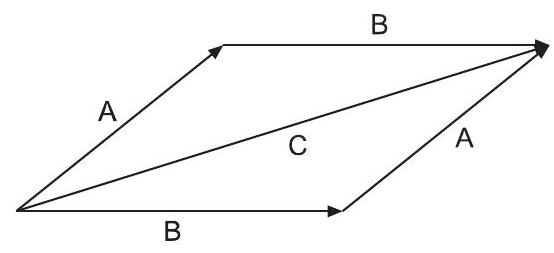
\includegraphics[max width=\textwidth, center]{2024_10_13_e0685a8ee0113ded3493g-47}

Figure 1.7 Addition of two vectors.\\
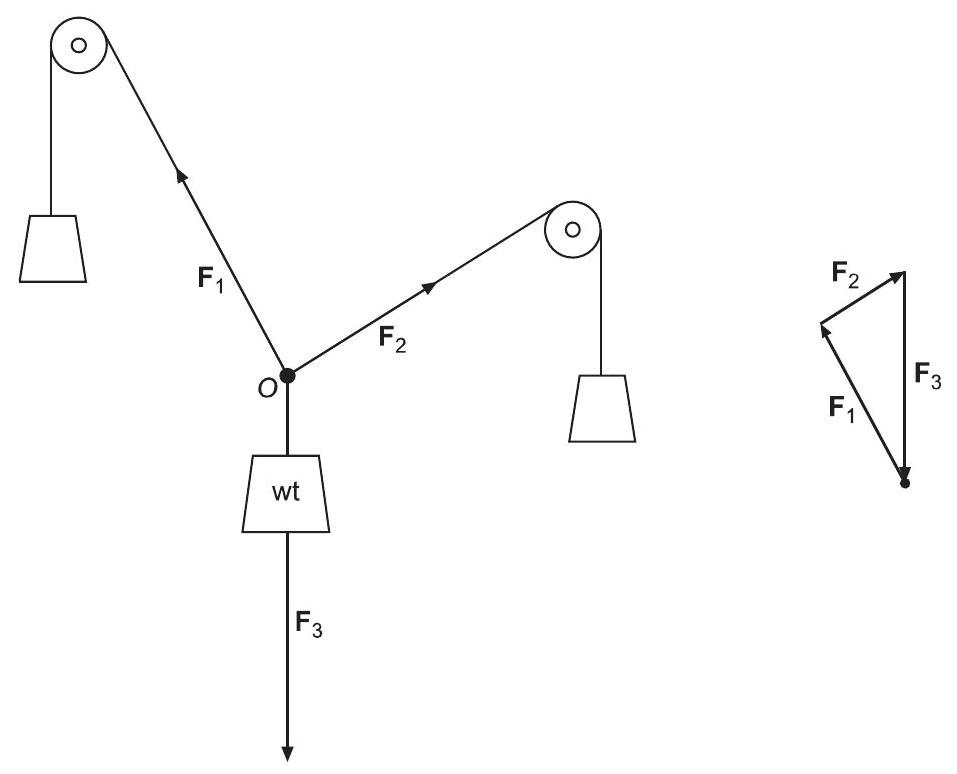
\includegraphics[max width=\textwidth, center]{2024_10_13_e0685a8ee0113ded3493g-48}

Figure 1.8 Equilibrium of forces at the point $O$.\\
now identify $A_{x} \hat{\mathbf{e}}_{x}$ as a vector of signed magnitude $A_{x}$ in the $x$ direction, and we see that A can be represented as the vector sum


\begin{equation*}
\mathbf{A}=A_{x} \hat{\mathbf{e}}_{x}+A_{y} \hat{\mathbf{e}}_{y}+A_{z} \hat{\mathbf{e}}_{z} \tag{1.100}
\end{equation*}


If $\mathbf{A}$ is itself the displacement from the origin to the point $(x, y, z)$, we denote it by the special symbol $\mathbf{r}$ (sometimes called the radius vector), and Eq. (1.100) becomes


\begin{equation*}
\mathbf{r}=x \hat{\mathbf{e}}_{x}+y \hat{\mathbf{e}}_{y}+z \hat{\mathbf{e}}_{z} \tag{1.101}
\end{equation*}


The unit vectors are said to span the space in which our vectors reside, or to form a basis for the space. Either of these statements means that any vector in the space can be constructed as a linear combination of the basis vectors. Since a vector $A$ has specific values of $A_{x}, A_{y}$, and $A_{z}$, this linear combination will be unique.

Sometimes a vector will be specified by its magnitude $A$ and by the angles it makes with the Cartesian coordinate axes. Letting $\alpha, \beta, \gamma$ be the respective angles our vector makes with the $x, y$, and $z$ axes, the components of $\mathbf{A}$ are given by


\begin{equation*}
A_{x}=A \cos \alpha, \quad A_{y}=A \cos \beta, \quad A_{z}=A \cos \gamma \tag{1.102}
\end{equation*}


The quantities $\cos \alpha, \cos \beta, \cos \gamma$ (see Fig. 1.9) are known as the direction cosines of $\mathbf{A}$. Since we already know that $A_{x}^{2}+A_{y}^{2}+A_{z}^{2}=A^{2}$, we see that the direction cosines are not entirely independent, but must satisfy the relation


\begin{equation*}
\cos ^{2} \alpha+\cos ^{2} \beta+\cos ^{2} \gamma=1 \tag{1.103}
\end{equation*}


While the formalism of Eq. (1.100) could be developed with complex values for the components $A_{x}, A_{y}, A_{z}$, the geometric situation being described makes it natural to restrict these coefficients to real values; the space with all possible real values of two coordinates\\
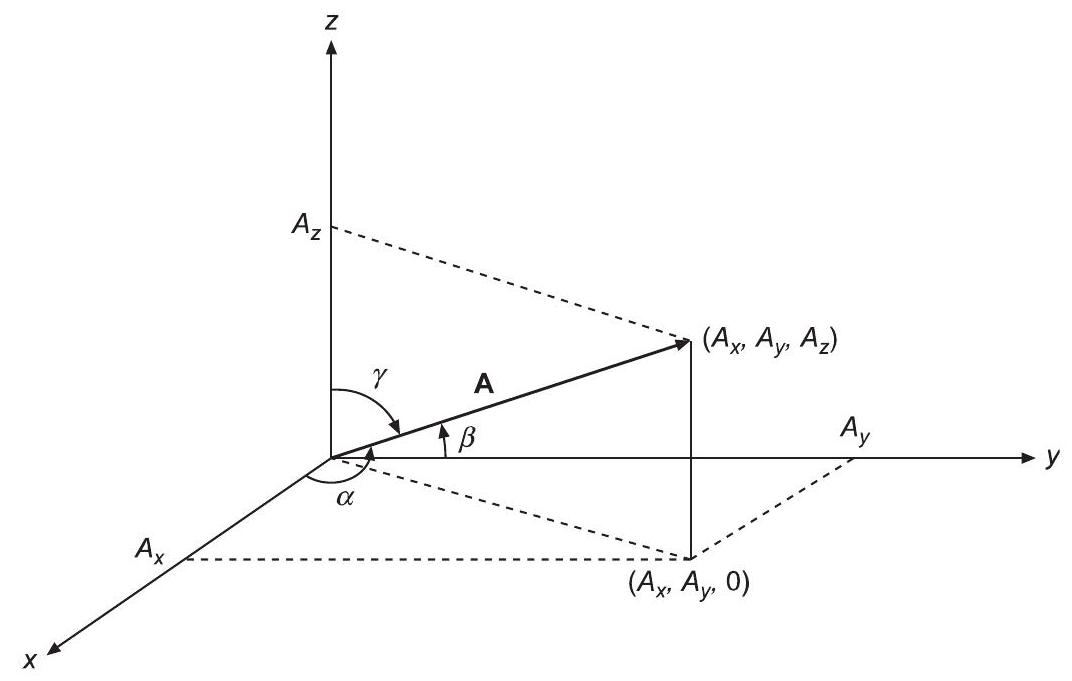
\includegraphics[max width=\textwidth, center]{2024_10_13_e0685a8ee0113ded3493g-49(1)}

Figure 1.9 Cartesian components and direction cosines of $\mathbf{A}$.\\
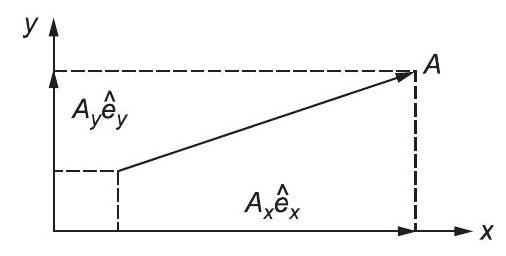
\includegraphics[max width=\textwidth, center]{2024_10_13_e0685a8ee0113ded3493g-49}

Figure 1.10 Projections of $\mathbf{A}$ on the $x$ and $y$ axes.\\
is denoted by mathematicians (and occasionally by us) $\mathbb{R}^{2}$; the complete 3-D space is named $\mathbb{R}^{3}$.

\section*{Dot (Scalar) Product}
When we write a vector in terms of its component vectors in the coordinate directions, as in

$$
\mathbf{A}=A_{x} \hat{\mathbf{e}}_{x}+A_{y} \hat{\mathbf{e}}_{y}+A_{z} \hat{\mathbf{e}}_{z}
$$

we can think of $A_{x} \hat{\mathbf{e}}_{x}$ as its projection in the $x$ direction. Stated another way, it is the portion of $\mathbf{A}$ that is in the subspace spanned by $\hat{\mathbf{e}}_{x}$ alone. The term projection corresponds to the idea that it is the result of collapsing (projecting) a vector onto one of the coordinate axes. See Fig. 1.10.\\
It is useful to define a quantity known as the dot product, with the property that it produces the coefficients, e.g., $A_{x}$, in projections onto the coordinate axes according to


\begin{equation*}
\mathbf{A} \cdot \hat{\mathbf{e}}_{x}=A_{x}=A \cos \alpha, \quad \mathbf{A} \cdot \hat{\mathbf{e}}_{y}=A_{y}=A \cos \beta, \quad \mathbf{A} \cdot \hat{\mathbf{e}}_{z}=A_{z}=A \cos \gamma \tag{1.104}
\end{equation*}


where $\cos \alpha, \cos \beta, \cos \gamma$ are the direction cosines of $\mathbf{A}$.

We want to generalize the notion of the dot product so that it will apply to arbitrary vectors $\mathbf{A}$ and $\mathbf{B}$, requiring that it, like projections, be linear and obey the distributive and associative laws


\begin{align*}
\mathbf{A} \cdot(\mathbf{B}+\mathbf{C}) & =\mathbf{A} \cdot \mathbf{B}+\mathbf{A} \cdot \mathbf{C}  \tag{1.105}\\
\mathbf{A} \cdot(k \mathbf{B}) & =(k \mathbf{A}) \cdot \mathbf{B}=k \mathbf{A} \cdot \mathbf{B} \tag{1.106}
\end{align*}


with $k$ a scalar. Now we can use the decomposition of $\mathbf{B}$ into Cartesian components as in Eq. (1.100), $\mathbf{B}=B_{x} \hat{\mathbf{e}}_{x}+B_{y} \hat{\mathbf{e}}_{y}+B_{z} \hat{\mathbf{e}}_{z}$, to construct the dot product of the vectors $\mathbf{A}$ and B as


\begin{align*}
\mathbf{A} \cdot \mathbf{B} & =\mathbf{A} \cdot\left(B_{x} \hat{\mathbf{e}}_{x}+B_{y} \hat{\mathbf{e}}_{y}+B_{z} \hat{\mathbf{e}}_{z}\right) \\
& =B_{x} \mathbf{A} \cdot \hat{\mathbf{e}}_{x}+B_{y} \mathbf{A} \cdot \hat{\mathbf{e}}_{y}+B_{z} \mathbf{A} \cdot \hat{\mathbf{e}}_{z} \\
& =B_{x} A_{x}+B_{y} A_{y}+B_{z} A_{z} \tag{1.107}
\end{align*}


This leads to the general formula


\begin{equation*}
\mathbf{A} \cdot \mathbf{B}=\sum_{i} B_{i} A_{i}=\sum_{i} A_{i} B_{i}=\mathbf{B} \cdot \mathbf{A} \tag{1.108}
\end{equation*}


which is also applicable when the number of dimensions in the space is other than three. Note that the dot product is commutative, with $\mathbf{A} \cdot \mathbf{B}=\mathbf{B} \cdot \mathbf{A}$.

An important property of the dot product is that $\mathbf{A} \cdot \mathbf{A}$ is the square of the magnitude of A:


\begin{equation*}
\mathbf{A} \cdot \mathbf{A}=A_{x}^{2}+A_{y}^{2}+\cdots=|\mathbf{A}|^{2} \tag{1.109}
\end{equation*}


Applying this observation to $\mathbf{C}=\mathbf{A}+\mathbf{B}$, we have

$$
|\mathbf{C}|^{2}=\mathbf{C} \cdot \mathbf{C}=(\mathbf{A}+\mathbf{B}) \cdot(\mathbf{A}+\mathbf{B})=\mathbf{A} \cdot \mathbf{A}+\mathbf{B} \cdot \mathbf{B}+2 \mathbf{A} \cdot \mathbf{B}
$$

which can be rearranged to


\begin{equation*}
\mathbf{A} \cdot \mathbf{B}=\frac{1}{2}\left[|\mathbf{C}|^{2}-|\mathbf{A}|^{2}-|\mathbf{B}|^{2}\right] \tag{1.110}
\end{equation*}


From the geometry of the vector sum $\mathbf{C}=\mathbf{A}+\mathbf{B}$, as shown in Fig. 1.11, and recalling the law of cosines and its similarity to Eq. (1.110), we obtain the well-known formula


\begin{equation*}
\mathbf{A} \cdot \mathbf{B}=|\mathbf{A}||\mathbf{B}| \cos \theta \tag{1.111}
\end{equation*}


\begin{center}
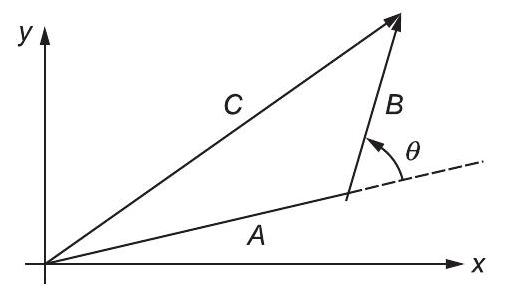
\includegraphics[max width=\textwidth]{2024_10_13_e0685a8ee0113ded3493g-50}
\end{center}

Figure 1.11 Vector sum, $\mathbf{C}=\mathbf{A}+\mathbf{B}$.\\
where $\theta$ is the angle between the directions of $\mathbf{A}$ and $\mathbf{B}$. In contrast with the algebraic formula Eq. (1.108), Eq. (1.111) is a geometric formula for the dot product, and shows clearly that it depends only on the relative directions of $\mathbf{A}$ and $\mathbf{B}$ and is therefore independent of the coordinate system. For that reason the dot product is sometimes also identified as a scalar product.\\
Equation (1.111) also permits an interpretation in terms of the projection of a vector $\mathbf{A}$ in the direction of $\mathbf{B}$ or the reverse. If $\hat{\mathbf{b}}$ is a unit vector in the direction of $\mathbf{B}$, the projection of $A$ in that direction is given by


\begin{equation*}
A_{b} \hat{\mathbf{b}}=(\hat{\mathbf{b}} \cdot \mathbf{A}) \hat{\mathbf{b}}=(A \cos \theta) \hat{\mathbf{b}} \tag{1.112}
\end{equation*}


where $\theta$ is the angle between $\mathbf{A}$ and $\mathbf{B}$. Moreover, the dot product $\mathbf{A} \cdot \mathbf{B}$ can then be identified as $|\mathbf{B}|$ times the magnitude of the projection of $\mathbf{A}$ in the $\mathbf{B}$ direction, so $\mathbf{A} \cdot \mathbf{B}=A_{b} B$. Equivalently, $\mathbf{A} \cdot \mathbf{B}$ is equal to $|\mathbf{A}|$ times the magnitude of the projection of $\mathbf{B}$ in the $\mathbf{A}$ direction, so we also have $\mathbf{A} \cdot \mathbf{B}=B_{a} A$.\\
Finally, we observe that since $|\cos \theta| \leq 1$, Eq. (1.111) leads to the inequality


\begin{equation*}
|\mathbf{A} \cdot \mathbf{B}| \leq|\mathbf{A}||\mathbf{B}| \text {. } \tag{1.113}
\end{equation*}


The equality in Eq. (1.113) holds only if $\mathbf{A}$ and $\mathbf{B}$ are collinear (in either the same or opposite directions). This is the specialization to physical space of the Schwarz inequality, which we will later develop in a more general context.

\section*{Orthogonality}
Equation (1.111) shows that $\mathbf{A} \cdot \mathbf{B}$ becomes zero when $\cos \theta=0$, which occurs at $\theta= \pm \pi / 2$ (i.e., at $\theta= \pm 90^{\circ}$ ). These values of $\theta$ correspond to $\mathbf{A}$ and $\mathbf{B}$ being perpendicular, the technical term for which is orthogonal. Thus,

\section*{$\mathbf{A}$ and $\mathbf{B}$ are orthogonal if and only if $\mathbf{A} \cdot \mathbf{B}=0$.}
Checking this result for two dimensions, we note that $\mathbf{A}$ and $\mathbf{B}$ are perpendicular if the slope of $\mathbf{B}, B_{y} / B_{x}$, is the negative of the reciprocal of $A_{y} / A_{x}$, or

$$
\frac{B_{y}}{B_{x}}=-\frac{A_{x}}{A_{y}}
$$

This result expands to $A_{x} B_{x}+A_{y} B_{y}=0$, the condition that $\mathbf{A}$ and $\mathbf{B}$ be orthogonal.\\
In terms of projections, $\mathbf{A} \cdot \mathbf{B}=0$ means that the projection of $\mathbf{A}$ in the $\mathbf{B}$ direction vanishes (and vice versa). That is of course just another way of saying that $\mathbf{A}$ and $\mathbf{B}$ are orthogonal.\\
The fact that the Cartesian unit vectors are mutually orthogonal makes it possible to simplify many dot product computations. Because


\begin{equation*}
\hat{\mathbf{e}}_{x} \cdot \hat{\mathbf{e}}_{y}=\hat{\mathbf{e}}_{x} \cdot \hat{\mathbf{e}}_{z}=\hat{\mathbf{e}}_{y} \cdot \hat{\mathbf{e}}_{z}=0, \quad \hat{\mathbf{e}}_{x} \cdot \hat{\mathbf{e}}_{x}=\hat{\mathbf{e}}_{y} \cdot \hat{\mathbf{e}}_{y}=\hat{\mathbf{e}}_{z} \cdot \hat{\mathbf{e}}_{z}=1 \tag{1.114}
\end{equation*}


we can evaluate $\mathbf{A} \cdot \mathbf{B}$ as

$$
\begin{gathered}
\left(A_{x} \hat{\mathbf{e}}_{x}+A_{y} \hat{\mathbf{e}}_{y}+A_{z} \hat{\mathbf{e}}_{z}\right) \cdot\left(B_{x} \hat{\mathbf{e}}_{x}+B_{y} \hat{\mathbf{e}}_{y}+B_{z} \hat{\mathbf{e}}_{z}\right)=A_{x} B_{x} \hat{\mathbf{e}}_{x} \cdot \hat{\mathbf{e}}_{x}+A_{y} B_{y} \hat{\mathbf{e}}_{y} \cdot \hat{\mathbf{e}}_{y}+A_{z} B_{z} \hat{\mathbf{e}}_{z} \cdot \hat{\mathbf{e}}_{z} \\
+\left(A_{x} B_{y}+A_{y} B_{x}\right) \hat{\mathbf{e}}_{x} \cdot \hat{\mathbf{e}}_{y}+\left(A_{x} B_{z}+A_{z} B_{x}\right) \hat{\mathbf{e}}_{x} \cdot \hat{\mathbf{e}}_{z}+\left(A_{y} B_{z}+A_{z} B_{y}\right) \hat{\mathbf{e}}_{y} \cdot \hat{\mathbf{e}}_{z} \\
=A_{x} B_{x}+A_{y} B_{y}+A_{z} B_{z}
\end{gathered}
$$

See Chapter 3: Vector Analysis, Section 3.2: Vectors in 3-D Space for an introduction of the cross product of vectors, needed early in Chapter 2.

\section*{Exercises}
1.7.1 The vector $\mathbf{A}$ whose magnitude is 1.732 units makes equal angles with the coordinate axes. Find $A_{x}, A_{y}$, and $A_{z}$.\\
1.7.2 A triangle is defined by the vertices of three vectors $\mathbf{A}, \mathbf{B}$ and $\mathbf{C}$ that extend from the origin. In terms of $\mathbf{A}, \mathbf{B}$, and $\mathbf{C}$ show that the vector sum of the successive sides of the triangle $(A B+B C+C A)$ is zero, where the side $A B$ is from $A$ to $B$, etc.\\
1.7.3 A sphere of radius $a$ is centered at a point $\mathbf{r}_{1}$.\\
(a) Write out the algebraic equation for the sphere.\\
(b) Write out a vector equation for the sphere.

$$
\text { ANS. (a) } \quad\left(x-x_{1}\right)^{2}+\left(y-y_{1}\right)^{2}+\left(z-z_{1}\right)^{2}=a^{2}
$$

(b) $\mathbf{r}=\mathbf{r}_{1}+\mathbf{a}$, where a takes on all directions but has a fixed magnitude $a$.\\
1.7.4 Hubble's law. Hubble found that distant galaxies are receding with a velocity proportional to their distance from where we are on Earth. For the $i$ th galaxy,

$$
\mathbf{v}_{i}=H_{0} \mathbf{r}_{i}
$$

with us at the origin. Show that this recession of the galaxies from us does not imply that we are at the center of the universe. Specifically, take the galaxy at $\mathbf{r}_{1}$ as a new origin and show that Hubble's law is still obeyed.\\
1.7.5 Find the diagonal vectors of a unit cube with one corner at the origin and its three sides lying along Cartesian coordinates axes. Show that there are four diagonals with length $\sqrt{3}$. Representing these as vectors, what are their components? Show that the diagonals of the cube's faces have length $\sqrt{2}$ and determine their components.\\
1.7.6 The vector $\mathbf{r}$, starting at the origin, terminates at and specifies the point in space $(x, y, z)$. Find the surface swept out by the tip of $\mathbf{r}$ if\\
(a) $(\mathbf{r}-\mathbf{a}) \cdot \mathbf{a}=0$. Characterize a geometrically.\\
(b) $(\mathbf{r}-\mathbf{a}) \cdot \mathbf{r}=0$. Describe the geometric role of $\mathbf{a}$.

The vector a is constant (in magnitude and direction).\\
1.7.7 A pipe comes diagonally down the south wall of a building, making an angle of $45^{\circ}$ with the horizontal. Coming into a corner, the pipe turns and continues diagonally down a west-facing wall, still making an angle of $45^{\circ}$ with the horizontal. What is the angle between the south-wall and west-wall sections of the pipe?

ANS. $120^{\circ}$.\\
1.7.8 Find the shortest distance of an observer at the point $(2,1,3)$ from a rocket in free flight with velocity $(1,2,3) \mathrm{km} / \mathrm{s}$. The rocket was launched at time $t=0$ from $(1,1,1)$. Lengths are in kilometers.\\
1.7.9 Show that the medians of a triangle intersect in the center which is $2 / 3$ of the median's length from each vertex. Construct a numerical example and plot it.\\
1.7.10 Prove the law of cosines starting from $\mathbf{A}^{2}=(\mathbf{B}-\mathbf{C})^{2}$.\\
1.7.11 Given the three vectors,

$$
\begin{aligned}
& \mathbf{P}=3 \hat{\mathbf{e}}_{x}+2 \hat{\mathbf{e}}_{y}-\hat{\mathbf{e}}_{z} \\
& \mathbf{Q}=-6 \hat{\mathbf{e}}_{x}-4 \hat{\mathbf{e}}_{y}+2 \hat{\mathbf{e}}_{z} \\
& \mathbf{R}=\hat{\mathbf{e}}_{x}-2 \hat{\mathbf{e}}_{y}-\hat{\mathbf{e}}_{z}
\end{aligned}
$$

find two that are perpendicular and two that are parallel or antiparallel.

\subsection*{1.8 COMPLEX NUMBERS AND FUNCTIONS}
Complex numbers and analysis based on complex variable theory have become extremely important and valuable tools for the mathematical analysis of physical theory. Though the results of the measurement of physical quantities must, we firmly believe, ultimately be described by real numbers, there is ample evidence that successful theories predicting the results of those measurements require the use of complex numbers and analysis. In a later chapter we explore the fundamentals of complex variable theory. Here we introduce complex numbers and identify some of their more elementary properties.

\section*{Basic Properties}
A complex number is nothing more than an ordered pair of two real numbers, $(a, b)$. Similarly, a complex variable is an ordered pair of two real variables,


\begin{equation*}
z \equiv(x, y) \tag{1.115}
\end{equation*}


The ordering is significant. In general $(a, b)$ is not equal to $(b, a)$ and $(x, y)$ is not equal to $(y, x)$. As usual, we continue writing a real number $(x, 0)$ simply as $x$, and we call $i \equiv(0,1)$ the imaginary unit. All of complex analysis can be developed in terms of ordered pairs of numbers, variables, and functions $(u(x, y), v(x, y))$.

We now define addition of complex numbers in terms of their Cartesian components as


\begin{equation*}
z_{1}+z_{2}=\left(x_{1}, y_{1}\right)+\left(x_{2}, y_{2}\right)=\left(x_{1}+x_{2}, y_{1}+y_{2}\right) \tag{1.116}
\end{equation*}


Multiplication of complex numbers is defined as


\begin{equation*}
z_{1} z_{2}=\left(x_{1}, y_{1}\right) \cdot\left(x_{2}, y_{2}\right)=\left(x_{1} x_{2}-y_{1} y_{2}, x_{1} y_{2}+x_{2} y_{1}\right) \tag{1.117}
\end{equation*}


It is obvious that multiplication is not just the multiplication of corresponding components. Using Eq. (1.117) we verify that $i^{2}=(0,1) \cdot(0,1)=(-1,0)=-1$, so we can also identify $i=\sqrt{-1}$ as usual, and further rewrite Eq. (1.115) as


\begin{equation*}
z=(x, y)=(x, 0)+(0, y)=x+(0,1) \cdot(y, 0)=x+i y \tag{1.118}
\end{equation*}


Clearly, introduction of the symbol $i$ is not necessary here, but it is convenient, in large part because the addition and multiplication rules for complex numbers are consistent with those for ordinary arithmetic with the additional property that $i^{2}=-1$ :

$$
\left(x_{1}+i y_{1}\right)\left(x_{2}+i y_{2}\right)=x_{1} x_{2}+i^{2} y_{1} y_{2}+i\left(x_{1} y_{2}+y_{1} x_{2}\right)=\left(x_{1} x_{2}-y_{1} y_{2}\right)+i\left(x_{1} y_{2}+y_{1} x_{2}\right)
$$

in agreement with Eq. (1.117). For historical reasons, $i$ and its multiples are known as imaginary numbers.

The space of complex numbers, sometimes denoted $\mathcal{Z}$ by mathematicians, has the following formal properties:

\begin{itemize}
  \item It is closed under addition and multiplication, meaning that if two complex numbers are added or multiplied, the result is also a complex number.
  \item It has a unique zero number, which when added to any complex number leaves it unchanged and which, when multiplied with any complex number yields zero.
  \item It has a unique unit number, 1 , which when multiplied with any complex number leaves it unchanged.
  \item Every complex number $z$ has an inverse under addition (known as $-z$ ), and every nonzero $z$ has an inverse under multiplication, denoted $z^{-1}$ or $1 / z$.
  \item It is closed under exponentiation: if $u$ and $v$ are complex numbers $u^{v}$ is also a complex number.
\end{itemize}

From a rigorous mathematical viewpoint, the last statement above is somewhat loose, as it does not really define exponentiation, but we will find it adequate for our purposes.

Some additional definitions and properties include the following:\\
Complex conjugation: Like all complex numbers, $i$ has an inverse under addition, denoted $-i$, in two-component form, $(0,-1)$. Given a complex number $z=x+i y$, it is useful to define another complex number, $z^{*}=x-i y$, which we call the complex conjugate of $z .{ }^{6}$ Forming


\begin{equation*}
z z^{*}=(x+i y)(x-i y)=x^{2}+y^{2} \tag{1.119}
\end{equation*}


we see that $z z^{*}$ is real; we define the absolute value of $z$, denoted $|z|$, as $\sqrt{z z^{*}}$.

\footnotetext{${ }^{6}$ The complex conjugate of $z$ is often denoted $\bar{z}$ in the mathematical literature.
}Division: Consider now the division of two complex numbers: $z^{\prime} / z$. We need to manipulate this quantity to bring it to the complex number form $u+i v$ (with $u$ and $v$ real). We may do so as follows:

$$
\frac{z^{\prime}}{z}=\frac{z^{\prime} z^{*}}{z z^{*}}=\frac{\left(x^{\prime}+i y^{\prime}\right)(x-i y)}{x^{2}+y^{2}}
$$

or


\begin{equation*}
\frac{x^{\prime}+i y^{\prime}}{x+i y}=\frac{x x^{\prime}+y y^{\prime}}{x^{2}+y^{2}}+i \frac{x y^{\prime}-x^{\prime} y}{x^{2}+y^{2}} \tag{1.120}
\end{equation*}


\section*{Functions in the Complex Domain}
Since the fundamental operations in the complex domain obey the same rules as those for arithmetic in the space of real numbers, it is natural to define functions so that their real and complex incarnations are similar, and specifically so that the complex and real definitions agree when both are applicable. This means, among other things, that if a function is represented by a power series, we should, within the region of convergence of the power series, be able to use such series with complex values of the expansion variable. This notion is called permanence of the algebraic form.

Applying this concept to the exponential, we define


\begin{equation*}
e^{z}=1+z+\frac{1}{2!} z^{2}+\frac{1}{3!} z^{3}+\frac{1}{4!} z^{4}+\cdots \tag{1.121}
\end{equation*}


Now, replacing $z$ by $i z$, we have


\begin{align*}
e^{i z} & =1+i z+\frac{1}{2!}(i z)^{2}+\frac{1}{3!}(i z)^{3}+\frac{1}{4!}(i z)^{4}+\cdots \\
& =\left[1-\frac{1}{2!} z^{2}+\frac{1}{4!} z^{4}-\cdots\right]+i\left[z-\frac{1}{3!} z^{3}+\frac{1}{5!} z^{5}-\cdots\right] \tag{1.122}
\end{align*}


It was permissible to regroup the terms in the series of Eq. (1.122) because that series is absolutely convergent for all $z$; the d'Alembert ratio test succeeds for all $z$, real or complex. If we now identify the bracketed expansions in the last line of Eq. (1.122) as $\cos z$ and $\sin z$, we have the extremely valuable result


\begin{equation*}
e^{i z}=\cos z+i \sin z \tag{1.123}
\end{equation*}


This result is valid for all $z$, real, imaginary, or complex, but is particularly useful when $z$ is real.

Any function $w(z)$ of a complex variable $z=x+i y$ can in principle be divided into its real and imaginary parts, just as we did when we added, multiplied, or divided complex numbers. That is, we can write


\begin{equation*}
w(z)=u(x, y)+i v(x, y) \tag{1.124}
\end{equation*}


in which the separate functions $u(x, y)$ and $v(x, y)$ are pure real. For example, if $f(z)=z^{2}$, we have

$$
f(z)=(z+i y)^{2}=\left(x^{2}-y^{2}\right)+i(2 x y)
$$

The real part of a function $f(z)$ will be labeled $\mathfrak{R e} f(z)$, whereas the imaginary part will be labeled $\mathfrak{I m} f(z)$. In Eq. (1.124),

$$
\mathfrak{R e} w(z)=u(x, y), \quad \Im \mathfrak{m} w(z)=v(x, y)
$$

The complex conjugate of our function $w(z)$ is $u(x, y)-i v(x, y)$, and depending on $w$, may or may not be equal to $w\left(z^{*}\right)$.

\section*{Polar Representation}
We may visualize complex numbers by assigning them locations on a planar graph, called an Argand diagram or, more colloquially, the complex plane. Traditionally the real component is plotted horizontally, on what is called the real axis, with the imaginary axis in the vertical direction. See Fig. 1.12. An alternative to identifying points by their Cartesian coordinates $(x, y)$ is to use polar coordinates $(r, \theta)$, with


\begin{equation*}
x=r \cos \theta, \quad y=r \sin \theta, \quad \text { or } \quad r=\sqrt{x^{2}+y^{2}}, \quad \theta=\tan ^{-1} y / x \tag{1.125}
\end{equation*}


The $\arctan$ function $\tan ^{-1}(y / x)$ is multiple valued; the correct location on an Argand diagram needs to be consistent with the individual values of $x$ and $y$.

The Cartesian and polar representations of a complex number can also be related by writing


\begin{equation*}
x+i y=r(\cos \theta+i \sin \theta)=r e^{i \theta} \tag{1.126}
\end{equation*}


where we have used Eq. (1.123) to introduce the complex exponential. Note that $r$ is also $|z|$, so the magnitude of $z$ is given by its distance from the origin in an Argand diagram. In complex variable theory, $r$ is also called the modulus of $z$ and $\theta$ is termed the argument or the phase of $z$.

If we have two complex numbers, $z$ and $z^{\prime}$, in polar form, their product $z z^{\prime}$ can be written


\begin{equation*}
z z^{\prime}=\left(r e^{i \theta}\right)\left(r^{\prime} e^{i \theta^{\prime}}\right)=\left(r r^{\prime}\right) e^{i\left(\theta+\theta^{\prime}\right)} \tag{1.127}
\end{equation*}


showing that the location of the product in an Argand diagram will have argument (polar angle) at the sum of the polar angles of the factors, and with a magnitude that is the product\\
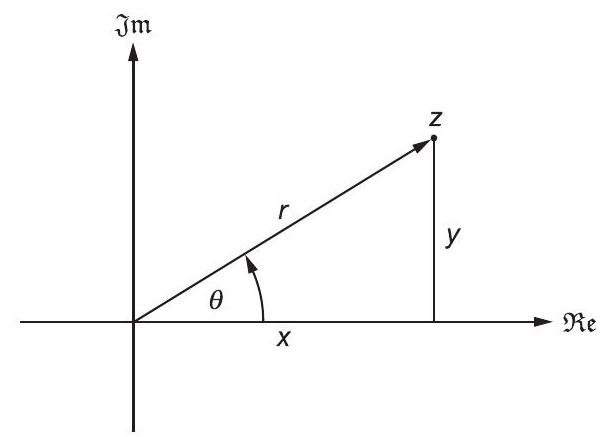
\includegraphics[max width=\textwidth, center]{2024_10_13_e0685a8ee0113ded3493g-56}

Figure 1.12 Argand diagram, showing location of $z=x+i y=r e^{i \theta}$.\\
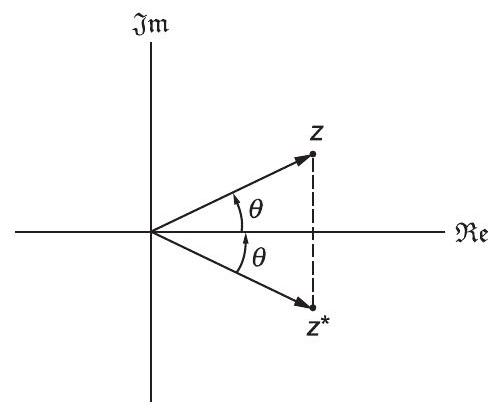
\includegraphics[max width=\textwidth, center]{2024_10_13_e0685a8ee0113ded3493g-57(1)}\\
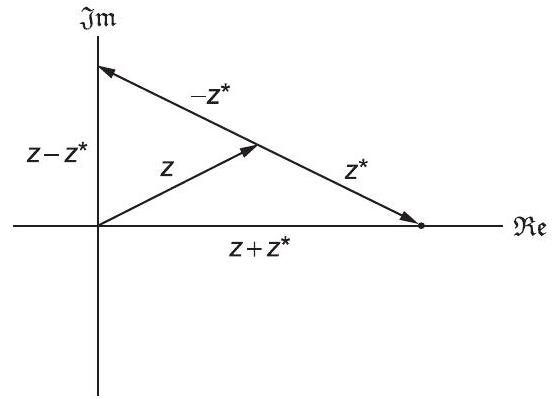
\includegraphics[max width=\textwidth, center]{2024_10_13_e0685a8ee0113ded3493g-57}

Figure 1.13 Left: Relation of $z$ and $z^{*}$. Right: $z+z^{*}$ and $z-z^{*}$.\\
of their magnitudes. Conversely, the quotient $z / z^{\prime}$ will have magnitude $r / r^{\prime}$ and argument $\theta-\theta^{\prime}$. These relationships should aid in getting a qualitative understanding of complex multiplication and division. This discussion also shows that multiplication and division are easier in the polar representation, whereas addition and subtraction have simpler forms in Cartesian coordinates.\\
The plotting of complex numbers on an Argand diagram makes obvious some other properties. Since addition on an Argand diagram is analogous to 2-D vector addition, it can be seen that


\begin{equation*}
\left||z|-\left|z^{\prime}\right|\right| \leq\left|z \pm z^{\prime}\right| \leq|z|+\left|z^{\prime}\right| \tag{1.128}
\end{equation*}


Also, since $z^{*}=r e^{-i \theta}$ has the same magnitude as $z$ but an argument that differs only in sign, $z+z^{*}$ will be real and equal to $2 \mathfrak{R e} z$, while $z-z^{*}$ will be pure imaginary and equal to $2 i \mathfrak{I m} z$. See Fig. 1.13 for an illustration of this discussion.

We can use an Argand diagram to plot values of a function $w(z)$ as well as just $z$ itself, in which case we could label the axes $u$ and $v$, referring to the real and imaginary parts of $w$. In that case, we can think of the function $w(z)$ as providing a mapping from the $x y$ plane to the $u v$ plane, with the effect that any curve in the $x y$ (sometimes called $z$ ) plane is mapped into a corresponding curve in the $u v(=w)$ plane. In addition, the statements of the preceding paragraph can be extended to functions:


\begin{gather*}
\left||w(z)|-\left|w^{\prime}(z)\right|\right| \leq\left|w(z) \pm w^{\prime}(z)\right| \leq|w(z)|+\left|w^{\prime}(z)\right| \\
\mathfrak{R e} w(z)=\frac{w(z)+[w(z)]^{*}}{2}, \quad \Im \mathfrak{m} w(z)=\frac{w(z)-[w(z)]^{*}}{2} \tag{1.129}
\end{gather*}


\section*{Complex Numbers of Unit Magnitude}
Complex numbers of the form


\begin{equation*}
e^{i \theta}=\cos \theta+i \sin \theta \tag{1.130}
\end{equation*}


where we have given the variable the name $\theta$ to emphasize the fact that we plan to restrict it to real values, correspond on an Argand diagram to points for which $x=\cos \theta, y=\sin \theta$,\\
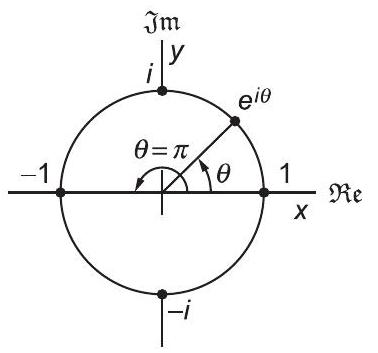
\includegraphics[max width=\textwidth, center]{2024_10_13_e0685a8ee0113ded3493g-58}

Figure 1.14 Some values of $z$ on the unit circle.\\
and whose magnitude is therefore $\cos ^{2} \theta+\sin ^{2} \theta=1$. The points $\exp (i \theta)$ therefore lie on the unit circle, at polar angle $\theta$. This observation makes obvious a number of relations that could in principle also be deduced from Eq. (1.130). For example, if $\theta$ has the special values $\pi / 2$, $\pi$, or $3 \pi / 2$, we have the interesting relationships


\begin{equation*}
e^{i \pi / 2}=i, \quad e^{i \pi}=-1, \quad e^{3 i \pi / 2}=-i \tag{1.131}
\end{equation*}


We also see that $\exp (i \theta)$ is periodic, with period $2 \pi$, so


\begin{equation*}
e^{2 i \pi}=e^{4 i \pi}=\cdots=1, \quad e^{3 i \pi / 2}=e^{-i \pi / 2}=-i, \text { etc. } \tag{1.132}
\end{equation*}


A few relevant values of $z$ on the unit circle are illustrated in Fig. 1.14. These relationships cause the real part of $\exp (i \omega t)$ to describe oscillation at angular frequency $\omega$, with $\exp (i[\omega t+\delta])$ describing an oscillation displaced from that first mentioned by a phase difference $\delta$.

\section*{Circular and Hyperbolic Functions}
The relationship encapsulated in Eq. (1.130) enables us to obtain convenient formulas for the sine and cosine. Taking the sum and difference of $\exp (+i \theta)$ and $\exp (-i \theta)$, we have


\begin{equation*}
\cos \theta=\frac{e^{i \theta}+e^{-i \theta}}{2}, \quad \sin \theta=\frac{e^{i \theta}-e^{-i \theta}}{2 i} \tag{1.133}
\end{equation*}


These formulas place the definitions of the hyperbolic functions in perspective:


\begin{equation*}
\cosh \theta=\frac{e^{\theta}+e^{-\theta}}{2}, \quad \sinh \theta=\frac{e^{\theta}-e^{-\theta}}{2} \tag{1.134}
\end{equation*}


Comparing these two sets of equations, it is possible to establish the formulas


\begin{equation*}
\cosh i z=\cos z, \quad \sinh i z=i \sin z \tag{1.135}
\end{equation*}


Proof is left to Exercise 1.8.5.\\
The fact that $\exp (\operatorname{in} \theta)$ can be written in the two equivalent forms


\begin{equation*}
\cos n \theta+i \sin n \theta=(\cos \theta+i \sin \theta)^{n} \tag{1.136}
\end{equation*}


establishes a relationship known as de Moivre's Theorem. By expanding the right member of Eq. (1.136), we easily obtain trigonometric multiple-angle formulas, of which the simplest examples are the well-known results

$$
\sin (2 \theta)=2 \sin \theta \cos \theta, \quad \cos (2 \theta)=\cos ^{2} \theta-\sin ^{2} \theta
$$

If we solve the $\sin \theta$ formula of Eq. (1.133) for $\exp (i \theta)$, we get (choosing the plus sign for the radical)

$$
e^{i \theta}=i \sin \theta+\sqrt{1-\sin ^{2} \theta}
$$

Setting $\sin \theta=z$ and $\theta=\sin ^{-1}(z)$, and taking the logarithm of both sides of the above equation, we express the inverse trigonometric function in terms of logarithms.

$$
\sin ^{-1}(z)=-i \ln \left[i z+\sqrt{1-z^{2}}\right]
$$

The set of formulas that can be generated in this way includes:

\[
\begin{array}{cc}
\sin ^{-1}(z)=-i \ln \left[i z+\sqrt{1-z^{2}}\right], \quad \tan ^{-1}(z)=\frac{i}{2}[\ln (1-i z)-\ln (1+i z)] \\
\sinh ^{-1}(z)=\ln \left[z+\sqrt{1+z^{2}}\right], \quad \tanh ^{-1}(z)=\frac{1}{2}[\ln (1+z)-\ln (1-z)] \tag{1.137}
\end{array}
\]

\section*{Powers and Roots}
The polar form is very convenient for expressing powers and roots of complex numbers. For integer powers, the result is obvious and unique:

$$
z=r e^{i \varphi}, \quad z^{n}=r^{n} e^{i n \varphi}
$$

For roots (fractional powers), we also have

$$
z=r e^{i \varphi}, \quad z^{1 / n}=r^{1 / n} e^{i \varphi / n}
$$

but the result is not unique. If we write $z$ in the alternate but equivalent form

$$
z=r e^{i(\varphi+2 m \pi)}
$$

where $m$ is an integer, we now get additional values for the root:

$$
z^{1 / n}=r^{1 / n} e^{i(\varphi+2 m \pi) / n}, \quad(\text { any integer } m)
$$

If $n=2$ (corresponding to the square root), different choices of $m$ will lead to two distinct values of $z^{1 / 2}$, both of the same modulus but differing in argument by $\pi$. This corresponds to the well-known result that the square root is double-valued and can be written with either sign.\\
In general, $z^{1 / n}$ is $n$-valued, with successive values having arguments that differ by $2 \pi / n$. Figure 1.15 illustrates the multiple values of $1^{1 / 3}, i^{1 / 3}$, and $(-1)^{1 / 3}$.\\
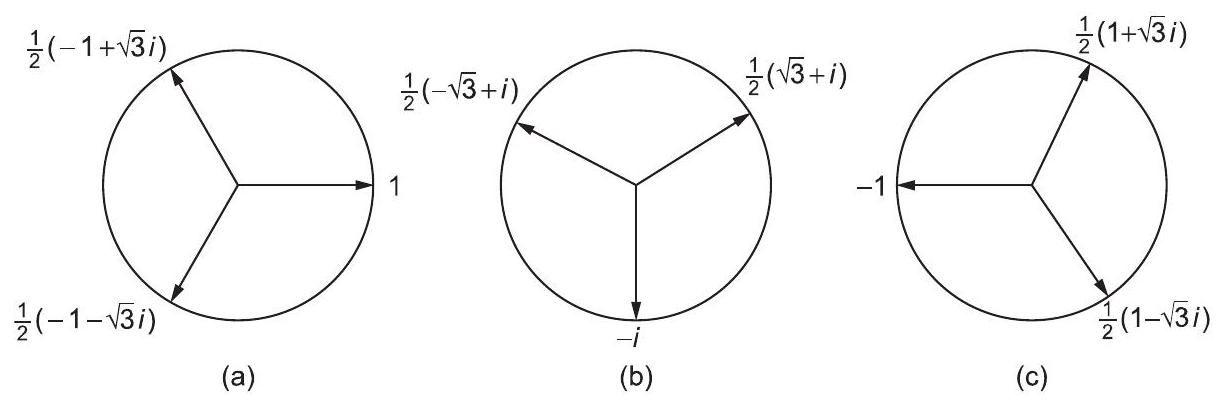
\includegraphics[max width=\textwidth, center]{2024_10_13_e0685a8ee0113ded3493g-60}

Figure 1.15 Cube roots: (a) $1^{1 / 3}$; (b) $i^{1 / 3}$; (c) $(-1)^{1 / 3}$.

\section*{Logarithm}
Another multivalued complex function is the logarithm, which in the polar representation takes the form

$$
\ln z=\ln \left(r e^{i \theta}\right)=\ln r+i \theta
$$

However, it is also true that


\begin{equation*}
\ln z=\ln \left(r e^{i(\theta+2 n \pi)}\right)=\ln r+i(\theta+2 n \pi) \tag{1.138}
\end{equation*}


for any positive or negative integer $n$. Thus, $\ln z$ has, for a given $z$, the infinite number of values corresponding to all possible choices of $n$ in Eq. (1.138).

\section*{Exercises}
1.8.1 Find the reciprocal of $x+i y$, working in polar form but expressing the final result in Cartesian form.\\
1.8.2 Show that complex numbers have square roots and that the square roots are contained in the complex plane. What are the square roots of $i$ ?\\
1.8.3 Show that\\
(a) $\cos n \theta=\cos ^{n} \theta-\binom{n}{2} \cos ^{n-2} \theta \sin ^{2} \theta+\binom{n}{4} \cos ^{n-4} \theta \sin ^{4} \theta-\cdots$,\\
(b) $\sin n \theta=\binom{n}{1} \cos ^{n-1} \theta \sin \theta-\binom{n}{3} \cos ^{n-3} \theta \sin ^{3} \theta+\cdots$\\
1.8.4 Prove that\\
(a) $\sum_{n=0}^{N-1} \cos n x=\frac{\sin (N x / 2)}{\sin x / 2} \cos (N-1) \frac{x}{2}$,\\
(b) $\sum_{n=0}^{N-1} \sin n x=\frac{\sin (N x / 2)}{\sin x / 2} \sin (N-1) \frac{x}{2}$.

These series occur in the analysis of the multiple-slit diffraction pattern.\\
1.8.5 Assume that the trigonometric functions and the hyperbolic functions are defined for complex argument by the appropriate power series. Show that

$$
\begin{aligned}
& i \sin z=\sinh i z, \sin i z=i \sinh z \\
& \cos z=\cosh i z, \cos i z=\cosh z
\end{aligned}
$$

1.8.6 Using the identities

$$
\cos z=\frac{e^{i z}+e^{-i z}}{2}, \quad \sin z=\frac{e^{i z}-e^{-i z}}{2 i}
$$

established from comparison of power series, show that\\
(a) $\sin (x+i y)=\sin x \cosh y+i \cos x \sinh y$\\
$\cos (x+i y)=\cos x \cosh y-i \sin x \sinh y$\\
(b) $|\sin z|^{2}=\sin ^{2} x+\sinh ^{2} y, \quad|\cos z|^{2}=\cos ^{2} x+\sinh ^{2} y$.

This demonstrates that we may have $|\sin z|,|\cos z|>1$ in the complex plane.\\
1.8.7 From the identities in Exercises 1.8 .5 and 1.8 .6 show that\\
(a) $\sinh (x+i y)=\sinh x \cos y+i \cosh x \sin y$, $\cosh (x+i y)=\cosh x \cos y+i \sinh x \sin y$\\
(b) $|\sinh z|^{2}=\sinh ^{2} x+\sin ^{2} y, \quad|\cosh z|^{2}=\cosh ^{2} x+\sin ^{2} y$.\\
1.8.8 Show that\\
(a) $\tanh \frac{z}{2}=\frac{\sinh x+i \sin y}{\cosh x+\cos y}$\\
(b) $\operatorname{coth} \frac{z}{2}=\frac{\sinh x-i \sin y}{\cosh x-\cos y}$.\\
1.8.9 By comparing series expansions, show that $\tan ^{-1} x=\frac{i}{2} \ln \left(\frac{1-i x}{1+i x}\right)$.\\
1.8.10 Find the Cartesian form for all values of\\
(a) $(-8)^{1 / 3}$,\\
(b) $i^{1 / 4}$\\
(c) $e^{i \pi / 4}$.\\
1.8.11 Find the polar form for all values of\\
(a) $(1+i)^{3}$,\\
(b) $(-1)^{1 / 5}$.

\subsection*{1.9 DERIVATIVES AND EXTREMA}
We recall the familiar limit identified as the derivative, $d f(x) / d x$, of a function $f(x)$ at a point $x$ :


\begin{equation*}
\frac{d f(x)}{d x}=\lim _{\varepsilon=0} \frac{f(x+\varepsilon)-f(x)}{\varepsilon} \tag{1.139}
\end{equation*}


the derivative is only defined if the limit exists and is independent of the direction from which $\varepsilon$ approaches zero. The variation or differential of $f(x)$ associated with a change $d x$ in its independent variable from the reference value $x$ assumes the form


\begin{equation*}
d f=f(x+d x)-f(x)=\frac{d f}{d x} d x \tag{1.140}
\end{equation*}


in the limit that $d x$ is small enough that terms dependent on $d x^{2}$ and higher powers of $d x$ become negligible. The mean value theorem (based on the continuity of $f$ ) tells us that here, $d f / d x$ is evaluated at some point $\xi$ between $x$ and $x+d x$, but as $d x \rightarrow 0, \xi \rightarrow x$.

When a quantity of interest is a function of two or more independent variables, the generalization of Eq. (1.140) is (illustrating for the physically important three-variable case):


\begin{align*}
d f= & {[f(x+d x, y+d y, z+d z)-f(x, y+d y, z+d z)] } \\
& +[(f(x, y+d y, z+d z)-f(x, y, z+d z)] \\
& +[f(x, y, z+d z)-f(x, y, z)] \\
= & \frac{\partial f}{\partial x} d x+\frac{\partial f}{\partial y} d y+\frac{\partial f}{\partial z} d z \tag{1.141}
\end{align*}


where the partial derivatives indicate differentiation in which the independent variables not being differentiated are kept fixed. The fact that $\partial f / \partial x$ is evaluated at $y+d y$ and $z+d z$ instead of at $y$ and $z$ alters the derivative by amounts that are of order $d y$ and $d z$, and therefore the change becomes negligible in the limit of small variations. It is thus consistent to interpret Eq. (1.141) as involving partial derivatives that are all evaluated at the reference point $x, y, z$.

Further analysis of the same sort as led to Eq. (1.141) can be used to define higher derivatives and to establish the useful result that cross derivatives (e.g., $\partial^{2} / \partial x \partial y$ ) are independent of the order in which the differentiations are performed:


\begin{equation*}
\frac{\partial}{\partial y}\left(\frac{\partial f}{\partial x}\right) \equiv \frac{\partial^{2} f}{\partial y \partial x}=\frac{\partial^{2} f}{\partial x \partial y} \tag{1.142}
\end{equation*}


Sometimes it is not clear from the context which variables other than that being differentiated are independent, and it is then advisable to attach subscripts to the derivative notation to avoid ambiguity. For example, if $x, y$, and $z$ have been defined in a problem, but only two of them are independent, one might write

$$
\left(\frac{\partial f}{\partial x}\right)_{y} \text { or }\left(\frac{\partial f}{\partial x}\right)_{z}
$$

whichever is actually meant.

For working with functions of several variables, we note two useful formulas that follow from Eq. (1.141):

\begin{enumerate}
  \item The chain rule,
\end{enumerate}


\begin{equation*}
\frac{d f}{d s}=\frac{\partial f}{\partial x} \frac{d x}{d s}+\frac{\partial f}{\partial y} \frac{d y}{d s}+\frac{\partial f}{\partial z} \frac{d z}{d s} \tag{1.143}
\end{equation*}


which applies when $x, y$, and $z$ are functions of another variable, $s$,\\
2. A formula obtained by setting $d f=0$ (here shown for the case where there are only two independent variables and the $d z$ term of Eq. (1.141) is absent):


\begin{equation*}
\left(\frac{\partial y}{\partial x}\right)_{f}=-\frac{\left(\frac{\partial f}{\partial x}\right)_{y}}{\left(\frac{\partial f}{\partial y}\right)_{x}} \tag{1.144}
\end{equation*}


In Lagrangian mechanics, one occasionally encounters expressions such as ${ }^{7}$

$$
\frac{d}{d t} L(x, \dot{x}, t)=\left[\frac{\partial L}{\partial x} \dot{x}+\frac{\partial L}{\partial \dot{x}} \ddot{x}+\frac{\partial L}{\partial t}\right]
$$

an example of use of the chain rule. Here it is necessary to distinguish between the formal dependence of $L$ on its three arguments and the overall dependence of $L$ on time. Note the use of the ordinary $(d / d t)$ and partial $(\partial / \partial t)$ derivative notation.

\section*{Stationary Points}
Whether or not a set of independent variables (e.g., $x, y, z$ of our previous discussion) represents directions in space, one can ask how a function $f$ changes if we move in various directions in the space of the independent variables; the answer is provided by Eq. (1.143), where the "direction" is defined by the values of $d x / d s, d y / d s$, etc.\\
It is often desired to find the minimum of a function $f$ of $n$ variables $x_{i}, i=1, \ldots, n$, and a necessary but not sufficient condition on its position is that

$$
\frac{d f}{d s}=0 \text { for all directions of } d s
$$

This is equivalent to requiring


\begin{equation*}
\frac{\partial f}{\partial x_{i}}=0, \quad i=1, \ldots, n \tag{1.145}
\end{equation*}


All points in the $\left\{x_{i}\right\}$ space that satisfy Eq. (1.145) are termed stationary; for a stationary point of $f$ to be a minimum, it is also necessary that the second derivatives $d^{2} f / d s^{2}$ be positive for all directions of $s$. Conversely, if the second derivatives in all directions are negative, the stationary point is a maximum. If neither of these conditions are satisfied, the stationary point is neither a maximum nor a minimum, and is often called a saddle point because of the appearance of the surface of $f$ when there are two independent variables

\footnotetext{${ }^{7}$ Here dots indicate time derivatives.
}
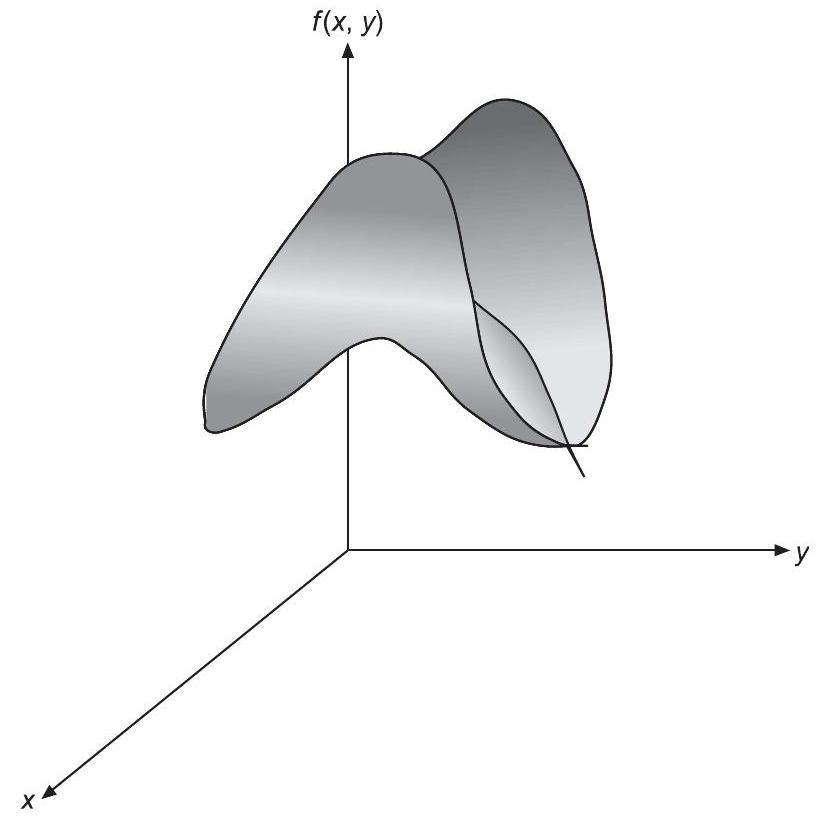
\includegraphics[max width=\textwidth, center]{2024_10_13_e0685a8ee0113ded3493g-64}

Figure 1.16 A stationary point that is neither a maximum nor minimum (a saddle point).\\
(see Fig. 1.16). It is often obvious whether a stationary point is a minimum or maximum, but a complete discussion of the issue is nontrivial.

\section*{Exercises}
19.1 Derive the following formula for the Maclaurin expansion of a function of two variables:

$$
\begin{aligned}
f(x, y)= & f(0,0)+x \frac{\partial f}{\partial x}+y \frac{\partial f}{\partial y} \\
& +\frac{1}{2!}\left[\binom{2}{0} x^{2} \frac{\partial^{2} f}{\partial x^{2}}+\binom{2}{1} x y \frac{\partial^{2} f}{\partial x \partial y}+\binom{2}{2} y^{2} \frac{\partial^{2} f}{\partial y^{2}}\right] \\
& +\frac{1}{3!}\left[\binom{3}{0} x^{3} \frac{\partial^{3} f}{\partial x^{3}}+\binom{3}{1} x^{2} y \frac{\partial^{3} f}{\partial x^{2} \partial y}+\binom{3}{2} x y^{2} \frac{\partial^{3} f}{\partial x \partial y^{2}}+\binom{3}{3} y^{3} \frac{\partial^{3} f}{\partial y^{3}}\right]+\cdots
\end{aligned}
$$

where all the partial derivatives are to be evaluated at the point $(0,0)$.\\
1.9.2 The result in Exercise 1.9.1 can be generalized to larger numbers of independent variables. Prove that for an $m$-variable system, the Maclaurin expansion can be written in\\
the symbolic form

$$
f\left(x_{1}, \ldots, x_{m}\right)=\sum_{n=0}^{\infty} \frac{t^{n}}{n!}\left(\sum_{i=1}^{m} \alpha_{i} \frac{\partial}{\partial x_{i}}\right)^{n} f(0, \ldots, 0)
$$

where in the right-hand side we have made the substitutions $x_{j}=\alpha_{j} t$.

\subsection*{1.10 EVALUATION OF INTEGRALS}
Proficiency in the evaluation of integrals involves a mixture of experience, skill in pattern recognition, and a few tricks. The most familiar include the technique of integration by parts, and the strategy of changing the variable of integration. We review here some methods for integrals in one and multiple dimensions.

\section*{Integration by Parts}
The technique of integration by parts is part of every elementary calculus course, but its use is so frequent and ubiquitous that it bears inclusion here. It is based on the obvious relation, for $u$ and $v$ arbitrary functions of $x$,

$$
d(u v)=u d v+v d u
$$

Integrating both sides of this equation over an interval $(a, b)$, we reach

$$
\left.u v\right|_{a} ^{b}=\int_{a}^{b} u d v+\int_{a}^{b} v d u
$$

which is usually rearranged to the well-known form


\begin{equation*}
\int_{a}^{b} u d v=\left.u v\right|_{a} ^{b}-\int_{a}^{b} v d u \tag{1.146}
\end{equation*}


\section*{Example 1.10.1 INTEGRATION BY PARTS}
Consider the integral $\int_{a}^{b} x \sin x d x$. We identify $u=x$ and $d v=\sin x d x$. Differentiating and integrating, we find $d u=d x$ and $v=-\cos x$, so Eq. (1.146) becomes

$$
\int_{a}^{b} x \sin x d x=\left.(x)(-\cos x)\right|_{a} ^{b}-\int_{a}^{b}(-\cos x) d x=a \cos a-b \cos b+\sin b-\sin a
$$

The key to the effective use of this technique is to see how to partition an integrand into $u$ and $d v$ in a way that makes it easy to form $d u$ and $v$ and also to integrate $\int v d u$.

\section*{Special Functions}
A number of special functions have become important in physics because they arise in frequently encountered situations. Identifying a one-dimensional (1-D) integral as one yielding a special function is almost as good as a straight-out evaluation, in part because it prevents the waste of time that otherwise might be spent trying to carry out the integration. But of perhaps more importance, it connects the integral to the full body of knowledge regarding its properties and evaluation. It is not necessary for every physicist to know everything about all known special functions, but it is desirable to have an overview permitting the recognition of special functions which can then be studied in more detail if necessary.

It is common for a special function to be defined in terms of an integral over the range for which that integral converges, but to have its definition extended to a larger domain

Table 1.2 Special Functions of Importance in Physics

\begin{center}
\begin{tabular}{|c|c|c|}
\hline
Gamma function & \( \Gamma(x)=\int_{0}^{\infty} t^{x-1} e^{-t} d t \) & See Chap. 13. \\
\hline
Factorial ( $n$ integral) & \( n!=\int_{0}^{\infty} t^{n} e^{-t} d t \) & $n!=\Gamma(n+1)$ \\
\hline
Riemann zeta function & \( \zeta(x)=\frac{1}{\Gamma(x)} \int_{0}^{\infty} \frac{t^{x-1} d t}{e^{t}-1} \) & See Chaps. 1 and 12. \\
\hline
Exponential integrals & \( E_{n}(x)=\int_{1}^{\infty} t^{-n} e^{-t} d t \) & $E_{1}(x) \equiv-\operatorname{Ei}(-x)$ \\
\hline
Sine integral & \( \operatorname{si}(x)=-\int_{x}^{\infty} \frac{\sin t}{t} d t \) &  \\
\hline
Cosine integral & \( \operatorname{Ci}(x)=-\int_{x}^{\infty} \frac{\cos t}{t} d t \) &  \\
\hline
Error functions & \( \operatorname{erf}(x)=\frac{2}{\sqrt{\pi}} \int_{0}^{x} e^{-t^{2}} d t \) & $\operatorname{erf}(\infty)=1$ \\
\hline
 & \( \operatorname{erfc}(x)=\frac{2}{\sqrt{\pi}} \int_{x}^{\infty} e^{-t^{2}} d t \) & $\operatorname{erfc}(x)=1-\operatorname{erf}(x)$ \\
\hline
Dilogarithm & \( \mathrm{Li}_{2}(x)=-\int_{0}^{x} \frac{\ln (1-t)}{t} d t \) &  \\
\hline
\end{tabular}
\end{center}

by analytic continuation in the complex plane (cf. Chapter 11) or by the establishment of suitable functional relations. We present in Table 1.2 only the most useful integral representations of a few functions of frequent occurrence. More detail is provided by a variety of on-line sources and in material listed under Additional Readings at the end of this chapter, particularly the compilations by Abramowitz and Stegun and by Gradshteyn and Ryzhik.\\
A conspicuous omission from the list in Table 1.2 is the extensive family of Bessel functions. A short table cannot suffice to summarize their numerous integral representations; a survey of this topic is in Chapter 14. Other important functions in more than one variable or with indices in addition to arguments have also been omitted from the table.

\section*{Other Methods}
An extremely powerful method for the evaluation of definite integrals is that of contour integration in the complex plane. This method is presented in Chapter 11 and will not be discussed here.\\
Integrals can often be evaluated by methods that involve integration or differentiation with respect to parameters, thereby obtaining relations between known integrals and those whose values are being sought.

\section*{Example 1.10.2 Differentiate Parameter}
We wish to evaluate the integral

$$
I=\int_{0}^{\infty} \frac{e^{-x^{2}}}{x^{2}+a^{2}} d x
$$

We introduce a parameter, $t$, to facilitate further manipulations, and consider the related integral

$$
J(t)=\int_{0}^{\infty} \frac{e^{-t\left(x^{2}+a^{2}\right)}}{x^{2}+a^{2}} d x
$$

we note that $I=e^{a^{2}} J(1)$.\\
We now differentiate $J(t)$ with respect to $t$ and evaluate the resulting integral, which is a scaled version of Eq. (1.148):


\begin{equation*}
\frac{d J(t)}{d t}=-\int_{0}^{\infty} e^{-t\left(x^{2}+a^{2}\right)} d x=-e^{-t a^{2}} \int_{0}^{\infty} e^{-t x^{2}} d x=-\frac{1}{2} \sqrt{\frac{\pi}{t}} e^{-t a^{2}} \tag{1.147}
\end{equation*}


To recover $J(t)$ we integrate Eq. (1.147) between $t$ and $\infty$, making use of the fact that $J(\infty)=0$. To carry out the integration it is convenient to make the substitution $u^{2}=a^{2} t$,\\
so we get

$$
J(t)=\frac{\sqrt{\pi}}{2} \int_{t}^{\infty} \frac{e^{-t a^{2}}}{t^{1 / 2}} d t=\frac{\sqrt{\pi}}{a} \int_{a t^{1 / 2}}^{\infty} e^{-u^{2}} d u
$$

which we now recognize as $J(t)=(\pi / 2 a) \operatorname{erfc}\left(a t^{1 / 2}\right)$. Thus, our final result is

$$
I=\frac{\pi}{2 a} e^{a^{2}} \operatorname{erfc}(a)
$$

Many integrals can be evaluated by first converting them into infinite series, then manipulating the resulting series, and finally either evaluating the series or recognizing it as a special function.

\section*{Example 1.10.3 Expand, Then InteGRATe}
Consider $I=\int_{0}^{1} \frac{d x}{x} \ln \left(\frac{1+x}{1-x}\right)$. Using Eq. (1.120) for the logarithm,

$$
I=\int_{0}^{1} d x 2\left[1+\frac{x^{2}}{3}+\frac{x^{4}}{5}+\cdots\right]=2\left[1+\frac{1}{3^{2}}+\frac{1}{5^{2}}+\cdots\right]
$$

Noting that

$$
\frac{1}{2^{2}} \zeta(2)=\frac{1}{2^{2}}+\frac{1}{4^{2}}+\frac{1}{6^{2}}+\cdots
$$

we see that

$$
\zeta(2)-\frac{1}{4} \zeta(2)=1+\frac{1}{3^{2}}+\frac{1}{5^{2}}+\cdots
$$

so $I=\frac{3}{2} \zeta(2)$.\\
Simply using complex numbers aids in the evaluation of some integrals. Take, for example, the elementary integral

$$
I=\int \frac{d x}{1+x^{2}}
$$

Making a partial fraction decomposition of $\left(1+x^{2}\right)^{-1}$ and integrating, we easily get

$$
I=\int \frac{1}{2}\left[\frac{1}{1+i x}+\frac{1}{1-i x}\right] d x=\frac{i}{2}[\ln (1-i x)-\ln (1+i x)]
$$

From Eq. (1.137), we recognize this as $\tan ^{-1}(x)$.\\
The complex exponential forms of the trigonometric functions provide interesting approaches to the evaluation of certain integrals. Here is an example.

\section*{Example 1.10.4 A TrigoNOMETRIC INTEGRAL}
Consider $\quad I=\int_{0}^{\infty} e^{-a t} \cos b t d t$,\\
where $a$ and $b$ are real and positive. Because $\cos b t=\mathfrak{R} e^{i b t}$, we note that

$$
I=\mathfrak{R} \int_{0}^{\infty} e^{(-a+i b) t} d t
$$

The integral is now just that of an exponential, and is easily evaluated, leading to

$$
I=\mathfrak{R e} \frac{1}{a-i b}=\mathfrak{R e} \frac{a+i b}{a^{2}+b^{2}},
$$

which yields $I=a /\left(a^{2}+b^{2}\right)$. As a bonus, the imaginary part of the same integral gives us

$$
\int_{0}^{\infty} e^{-a t} \sin b t d t=\frac{b}{a^{2}+b^{2}}
$$

Recursive methods are often useful in obtaining formulas for a set of related integrals.

\section*{Example 1.10.5 RECURSION}
Consider

$$
I_{n}=\int_{0}^{1} t^{n} \sin \pi t d t
$$

for positive integer $n$.\\
Integrating $I_{n}$ by parts twice, taking $u=t^{n}$ and $d v=\sin \pi t d t$, we have

$$
I_{n}=\frac{1}{\pi}-\frac{n(n-1)}{\pi^{2}} I_{n-2}
$$

with starting values $I_{0}=2 / \pi$ and $I_{1}=1 / \pi$.\\
There is often no practical need to obtain a general, nonrecursive formula, as repeated application of the recursion is frequently more efficient that a closed formula, even when one can be found.

\section*{Multiple Integrals}
An expression that corresponds to integration in two variables, say $x$ and $y$, may be written with two integral signs, as in

$$
\iint f(x, y) d x d y \text { or } \int_{x_{1}}^{x_{2}} d x \int_{y_{1}(x)}^{y_{2}(x)} d y f(x, y)
$$

where the right-hand form can be more specific as to the integration limits, and also gives an explicit indication that the $y$ integration is to be performed first, or with a single integral sign, as in

$$
\int_{S} f(x, y) d A
$$

where $S$ (if explicitly shown) is a 2-D integration region and $d A$ is an element of "area" (in Cartesian coordinates, equal to $d x d y$ ). In this form we are leaving open both the choice of coordinate system to be used for evaluating the integral, and the order in which the variables are to be integrated. In three dimensions, we may either use three integral signs or a single integral with a symbol $d \tau$ indicating a 3-D "volume" element in an unspecified coordinate system.

In addition to the techniques available for integration in a single variable, multiple integrals provide further opportunities for evaluation based on changes in the order of integration and in the coordinate system used in the integral. Sometimes simply reversing the order of integration may be helpful. If, before the reversal, the range of the inner integral depends on the outer integration variable, care must be exercised in determining the integration ranges after reversal. It may be helpful to draw a diagram identifying the range of integration.

\section*{Example 1.10.6 ReVersing InteGRATion ORder}
Consider

$$
\int_{0}^{\infty} e^{-r} d r \int_{r}^{\infty} \frac{e^{-s}}{s} d s
$$

in which the inner integral can be identified as an exponential integral, suggesting difficulty if the integration is approached in a straightforward manner. Suppose we proceed by reversing the order of integration. To identify the proper coordinate ranges, we draw on a ( $r, s$ ) plane, as in Fig. 1.17, the region $s>r \geq 0$, which is covered in the original integration order as a succession of vertical strips, for each $r$ extending from $s=r$ to $s=\infty$. See the left-hand panel of the figure. If the outer integration is changed from $r$ to $s$, this same region is covered by taking, for each $s$, a horizontal range of $r$ that runs from $r=0$ to $r=s$. See the right-hand panel of the figure. The transformed double integral then assumes\\
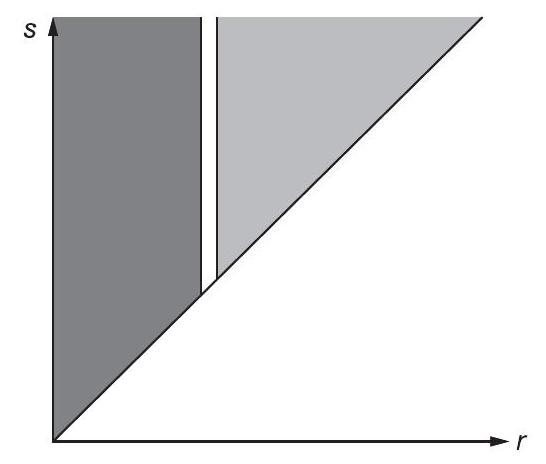
\includegraphics[max width=\textwidth, center]{2024_10_13_e0685a8ee0113ded3493g-71(1)}\\
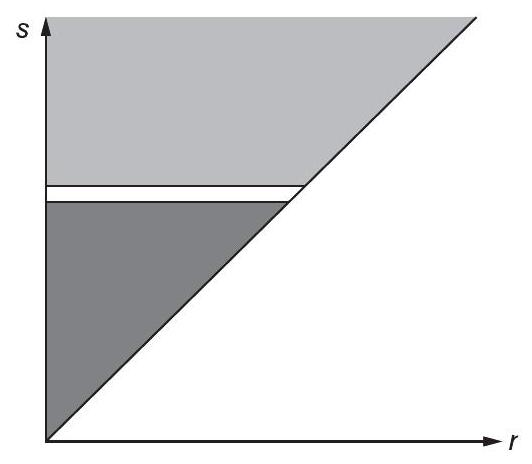
\includegraphics[max width=\textwidth, center]{2024_10_13_e0685a8ee0113ded3493g-71}

Figure 1.17 2-D integration region for Example 1.10.6. Left panel: inner integration over $s$; right panel: inner integration over $r$.\\
the form

$$
\int_{0}^{\infty} \frac{e^{-s}}{s} d s \int_{0}^{s} e^{-r} d r
$$

where the inner integral over $r$ is now elementary, evaluating to $1-e^{-s}$. This leaves us with a 1-D integral,

$$
\int_{0}^{\infty} \frac{e^{-s}}{s}\left(1-e^{-s}\right) d s
$$

Introducing a power series expansion for $1-e^{-s}$, this integral becomes

$$
\int_{0}^{\infty} \frac{e^{-s}}{s} \sum_{n=1}^{\infty} \frac{(-1)^{n-1} s^{n}}{n!}=\sum_{n=1}^{\infty} \frac{(-1)^{n-1}}{n!} \int_{0}^{\infty} s^{n-1} e^{-s} d s=\sum_{n=1}^{\infty} \frac{(-1)^{n-1}}{n!}(n-1)!
$$

where in the last step we have identified the $s$ integral (cf. Table 1.2) as $(n-1)$ !. We complete the evaluation by noting that $(n-1)!/ n!=1 / n$, so that the summation can be recognized as $\ln 2$, thereby giving the final result

$$
\int_{0}^{\infty} e^{-r} d r \int_{r}^{\infty} \frac{e^{-s}}{s} d s=\ln 2
$$

A significant change in the form of 2-D or 3-D integrals can sometimes be accomplished by changing between Cartesian and polar coordinate systems.

\section*{Example 1.10.7 EValuation in Polar COordinates}
In many calculus texts, the evaluation of $\int_{0}^{\infty} \exp \left(-x^{2}\right) d x$ is carried out by first converting it into a 2-D integral by taking its square, which is then written and evaluated in polar coordinates. Using the fact that $d x d y=r d r d \varphi$, we have

$$
\int_{0}^{\infty} d x e^{-x^{2}} \int_{0}^{\infty} d y e^{-y^{2}}=\int_{0}^{\pi / 2} d \varphi \int_{0}^{\infty} r d r e^{-r^{2}}=\frac{\pi}{2} \int_{0}^{\infty} \frac{1}{2} d u e^{-u}=\frac{\pi}{4}
$$

This yields the well-known result


\begin{equation*}
\int_{0}^{\infty} e^{-x^{2}} d x=\frac{1}{2} \sqrt{\pi} \tag{1.148}
\end{equation*}


\section*{Example 1.10.8 ATOMic Interaction InteGRAL}
For study of the interaction of a small atom with an electromagnetic field, one of the integrals that arises in a simple approximate treatment using Gaussian-type orbitals is (in dimensionless Cartesian coordinates)

$$
I=\int d \tau \frac{z^{2}}{\left(x^{2}+y^{2}+z^{2}\right)^{3 / 2}} e^{-\left(x^{2}+y^{2}+z^{2}\right)}
$$

where the range of the integration is the entire 3-D physical space $\left(\mathbb{R}^{3}\right)$. Of course, this is a problem better addressed in spherical polar coordinates $(r, \theta, \varphi)$, where $r$ is the distance from the origin of the coordinate system, $\theta$ is the polar angle (for the Earth, known as colatitude), and $\varphi$ is the azimuthal angle (longitude). The relevant conversion formulas are: $x^{2}+y^{2}+z^{2}=r^{2}$ and $z / r=\cos \theta$. The volume element is $d \tau=r^{2} \sin \theta d r d \theta d \varphi$, and the ranges of the new coordinates are $0 \leq r<\infty, 0 \leq \theta \leq \pi$, and $0 \leq \varphi<2 \pi$. In the spherical coordinates, our integral becomes

$$
\begin{aligned}
I & =\int d \tau \frac{\cos ^{2} \theta}{r} e^{-r^{2}}=\int_{0}^{\infty} d r r e^{-r^{2}} \int_{0}^{\pi} d \theta \cos ^{2} \theta \sin \theta \int_{0}^{2 \pi} d \varphi \\
& =\left(\frac{1}{2}\right)\left(\frac{2}{3}\right)(2 \pi)=\frac{2 \pi}{3}
\end{aligned}
$$

\section*{Remarks: Changes of Integration Variables}
In a 1-D integration, a change in the integration variable from, say, $x$ to $y=y(x)$ involves two adjustments: (1) the differential $d x$ must be replaced by $(d x / d y) d y$, and (2) the integration limits must be changed from $x_{1}, x_{2}$ to $y\left(x_{1}\right), y\left(x_{2}\right)$. If $y(x)$ is not single-valued\\
over the entire range $\left(x_{1}, x_{2}\right)$, the process becomes more complicated and we do not consider it further at this point.

For multiple integrals, the situation is considerably more complicated and demands some discussion. Illustrating for a double integral, initially in variables $x, y$, but transformed to an integration in variables $u, v$, the differential $d x d y$ must be transformed to $J d u d v$, where $J$, called the Jacobian of the transformation and sometimes symbolically represented as

$$
J=\frac{\partial(x, y)}{\partial(u, v)}
$$

may depend on the variables. For example, the conversion from 2-D Cartesian coordinates $x, y$ to plane polar coordinates $r, \theta$ involves the Jacobian

$$
J=\frac{\partial(x, y)}{\partial(r, \theta)}=r, \quad \text { so } \quad d x d y=r d r d \theta
$$

For some coordinate transformations the Jacobian is simple and of a well-known form, as in the foregoing example. We can confirm the value assigned to $J$ by noticing that the area (in $x y$ space) enclosed by boundaries at $r, r+d r, \theta$, and $\theta+d \theta$ is an infinitesimally distorted rectangle with two sides of length $d r$ and two of length $r d \theta$. See Fig. 1.18. For other transformations we may need general methods for obtaining Jacobians. Computation of Jacobians will be treated in detail in Section 4.4.

Of interest here is the determination of the transformed region of integration. In principle this issue is straightforward, but all too frequently one encounters situations (both in other texts and in research articles) where misleading and potentially incorrect arguments are presented. The confusion normally arises in cases for which at least a part of the boundary is at infinity. We illustrate with the conversion from 2-D Cartesian to plane polar coordinates. Figure 1.19 shows that if one integrates for $0 \leq \theta<2 \pi$ and $0 \leq r<a$, there are regions in the corners of a square (of side $2 a$ ) that are not included. If the integral is to be evaluated in the limit $a \rightarrow \infty$, it is both incorrect and meaningless to advance arguments about the "neglect" of contributions from these corner regions, as every point in these corners is ultimately included as $a$ is increased.

A similar, but slightly less obvious situation arises if we transform an integration over Cartesian coordinates $0 \leq x<\infty, 0 \leq y<\infty$, into one involving coordinates $u=x+y$,\\
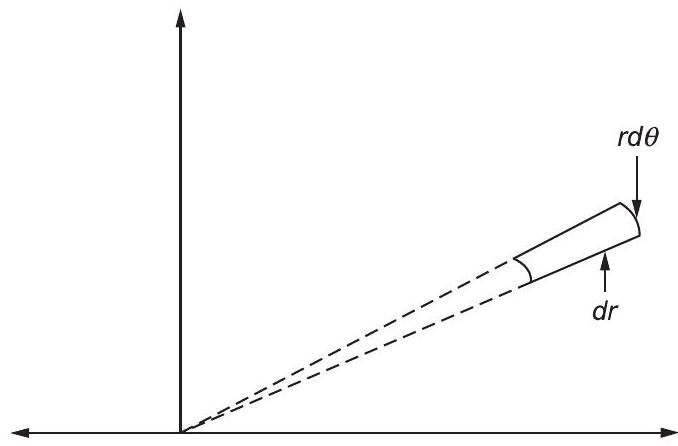
\includegraphics[max width=\textwidth, center]{2024_10_13_e0685a8ee0113ded3493g-73}

Figure 1.18 Element of area in plane polar coordinates.\\
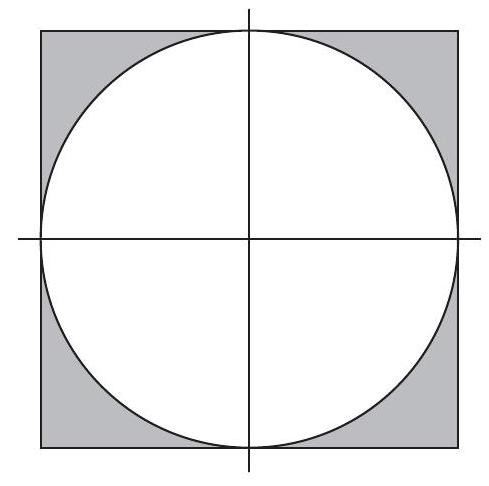
\includegraphics[max width=\textwidth, center]{2024_10_13_e0685a8ee0113ded3493g-74(1)}

FIGURE 1.19 2-D integration, Cartesian and plane polar coordinates.\\
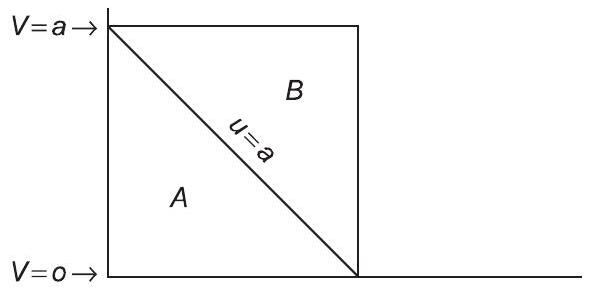
\includegraphics[max width=\textwidth, center]{2024_10_13_e0685a8ee0113ded3493g-74}

FIGURE 1.20 Integral in transformed coordinates.\\
$v=y$, with integration limits $0 \leq u<\infty, 0 \leq v \leq u$. See Fig. 1.20. Again it is incorrect and meaningless to make arguments justifying the "neglect" of the outer triangle (labeled $B$ in the figure). The relevant observation here is that ultimately, as the value of $u$ is increased, any arbitrary point in the quarter-plane becomes included in the region being integrated.

\section*{Exercises}
1.10.1 Use a recursive method to show that, for all positive integers $n, \Gamma(n)=(n-1)$ !. Evaluate the integrals in Exercises 1.10.2 through 1.10.9.\\
1.10.2 $\int_{0}^{\infty} \frac{\sin x}{x} d x$.

Hint. Multiply integrand by $e^{-a x}$ and take the limit $a \rightarrow 0$.\\
1.10.3 $\int_{0}^{\infty} \frac{d x}{\cosh x}$.

Hint. Expand the denominator is a way that converges for all relevant $x$.\\
1.10.4 $\int_{0}^{\infty} \frac{d x}{e^{a x}+1}$, for $a>0$.\\
1.10.5 $\int_{\pi}^{\infty} \frac{\sin x}{x^{2}} d x$\\
1.10.6 $\int_{0}^{\infty} \frac{e^{-x} \sin x}{x} d x$.\\
1.10.7 $\int_{0}^{x} \operatorname{erf}(t) d t$

The result can be expressed in terms of special functions in Table 1.2.\\
1.10.8 $\int_{1}^{x} E_{1}(t) d t$

Obtain a result in which the only special function is $E_{1}$.\\
1.10.9 $\int_{0}^{\infty} \frac{e^{-x}}{x+1} d x$\\
1.10.10 Show that $\int_{0}^{\infty}\left(\frac{\tan ^{-1} x}{x}\right)^{2} d x=\pi \ln 2$.

Hint. Integrate by parts, to linearize in $\tan ^{-1}$. Then replace $\tan ^{-1} x$ by $\tan ^{-1} a x$ and evaluate for $a=1$.\\
1.10.11 By direct integration in Cartesian coordinates, find the area of the ellipse defined by

$$
\frac{x^{2}}{a^{2}}+\frac{y^{2}}{b^{2}}=1
$$

1.10.12 A unit circle is divided into two pieces by a straight line whose distance of closest approach to the center is $1 / 2$ unit. By evaluating a suitable integral, find the area of the smaller piece thereby produced. Then use simple geometric considerations to verify your answer.

\subsection*{1.11 DIRAC DELTA FUNCTION}
Frequently we are faced with the problem of describing a quantity that is zero everywhere except at a single point, while at that point it is infinite in such a way that its integral over\\
any interval containing that point has a finite value. For this purpose it is useful to introduce the Dirac delta function, which is defined to have the properties


\begin{align*}
& \delta(x)=0, \quad x \neq 0  \tag{1.149}\\
& f(0)=\int_{a}^{b} f(x) \delta(x) d x \tag{1.150}
\end{align*}


where $f(x)$ is any well-behaved function and the integration includes the origin. As a special case of Eq. (1.150),


\begin{equation*}
\int_{-\infty}^{\infty} \delta(x) d x=1 \tag{1.151}
\end{equation*}


From Eq. (1.150), $\delta(x)$ must be an infinitely high, thin spike at $x=0$, as in the description of an impulsive force or the charge density for a point charge. The problem is that no such function exists, in the usual sense of function. However, the crucial property in Eq. (1.150) can be developed rigorously as the limit of a sequence of functions, a distribution. For example, the delta function may be approximated by any of the sequences of functions, Eqs. (1.152) to (1.155) and Figs. 1.21 and 1.22:


\begin{align*}
& \delta_{n}(x)= \begin{cases}0, & x<-\frac{1}{2 n} \\
n, & -\frac{1}{2 n}<x<\frac{1}{2 n} \\
0, & x>\frac{1}{2 n}\end{cases}  \tag{1.152}\\
& \delta_{n}(x)=\frac{n}{\sqrt{\pi}} \exp \left(-n^{2} x^{2}\right) \tag{1.153}
\end{align*}


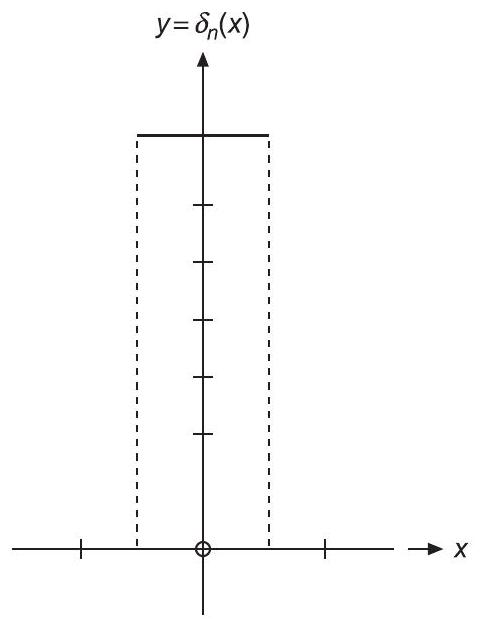
\includegraphics[max width=\textwidth, center]{2024_10_13_e0685a8ee0113ded3493g-76(1)}\\
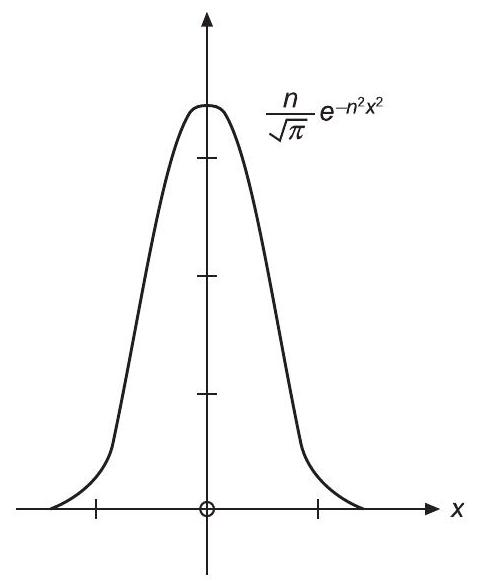
\includegraphics[max width=\textwidth, center]{2024_10_13_e0685a8ee0113ded3493g-76}

Figure $1.21 \delta$-Sequence function: left, Eq. (1.152); right, Eq. (1.153).\\
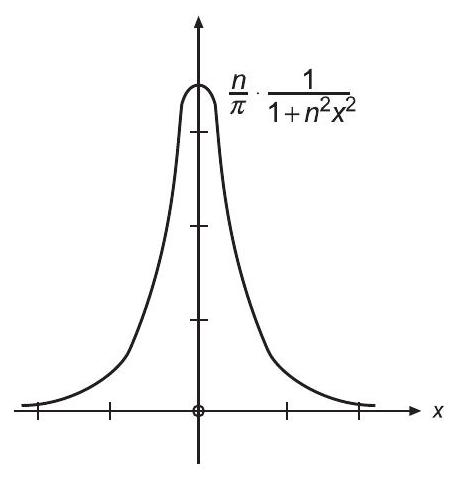
\includegraphics[max width=\textwidth, center]{2024_10_13_e0685a8ee0113ded3493g-77}\\
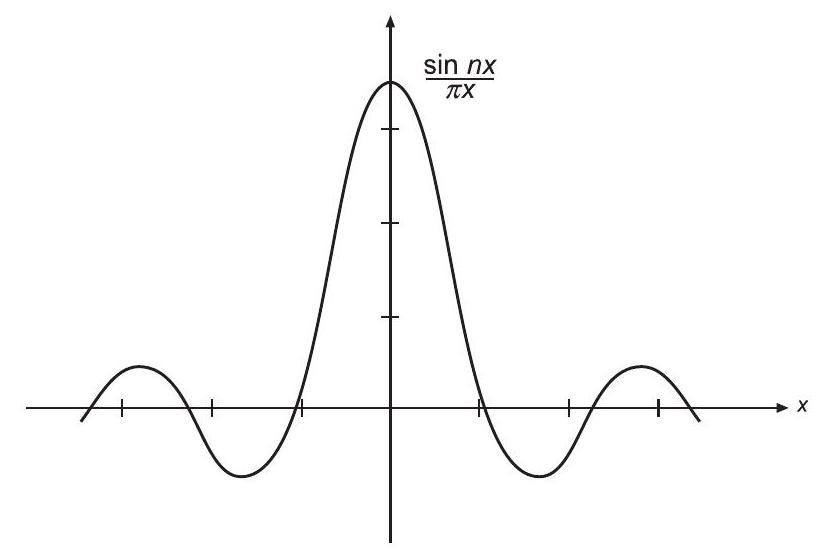
\includegraphics[max width=\textwidth, center]{2024_10_13_e0685a8ee0113ded3493g-77(1)}

FIGURE $1.22 \delta$-Sequence function: left, Eq. (1.154); right, Eq. (1.155).


\begin{align*}
& \delta_{n}(x)=\frac{n}{\pi} \frac{1}{1+n^{2} x^{2}}  \tag{1.154}\\
& \delta_{n}(x)=\frac{\sin n x}{\pi x}=\frac{1}{2 \pi} \int_{-n}^{n} e^{i x t} d t \tag{1.155}
\end{align*}


While all these sequences (and others) cause $\delta(x)$ to have the same properties, they differ somewhat in ease of use for various purposes. Equation (1.152) is useful in providing a simple derivation of the integral property, Eq. (1.150). Equation (1.153) is convenient to differentiate. Its derivatives lead to the Hermite polynomials. Equation (1.155) is particularly useful in Fourier analysis and in applications to quantum mechanics. In the theory of Fourier series, Eq. (1.155) often appears (modified) as the Dirichlet kernel:


\begin{equation*}
\delta_{n}(x)=\frac{1}{2 \pi} \frac{\sin \left[\left(n+\frac{1}{2}\right) x\right]}{\sin \left(\frac{1}{2} x\right)} \tag{1.156}
\end{equation*}


In using these approximations in Eq. (1.150) and elsewhere, we assume that $f(x)$ is well behaved-that it offers no problems at large $x$.

The forms for $\delta_{n}(x)$ given in Eqs. (1.152) to (1.155) all obviously peak strongly for large $n$ at $x=0$. They must also be scaled in agreement with Eq. (1.151). For the forms in Eqs. (1.152) and (1.154), verification of the scale is the topic of Exercises 1.11 .1 and 1.11.2. To check the scales of Eqs. (1.153) and (1.155), we need values of the integrals

$$
\int_{-\infty}^{\infty} e^{-n^{2} x^{2}} d x=\sqrt{\frac{\pi}{n}} \text { and } \int_{-\infty}^{\infty} \frac{\sin n x}{x} d x=\pi
$$

These results are respectively trivial extensions of Eqs. (1.148) and (11.107) (the latter of which we derive later).

For most physical purposes the forms describing delta functions are quite adequate. However, from a mathematical point of view the situation is still unsatisfactory. The limits

$$
\lim _{n \rightarrow \infty} \delta_{n}(x)
$$

\section*{do not exist.}
A way out of this difficulty is provided by the theory of distributions. Recognizing that Eq. (1.150) is the fundamental property, we focus our attention on it rather than on $\delta(x)$ itself. Equations (1.152) to (1.155) with $n=1,2,3 \ldots$ may be interpreted as sequences of normalized functions, and we may consistently write


\begin{equation*}
\int_{-\infty}^{\infty} \delta(x) f(x) d x \equiv \lim _{n \rightarrow \infty} \int \delta_{n}(x) f(x) d x \tag{1.157}
\end{equation*}


Thus, $\delta(x)$ is labeled a distribution (not a function) and is regarded as defined by Eq. (1.157). We might emphasize that the integral on the left-hand side of Eq. (1.157) is not a Riemann integral. ${ }^{8}$

\section*{Properties of $\delta(x)$}
\begin{itemize}
  \item From any of Eqs. (1.152) through (1.155) we see that Dirac's delta function must be even in $x, \delta(-x)=\delta(x)$.
  \item If $a>0$
\end{itemize}


\begin{equation*}
\delta(a x)=\frac{1}{a} \delta(x), \quad a>0 \tag{1.158}
\end{equation*}


Equation (1.158) can be proved by making the substitution $x=y / a$ :

$$
\int_{-\infty}^{\infty} f(x) \delta(a x) d x=\frac{1}{a} \int_{-\infty}^{\infty} f(y / a) \delta(y) d y=\frac{1}{a} f(0)
$$

If $a<0$, Eq. (1.158) becomes $\delta(a x)=\delta(x) /|a|$.

\begin{itemize}
  \item Shift of origin:
\end{itemize}


\begin{equation*}
\int_{-\infty}^{\infty} \delta\left(x-x_{0}\right) f(x) d x=f\left(x_{0}\right) \tag{1.159}
\end{equation*}


which can be proved by making the substitution $y=x-x_{0}$ and noting that when $y=0$, $x=x_{0}$.

\footnotetext{${ }^{8}$ It can be treated as a Stieltjes integral if desired; $\delta(x) d x$ is replaced by $d u(x)$, where $u(x)$ is the Heaviside step function (compare Exercise 1.11.9).
}\begin{itemize}
  \item If the argument of $\delta(x)$ is a function $g(x)$ with simple zeros at points $a_{i}$ on the real axis (and therefore $g^{\prime}\left(a_{i}\right) \neq 0$ ),
\end{itemize}


\begin{equation*}
\delta(g(x))=\sum_{i} \frac{\delta\left(x-a_{i}\right)}{\left|g^{\prime}\left(a_{i}\right)\right|} \tag{1.160}
\end{equation*}


To prove Eq. (1.160), we write

$$
\int_{-\infty}^{\infty} f(x) \delta(x) d x=\sum_{i} \int_{a_{i}-\varepsilon}^{a_{i}+\varepsilon} f(x) \delta\left(\left(x-a_{i}\right) g^{\prime}\left(a_{i}\right)\right) d x
$$

where we have decomposed the original integral into a sum of integrals over small intervals containing the zeros of $g(x)$. In these intervals, we replaced $g(x)$ by the leading term in its Taylor series. Applying Eqs. (1.158) and (1.159) to each term of the sum, we confirm Eq. (1.160).

\begin{itemize}
  \item Derivative of delta function:
\end{itemize}


\begin{equation*}
\int_{-\infty}^{\infty} f(x) \delta^{\prime}\left(x-x_{0}\right) d x=-\int_{-\infty}^{\infty} f^{\prime}(x) \delta\left(x-x_{0}\right) d x=-f^{\prime}\left(x_{0}\right) \tag{1.161}
\end{equation*}


Equation (1.161) can be taken as defining the derivative $\delta^{\prime}(x)$; it is evaluated by performing an integration by parts on any of the sequences defining the delta function.

\begin{itemize}
  \item In three dimensions, the delta function $\delta(\mathbf{r})$ is interpreted as $\delta(x) \delta(y) \delta(z)$, so it describes a function localized at the origin and with unit integrated weight, irrespective of the coordinate system in use. Thus, in spherical polar coordinates,
\end{itemize}


\begin{equation*}
\iiint f\left(\mathbf{r}_{2}\right) \delta\left(\mathbf{r}_{2}-\mathbf{r}_{1}\right) r_{2}^{2} d r_{2} \sin \theta_{2} d \theta_{2} d \phi_{2}=f\left(\mathbf{r}_{1}\right) \tag{1.162}
\end{equation*}


\begin{itemize}
  \item Equation (1.155) corresponds in the limit to
\end{itemize}


\begin{equation*}
\delta(t-x)=\frac{1}{2 \pi} \int_{-\infty}^{\infty} \exp (i \omega(t-x)) d \omega \tag{1.163}
\end{equation*}


with the understanding that this has meaning only when under an integral sign. In that context it is extremely useful for the simplification of Fourier integrals (Chapter 20).

\begin{itemize}
  \item Expansions of $\delta(x)$ are addressed in Chapter 5. See Example 5.1.7.
\end{itemize}

\section*{Kronecker Delta}
It is sometimes useful to have a symbol that is the discrete analog of the Dirac delta function, with the property that it is unity when the discrete variable has a certain value, and zero otherwise. A quantity with these properties is known as the Kronecker delta, defined for indices $i$ and $j$ as

\[
\delta_{i j}= \begin{cases}1, & i=j  \tag{1.164}\\ 0, & i \neq j\end{cases}
\]

Frequent uses of this symbol are to select a special term from a summation, or to have one functional form for all nonzero values of an index, but a different form when the index is zero. Examples:

$$
\sum_{i j} f_{i j} \delta_{i j}=\sum_{i} f_{i i}, \quad C_{n}=\frac{1}{1+\delta_{n 0}} \frac{2 \pi}{L}
$$

\section*{Exercises}
\subsection*{1.11.1 Let}
$$
\delta_{n}(x)= \begin{cases}0, & x<-\frac{1}{2 n} \\ n, & -\frac{1}{2 n}<x<\frac{1}{2 n} \\ 0, & \frac{1}{2 n}<x\end{cases}
$$

Show that

$$
\lim _{n \rightarrow \infty} \int_{-\infty}^{\infty} f(x) \delta_{n}(x) d x=f(0)
$$

assuming that $f(x)$ is continuous at $x=0$.\\
1.11.2 For

$$
\delta_{n}(x)=\frac{n}{\pi} \frac{1}{1+n^{2} x^{2}}
$$

show that

$$
\int_{-\infty}^{\infty} \delta_{n}(x) d x=1
$$

1.11.3 Fejer's method of summing series is associated with the function

$$
\delta_{n}(t)=\frac{1}{2 \pi n}\left[\frac{\sin (n t / 2)}{\sin (t / 2)}\right]^{2}
$$

Show that $\delta_{n}(t)$ is a delta distribution, in the sense that

$$
\lim _{n \rightarrow \infty} \frac{1}{2 \pi n} \int_{-\infty}^{\infty} f(t)\left[\frac{\sin (n t / 2)}{\sin (t / 2)}\right]^{2} d t=f(0)
$$

1.11.4 Prove that

$$
\delta\left[a\left(x-x_{1}\right)\right]=\frac{1}{a} \delta\left(x-x_{1}\right)
$$

Note. If $\delta\left[a\left(x-x_{1}\right)\right]$ is considered even, relative to $x_{1}$, the relation holds for negative $a$ and $1 / a$ may be replaced by $1 /|a|$.\\
1.11.5 Show that

$$
\delta\left[\left(x-x_{1}\right)\left(x-x_{2}\right)\right]=\left[\delta\left(x-x_{1}\right)+\delta\left(x-x_{2}\right)\right] /\left|x_{1}-x_{2}\right|
$$

Hint. Try using Exercise 1.11.4.\\
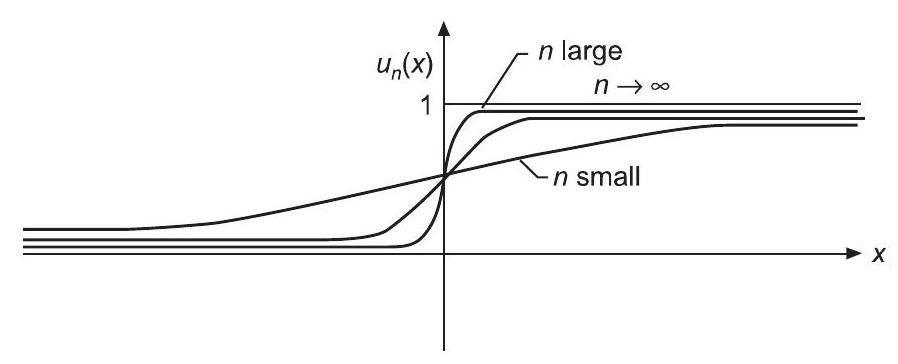
\includegraphics[max width=\textwidth, center]{2024_10_13_e0685a8ee0113ded3493g-81}

Figure 1.23 Heaviside unit step function.\\
1.11.6 Using the Gauss error curve delta sequence $\delta_{n}=\frac{n}{\sqrt{\pi}} e^{-n^{2} x^{2}}$, show that

$$
x \frac{d}{d x} \delta(x)=-\delta(x)
$$

treating $\delta(x)$ and its derivative as in Eq. (1.157).\\
1.11.7 Show that

$$
\int_{-\infty}^{\infty} \delta^{\prime}(x) f(x) d x=-f^{\prime}(0)
$$

Here we assume that $f^{\prime}(x)$ is continuous at $x=0$.\\
1.11.8 Prove that

$$
\delta(f(x))=\left|\frac{d f(x)}{d x}\right|_{x=x_{0}}^{-1} \delta\left(x-x_{0}\right)
$$

where $x_{0}$ is chosen so that $f\left(x_{0}\right)=0$.\\
Hint. Note that $\delta(f) d f=\delta(x) d x$.\\
1.11.9 (a) If we define a sequence $\delta_{n}(x)=n /\left(2 \cosh ^{2} n x\right)$, show that

$$
\int_{-\infty}^{\infty} \delta_{n}(x) d x=1, \quad \text { independent of } n
$$

(b) Continuing this analysis, show that ${ }^{9}$

$$
\int_{-\infty}^{x} \delta_{n}(x) d x=\frac{1}{2}[1+\tanh n x] \equiv u_{n}(x)
$$

and

$$
\lim _{n \rightarrow \infty} u_{n}(x)= \begin{cases}0, & x<0 \\ 1, & x>0\end{cases}
$$

This is the Heaviside unit step function (Fig. 1.23).

\footnotetext{${ }^{9}$ Many other symbols are used for this function. This is the AMS-55 notation (in Additional Readings, see Abramowitz and Stegun): $u$ for unit.
}
\end{document}